\documentclass[10pt]{article}
\usepackage[a4paper,top=2cm,bottom=2cm,left=2cm,right=2cm,marginparwidth=2cm]{geometry}
\linespread{1.5}
\usepackage[utf8]{inputenc}
\usepackage{multirow}
\usepackage{graphicx}
\usepackage{listings}
\usepackage{xcolor}
\usepackage[colorlinks=true, allcolors=blue]{hyperref}
\usepackage{amsmath,amsthm,amssymb,amsfonts}
\usepackage{float}
\usepackage{listings}
\usepackage{subfigure}
\usepackage{tikz}
\usepackage{tocloft}
\renewcommand{\cftsecleader}{\textcolor{red}{\cftdotfill{\cftsecdotsep}}} % context color
% \lstset{ %
%   language=R,                % the language of the code
%   basicstyle=\footnotesize,           % the size of the fonts that are used for the code
%   numbers=left,                   % where to put the line-numbers
%   numberstyle=\tiny\color[rgb]{0.4,0.2,0.2},  % the style that is used for the line-numbers
%   stepnumber=2,                   % the step between two line-numbers. If it's 1, each line 
%                                   % will be numbered
%   numbersep=12pt,                  % how far the line-numbers are from the code
%   backgroundcolor=\color{white},      % choose the background color. You must add \RequirePackage{color}
%   showspaces=false,               % show spaces adding particular underscores
%   showstringspaces=false,         % underline spaces within strings
%   showtabs=false,                 % show tabs within strings adding particular underscores
%   %frame=single,                   % adds a frame around the code
%   rulecolor=\color{black},        % if not set, the frame-color may be changed on line-breaks within not-black text (e.g. commens (green here))
%   tabsize=2,                      % sets default tabsize to 2 spaces
%   captionpos=b,                   % sets the caption-position to bottom
%   breaklines=true,                % sets automatic line breaking
%   breakatwhitespace=false,        % sets if automatic breaks should only happen at whitespace
%   title=\lstname,                   % show the filename of files included with \lstinputlisting;
%                                   % also try caption instead of title
%   keywordstyle=\color[rgb]{0.9,0.5,0.5},          % keyword style
%   commentstyle=\color[rgb]{0.4,0.3,0.9},       % comment style
%   stringstyle=\color[rgb]{0.35,0.85,0.5},         % string literal style
%   escapeinside={\%*}{*)},            % if you want to add LaTeX within your code
%   morekeywords={*,...}               % if you want to add more keywords to the set
% }

\definecolor{codegreen}{rgb}{0,0.6,0}
\definecolor{codegray}{rgb}{0.5,0.5,0.5}
\definecolor{codepurple}{rgb}{0.58,0,0.82}
\definecolor{backcolour}{rgb}{0.95,0.95,0.92}

\lstdefinestyle{mystyle}{
    backgroundcolor=\color{backcolour},   
    commentstyle=\color{codegreen},
    keywordstyle=\color{magenta},
    numberstyle=\tiny\color{codegray},
    stringstyle=\color{codepurple},
    basicstyle=\ttfamily\footnotesize,
    breakatwhitespace=false,         
    breaklines=true,                 
    captionpos=b,                    
    keepspaces=true,                 
    numbers=left,                    
    numbersep=5pt,                  
    showspaces=false,                
    showstringspaces=false,
    showtabs=false,                  
    tabsize=2
}

\lstset{style=mystyle}
\usepackage{blindtext}
\usepackage{titlesec}
\usepackage{longtable}
\graphicspath{ {./images/} }
\renewcommand{\arraystretch}{0.8}
\usepackage{amsmath} % Allows you to do equations
\usepackage{fancyhdr} % Formats the header
\setlength{\parindent}{0pt} % no paragraph indents
\setlength{\parskip}{1em} % paragraphs separated by one line
\usepackage[style=authoryear-ibid,backend=biber,maxbibnames=99,maxcitenames=2,uniquelist=false,isbn=false,url=true,hyperref=true,eprint=false,doi=true,giveninits=true,uniquename=init]{biblatex} % Allows you to do citations - does Harvard style and compatible with Zotero
%\usepackage[style=authoryear, citestyle=authoryear, backend=biber]{biblatex}
\usepackage[colorlinks,citecolor=blue,urlcolor=blue,bookmarks=false,hypertexnames=true]{hyperref} 

\defbibenvironment{bibliography}
  {\list
     {\printtext[labelalphawidth]{%
        \printfield{labelprefix}%
        \printfield{labelalpha}%
        \printfield{extraalpha}}}
     {\setlength{\labelwidth}{\labelalphawidth}%
      \setlength{\leftmargin}{\labelwidth}%
      \setlength{\labelsep}{\biblabelsep}%
      \addtolength{\leftmargin}{\labelsep}%
      \setlength{\itemsep}{\bibitemsep}%
      \setlength{\parsep}{\bibparsep}}%
      \renewcommand*{\makelabel}[1]{##1\hss}}
  {\endlist}
  {\item}
\addbibresource{name.bib}

\renewcommand{\headrulewidth}{0pt}
\geometry{letterpaper, portrait, margin=1in}
\setlength{\headheight}{14.49998pt}

\newcommand\titleofdoc{ECON 723: Econometrics 2} %%%%% Put your document title in this argument
\newcommand\GroupName{Kim Jin, Christian Newey, Amber Kou, Zhonghu Wang, Yu Chen} %%%%% Put your group name here. If you are the only member of the group, just put your name

\begin{document}
\addtocontents{toc}{\protect\hypersetup{linkcolor=red}}

\begin{titlepage}
   \begin{center}
        \vspace*{3cm} % Adjust spacings to ensure the title page is generally filled with text

        \Large{\titleofdoc} 

        \vspace{0.5cm}
        \LARGE{Group Project 1}
            
        \vspace{2 cm}
        \Large{}
            
        \vspace{2 cm}
        \Large{\GroupName}
       
        \vspace{0.25cm}
        \large{}
       
        \vspace{1 cm}
        \Large{23 Aug 2023}
        
        \vspace{0.25 cm}
        \Large{University of Auckland}
       

       \vfill
    \end{center}
\end{titlepage}

\newpage

\setcounter{page}{1}
\pagestyle{fancy}
\fancyhf{}
\rhead{\thepage}
\lhead{\GroupName; \titleofdoc}







\section*{Abstract}
Our report utilises New Zealand and United States data to examine the impact of returns across the nations on the exchange rate between them, working to see if we could identify the presence of UIP. In addition the effect of yield curve slopes are considered given their possibility of reflecting outside factors on the exchange rate. The work is based on the paper “Exchange-Rate Risk and Business Cycles” from 2019 by Lloyd and Marin \footnote{\cite{lloyd2020exchange}\label{lloyd2020exchange}} and works to examine the same areas that are discussed in section 2, except focussed on this specific exchange rate relation of the United States and New Zealand.

The comprehensive resources requisite for recreating this paper, including the datasets and codes are accessible at the designated GitHub repository: \url{https://github.com/Kim-Jin-1998/ECON-723-group-project-1}

\newpage

\section*{Table}

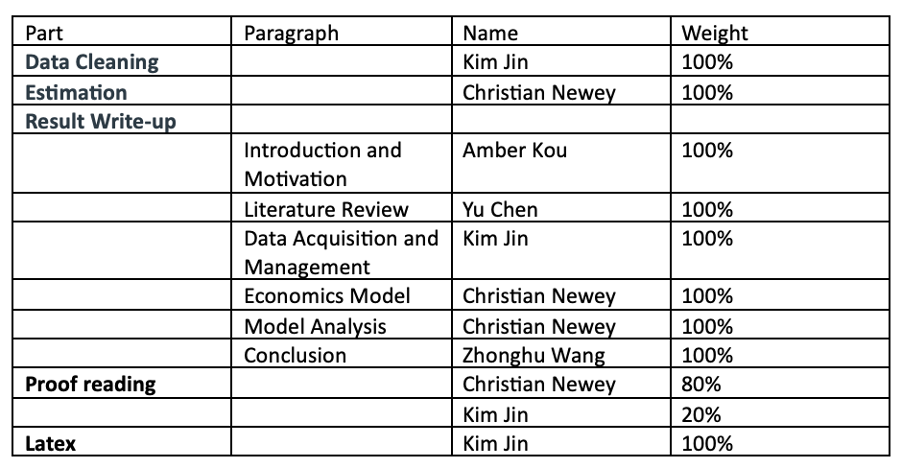
\includegraphics[scale =1]{picture/table.png}


\newpage
\tableofcontents

\newpage
\pagenumbering{arabic}

\section{Introduction}
The standard principle of uncovered interest parity (UIP) states that the interest rate differential between two countries should equal to the expected fluctuation in their exchange rates over the same period. Essentially, a country with a higher interest rate, according to UIP, should anticipate a corresponding depreciation in its currency. However, empirical evidence and prior literature often contradict this prediction, revealing that currencies with higher interest rates tend to appreciate rather than depreciate \footnote{\cite{kalemli2021five}\label{kalemli2021five}}. This inconsistency introduces the UIP puzzle.

\subsection{Motivation}
As a vast topic itself, UIP has been investigated from various perspectives. Firstly, The Uncovered Interest Parity (UIP) plays a pivotal role in shaping the monetary and interest rate policies of nations. Governments, especially those of emerging economies, often grapple with the challenge of ensuring stability in their financial markets. The UIP condition, which equates returns to different currencies, serves as a guiding principle for policymakers. As highlighted by \cite{ozigbu2018interest}, the monetary policy rate can significantly influence the performance of vital sectors, such as the industrial sector. Specifically, in the long run, this rate can pose substantial constraints to the effective functioning of these sectors. Thus, understanding and researching UIP becomes paramount for governments aiming to strike a balance in their monetary policies.

Secondly, whether for retail or institutional investors, the UIP condition holds significant implications. At the heart of investment decisions lies the interplay of risk and return. UIP, with its emphasis on currency returns, directly impacts investor sentiments. \cite{ur2013investor} underscores the profound influence of investor sentiments on exchange rate volatility. This sentiment-driven volatility, in turn, can lead to deviations from the UIP condition, resulting in potential risk premiums or even unexpected investment losses. Thus, being unfamiliar with UIP can predispose investors to emotional reactions, potentially resulting in avoidable investment losses. On the contrary, a deep understanding of UIP provides investors with the insight needed to navigate the complexities of international finance adeptly.

Thirdly, on the global stage, the UIP condition manifests differently across advanced economies (AEs) and emerging markets (EMs), and prior empirical research has confirmed that. While AEs often witness fluctuations in currency returns, EMs predominantly experience positive excess currency returns \footnote{As above \hyperref[kalemli2021five]{n2}}. Such disparities underscore the importance of UIP in international economics. The deviations from UIP in emerging markets, for instance, are often driven by factors such as policy uncertainty, which can be distinct from those in advanced economies\footnote{As above \hyperref[kalemli2021five]{n2}}. Therefore, researching UIP is not just an academic endeavour but a necessity for understanding the intricacies of global economic dynamics.

Fourth, Asset pricing at its core, revolves around determining the appropriate value of assets, factoring in various risks. One such risk, especially pertinent in the realm of international finance, is the exchange rate risk premium. UIP, with its focus on equating returns to different currencies, is intrinsically linked to this risk premium. The deviations from UIP, often resulting from policy uncertainties or global risk sentiments, directly influence the risk premiums associated with currencies\footnote{As above \hyperref[kalemli2021five]{n2}}. Moreover, \cite{joseph2021pricing} concluded that investors view risk premium as an important factor affecting portfolio returns. Thus, from an asset pricing standpoint, delving deep into UIP is crucial for accurate valuation and risk assessment.

\subsection{Data processing and result interpretation}
Our data exhibits non-stationarity and lacks a clear trend therefore it will not be perfectly suitable for general timer series models such as AR, ARMA, and ARIMA and sole reliance on simple linear regression might result in omitted variable bias, necessitating more robust methods. Consequently, we employed the Random Forest Model in machine learning to predict missing yield rates using swap and interbank rates, forming the final dataset. Then we executed three regression models to assess the UIP theory between New Zealand and Australia. The initial regression suggests that UIP is more applicable at longer horizons and less so at shorter ones. The subsequent regression concluded the slope variable's insignificance concerning the exchange rate between New Zealand and the U.S. The final stage regression reveals that the adjusted R-squared amplifies with elongated prediction horizons, further emphasizing UIP's restricted relevance at reduced horizons. Moreover, incorporating the slope variable in regressions augments the model's accuracy, indicating the yield curves' relative slope as a crucial element of the exchange rate risk premium.

\section{Literature Review}
Many articles have shown that the yield curve factor has a significant relationship with exchange-rate risk premia. In other words, the yield curve can be used to predict exchange-rate risk premia.Based on the zero-coupon yield data and the UIP method, \cite{chen2013does} tried to use the Nelson-Siegel factor in the relative yield curves of the two countries to predict future exchange rate changes. That is, they try to predict future exchange rate movements among countries through the long-term and short-term cross-border yield curve differences of the three countries. The final research results show that the relative yield curves of the three countries can only predict the short-term exchange rate changes of the two parties in the future for about 1 month to 2 years. However, according to this result, the paper did not draw the conclusion that long-term exchange rate movements can be predicted by differences in yield curves among countries. And \cite{grab2018predicting} also only concluded that they can use a linear combination of bond yield curves which is highly negatively correlated with the curvature factor in the Nelson Siegel model to predict the future one to six months Short-term interest rate and exchange rate risk premiums. 

Yield curve is considered as a tool to predict the business cycle risk. \cite{hasse2022does} using dynamic panels and 45-year datasets from 13 countries to examine the relationship between yield curve and business cycle across countries. The results show that there is indeed a significant relationship between yield and economic activity. In other words, economic activity can be observed through the yield curve, that is,a steeper yield curve predicts good economic conditions, and good economic conditions lead to higher interest rates. \cite{riddiough2018business} uses the exchange rate habitual model to link the business cycle with the forecasted excess return on currency, in other words, the business cycle is related to the forecasted exchange rate. Specifically, when the economy is in recession, domestic interest rates are generally lower and compared with foreign countries, there are many risk-averse people in the country, so they will demand a premium to hold foreign exchange to obtain a positive excess return.

\cite{kaminska2013global} study the relationship between the term structure of international interest rates and exchange rates in three countries with  a no-arbitrage affine term structure model. Besides, \cite{ang2010yield} also showing that under the no-arbitrage term structure, the price difference of the conditional volatility of the stochastic discount factor of each country determines the expected return of the exchange rate, that is, the conditional volatility of the stochastic discount factor of each country and the return rate curves are significantly related as long as any factor about the term structure of yields is used to predict the foreign exchange risk premium. Therefore, in our paper, we also examine the significant relationship between the yield curve and ERRP under the no-arbitrage term structure.






\section{Data Acquisition and Management}

\subsection{Data Sources}
Our dataset comprises the monthly yields for 1, 2, 5, and 10-year periods for both New Zealand (NZ) and the United States (US). Additionally, it includes the exchange rates and 90 day bank bill yields from both countries.



\subsection{Data Enrichment}

Being a time series dataset, our primary focus is to ascertain the presence of trends, seasonality, autocorrelation, and its stationarity. For this, we decomposed the time series data into its constituent elements: the seasonal, trend, and random (or irregular) components.

To achieve this, we utilized the decompose model. An analysis of the resultant table suggests an absence of a distinct trend. However, the data exhibits clear seasonality while appearing somewhat random.

\[Y_{t}=Trend_{t}+Seasonal_{t}+Random_{t}\]

From the table, we can see that there is not a clear trend and clearly the data is seasonal, and it looks random.


\tikzset{global scale/.style={
    scale=#1,
    every node/.append style={scale=#1}
  }
}
\begin{figure}[H]
    \centering
        \begin{tikzpicture}[global scale = 1]
            \node[anchor=south west,inner sep=0] at (0,0) {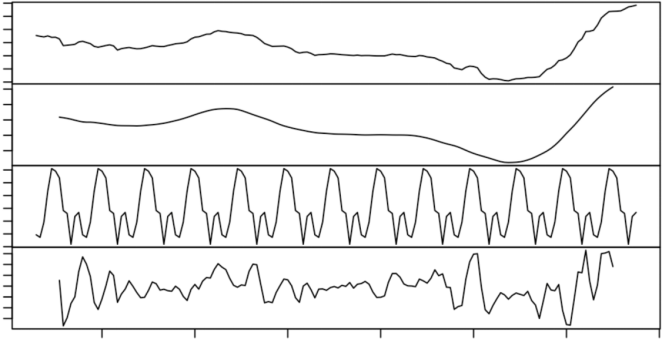
\includegraphics[width=0.8\textwidth]{picture/Decomposition.png}};
            \node at (2.1,-0.3){\small 2012};
            \node at (3.9,-0.3){\small 2014};
            \node at (5.7,-0.3){\small 2016};
            \node at (7.6,-0.3){\small 2018};
            \node at (9.5,-0.3){\small 2020};
            \node at (11.4,-0.3){\small 2022};
            \node at (13.2,-0.3){\small 2024};
            \node at (6.4,-1){\textbf{\footnotesize Time}};

            \node at(-0.2,0.35)[rotate=90]{\small -0.3}; 
            \node at(-0.2,1.25)[rotate=90]{\small 0.1}; 
            \node at(-0.2,1.8)[rotate=90]{\small -0.06}; 
            \node at(-0.2,2.9)[rotate=90]{\small 0.02}; 
            \node at(-0.2,3.75)[rotate=90]{\small 1}; 
            \node at(-0.2,4.35)[rotate=90]{\small 3}; 
            \node at(-0.2,4.95)[rotate=90]{\small 5};
             \node at(-0.2,5.1)[rotate=90]{\small 0};
             \node at(-0.2,5.62)[rotate=90]{\small 2};
              \node at(-0.2,6.15)[rotate=90]{\small 4};
               \node at(-0.2,6.75)[rotate=90]{\small 6};
               \node at(-1,3.5)[rotate=90]{ \textbf{\footnotesize random seasonal trend observed}};
        \end{tikzpicture}
    \caption{Decomposition of additive time series}
    \label{Decomposition1}
\end{figure}

% \begin{figure}[H]
%     \centering
%     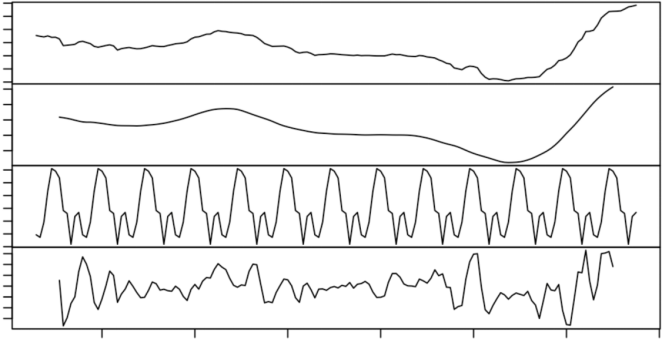
\includegraphics[width=0.8\textwidth]{picture/Decomposition.png}
%   \vspace{20pt}\caption{\hyperref[Decomposition1]{Decomposition of additive time series}}
%   %  \label{Decomposition1}
%     \begin{picture}(0,0)
%         \put(0.37\textwidth,0.097\textwidth){\makebox(0,0)[lt]{\small{{2024}}}}
%         \put(0.26\textwidth,0.097\textwidth){\makebox(0,0)[lt]{\small{{2022}}}}
%         \put(0.15\textwidth,0.097\textwidth){\makebox(0,0)[lt]{\small{{2020}}}}
%         \put(0.04\textwidth,0.097\textwidth){\makebox(0,0)[lt]{\small{{2018}}}}
%         \put(-0.07\textwidth,0.097\textwidth){\makebox(0,0)[lt]{\small{{2016}}}}
%         \put(-0.18\textwidth,0.097\textwidth){\makebox(0,0)[lt]{\small{{2014}}}}
%         \put(-0.29\textwidth,0.097\textwidth){\makebox(0,0)[lt]{\small{{2012}}}}

%         \put(-0.43\textwidth,0.14\textwidth){\makebox(0,0)[lt]{\rotatebox{90}{\small{-0.3}}}}
%         \put(-0.43\textwidth,0.19\textwidth){\makebox(0,0)[lt]{\rotatebox{90}{\small{0.1}}}}
%         \put(-0.43\textwidth,0.23\textwidth){\makebox(0,0)[lt]{\rotatebox{90}{\small{-0.06}}}}
%         \put(-0.43\textwidth,0.286\textwidth){\makebox(0,0)[lt]{\rotatebox{90}{\small{0.02}}}}
%         \put(-0.43\textwidth,0.334\textwidth){\makebox(0,0)[lt]{\rotatebox{90}{\small{1}}}}
%         \put(-0.43\textwidth,0.37\textwidth){\makebox(0,0)[lt]{\rotatebox{90}{\small{3}}}}
%         \put(-0.43\textwidth,0.415\textwidth){\makebox(0,0)[lt]{\rotatebox{90}{\small{50}}}}
%         \put(-0.43\textwidth,0.45\textwidth){\makebox(0,0)[lt]{\rotatebox{90}{\small{2}}}}
%         \put(-0.43\textwidth,0.48\textwidth){\makebox(0,0)[lt]{\rotatebox{90}{\small{4}}}}
%         \put(-0.43\textwidth,0.51\textwidth){\makebox(0,0)[lt]{\rotatebox{90}{\small{6}}}}

%         \put(-0.02\textwidth,0.07\textwidth){\makebox(0,0)[lt]{\textbf{Time}}}
%         \put(-0.47\textwidth,0.47\textwidth){\makebox(0,0)[lt]{\rotatebox{90}{\textbf{random seasonal trend observed}}}}

%     \end{picture}
% \end{figure}


It's worth noting that a non-stationary time series will always contain the a random, volatile component. This component encapsulates minor fluctuations around the overarching trend, cycle, and seasonal elements. While unpredictable, this can typically be modeled as random observations deriving from a certain distribution, often represented as \(N(0,\sigma^2)\).
\subsubsection{ACF test}

\tikzset{global scale/.style={
    scale=#1,
    every node/.append style={scale=#1}
  }
}
\begin{figure}[H]
    \centering
        \begin{tikzpicture}[global scale = 1]
            \node[anchor=south west,inner sep=0] at (0,0) {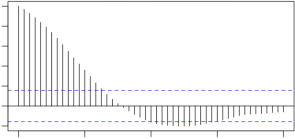
\includegraphics[width=0.3\textwidth]{picture/Series1.png}};
    \node at(0.35,-0.15){\small 0};
    \node at(1.42,-0.15){\small 1};     
    \node at(2.56,-0.15){\small 2};
    \node at(3.67,-0.15){\small 3};   
    \node at(4.78,-0.15){\small 4};
    \node at(2.5,-0.8){\small Lag};
    \node at(2.63,2.8){\textbf{Series swap.ts}};

    \node at(-0.2,0.2)[rotate=90]{\small -0.2};        
    \node at(-0.2,0.9)[rotate=90]{\small 0.2};  
    \node at(-0.2,1.6)[rotate=90]{\small 0.6};  
    \node at(-0.2,2.3)[rotate=90]{\small 1.0};  
    \node at(-1,1.2)[rotate=90]{\small ACF};        

    
            \node[anchor=south west,inner sep=0] at (7,0) {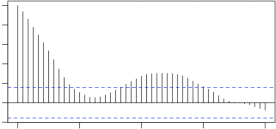
\includegraphics[width=0.3\textwidth]{picture/Series2.png}};
            \node at(9.5,2.8){\textbf{Series (swap.ts-mean(swap.ts))$^2$}};
     \node at(7+0.35,-0.15){\small 0};
    \node at(7+1.42,-0.15){\small 1};     
    \node at(7+2.56,-0.15){\small 2};
    \node at(7+3.67,-0.15){\small 3};   
    \node at(7+4.78,-0.15){\small 4};
    \node at(7+2.63,-0.8){\small Lag};

    \node at(7+-0.2,0.2)[rotate=90]{\small -0.2};        
    \node at(7+-0.2,0.9)[rotate=90]{\small 0.2};  
    \node at(7+-0.2,1.6)[rotate=90]{\small 0.6};  
    \node at(7+-0.2,2.3)[rotate=90]{\small 1.0};  
    \node at(7+-1,1.2)[rotate=90]{\small ACF};   
        \end{tikzpicture}
    \caption{}
    \label{Series1}
\end{figure}

The Autocorrelation Function (ACF) points to a robust autocorrelation at lag(16) in the swap rate, hinting at seasonality. It is observed that as time progresses, the positive correlation tends to wane until it turns negative. However, this correlation also diminishes with increasing lag. Our primary focus is on data points outside the blue region, given their high statistical significance. An analysis of heteroscedasticity corroborates these findings.

\begin{lstlisting}[language = R]
        Augmented Dickey-Fuller Test
    
data: swap.ts
Dickey-Fuller  =-1.0953, Lag order  =5, p -value  =0.9203  
alternative hypothesis: stationary    

\end{lstlisting}

\subsubsection{The ADF test:}

For a time series to be classified as stationary, it must be devoid of trends or seasonal impacts. If the procured p-value surpasses the significance level of 0.05 and the ADF statistic is greater than any of the established critical values, we have no compelling reason to reject the null hypothesis. As such, our conclusion is that the time series is non-stationary.

Furthermore, a similar analysis was conducted for the two-year period swap rate and the one-year period interbank rate. The findings paralleled the observations made previously.

\subsubsection{The test of 2 year period swap rates}

\begin{lstlisting}[language = R]
        Augmented Dickey-Fuller Test
        
data: swap.ts1
Dickey-Fuller  = -0.96763, Lag order  = 5, p-value  = 0.9405 
alternative hypothesis: stationary  

\end{lstlisting}


\begin{figure}[H]
    \centering
        \begin{tikzpicture}[global scale = 1]
            \node[anchor=south west,inner sep=0] at (0,0) {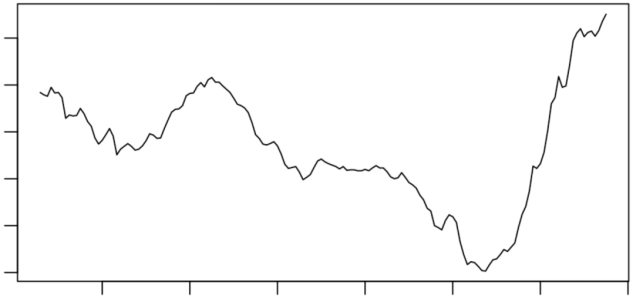
\includegraphics[width=0.8\textwidth]{picture/Swap.png}};
    \node at(12.95,-0.3){\small 2024};
    \node at(11.1,-0.3){\small 2022};     
    \node at(9.4,-0.3){\small 2020}; 
    \node at(7.5,-0.3){\small 2018}; 
    \node at(5.7,-0.3){\small 2016}; 
    \node at(3.9,-0.3){\small 2014}; 
    \node at(2.2,-0.3){\small 2012};    
    \node at(6.7,-1){\small month};   


    

    \node at(-0.3,0.5)[rotate=90]{\small 0};    
    \node at(-0.3,1.5)[rotate=90]{\small 1};   
    \node at(-0.3,2.45)[rotate=90]{\small 2};    
    \node at(-0.3,3.4)[rotate=90]{\small 3};   
    \node at(-0.3,4.4)[rotate=90]{\small 4};    
    \node at(-0.3,5.4)[rotate=90]{\small 5};   
    \node at(-1,3)[rotate=90]{\small Swap Rate in Percent};   
    
        \end{tikzpicture}
    \caption{Swap Rate for 2 Year Period}
\label{Swap}
\end{figure}


\begin{figure}[H]
    \centering
        \begin{tikzpicture}[global scale = 1]
            \node[anchor=south west,inner sep=0] at (0,0) {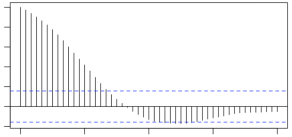
\includegraphics[width=0.3\textwidth]{picture/Series2_1.png}};
    \node at(0.35,-0.15){\small 0};
    \node at(1.46,-0.15){\small 1};     
    \node at(2.55,-0.15){\small 2};
    \node at(3.65,-0.15){\small 3};   
    \node at(4.75,-0.15){\small 4};
    \node at(2.5,-0.8){\small Lag};
    \node at(2.63,2.8){\textbf{Series swap.ts1}};

    \node at(-0.2,0.2)[rotate=90]{\small -0.2};        
    \node at(-0.2,0.9)[rotate=90]{\small 0.2};  
    \node at(-0.2,1.6)[rotate=90]{\small 0.6};  
    \node at(-0.2,2.3)[rotate=90]{\small 1.0};  
    \node at(-1,1.2)[rotate=90]{\small ACF};        

    
            \node[anchor=south west,inner sep=0] at (7,0) {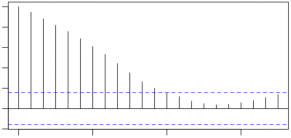
\includegraphics[width=0.3\textwidth]{picture/Series2_2.png}};
            \node at(9.5,2.8){\textbf{Series (swap.ts1-mean(swap.ts1))$^2$}};

    \node at(7+0.4,-0.15){\small 0.0};     
    \node at(7+1.6,-0.15){\small 0.5};
    \node at(7+2.8,-0.15){\small 1.0};   
    \node at(7+4.1,-0.15){\small 1.5};
    \node at(7+2.63,-0.8){\small Lag};

    \node at(7+-0.2,0.2)[rotate=90]{\small -0.0};        
    \node at(7+-0.2,0.9)[rotate=90]{\small 0.2};  
    \node at(7+-0.2,1.6)[rotate=90]{\small 0.6};  
    \node at(7+-0.2,2.3)[rotate=90]{\small 1.0};  
    \node at(7+-1,1.2)[rotate=90]{\small ACF};   
        \end{tikzpicture}
    \caption{}
  \label{Series21}
\end{figure}



\tikzset{global scale/.style={
    scale=#1,
    every node/.append style={scale=#1}
  }
}
\begin{figure}[H]
    \centering
        \begin{tikzpicture}[global scale = 1]
            \node[anchor=south west,inner sep=0] at (0,0) {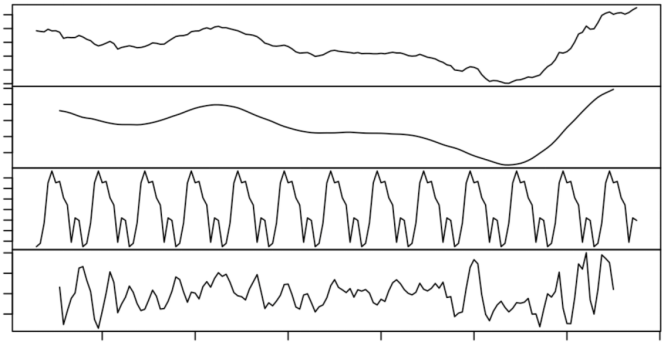
\includegraphics[width=0.8\textwidth]{picture/Decomposition2.png}};
            \node at (2.1,-0.3){\small 2012};
            \node at (3.9,-0.3){\small 2014};
            \node at (5.7,-0.3){\small 2016};
            \node at (7.5,-0.3){\small 2018};
            \node at (9.35,-0.3){\small 2020};
            \node at (11.3,-0.3){\small 2022};
            \node at (13.2,-0.3){\small 2024};
            \node at (6.4,-1){\textbf{Time}};

            \node at(-0.2,0.6)[rotate=90]{\small -0.2}; 
            \node at(-0.2,1.4)[rotate=90]{\small 0.2}; 
            \node at(-0.2,2)[rotate=90]{\small -0.06}; 
            \node at(-0.2,2.95)[rotate=90]{\small 0.02}; 
            \node at(-0.2,3.78)[rotate=90]{\small 1}; 
            \node at(-0.2,4.4)[rotate=90]{\small 3}; 
            \node at(-0.2,5)[rotate=90]{\small 5};
             \node at(-0.2,5.15)[rotate=90]{\small 0};
             \node at(-0.2,5.65)[rotate=90]{\small 2};
              \node at(-0.2,6.22)[rotate=90]{\small 4};
           \node at(-1,3.5)[rotate=90]{\textbf{Random Seasonal Trend Observed}};
        \end{tikzpicture}
    \caption{Decomposition of additive time series}
  \label{D2}
\end{figure}

% \begin{figure}[H]
%     \centering
%     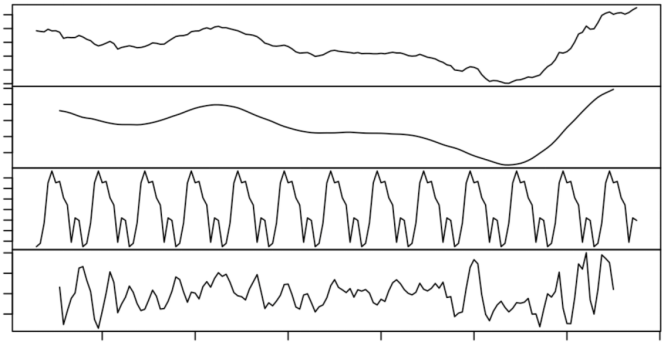
\includegraphics[width=0.8\textwidth]{picture/Decomposition2.png}
%   \vspace{20pt}\caption{\hyperref[Decomposition2]{Decomposition of additive time series}}
%  %   \label{Decomposition}

%     \begin{picture}(0,0)
%         \put(0.37\textwidth,0.097\textwidth){\makebox(0,0)[lt]{\small{{2024}}}}
%         \put(0.26\textwidth,0.097\textwidth){\makebox(0,0)[lt]{\small{{2022}}}}
%         \put(0.15\textwidth,0.097\textwidth){\makebox(0,0)[lt]{\small{{2020}}}}
%         \put(0.04\textwidth,0.097\textwidth){\makebox(0,0)[lt]{\small{{2018}}}}
%         \put(-0.075\textwidth,0.097\textwidth){\makebox(0,0)[lt]{\small{{2016}}}}
%         \put(-0.19\textwidth,0.097\textwidth){\makebox(0,0)[lt]{\small{{2014}}}}
%         \put(-0.3\textwidth,0.097\textwidth){\makebox(0,0)[lt]{\small{{2012}}}}

%         \put(-0.43\textwidth,0.16\textwidth){\makebox(0,0)[lt]{\rotatebox{90}{\small{-0.2}}}}
%         \put(-0.43\textwidth,0.205\textwidth){\makebox(0,0)[lt]{\rotatebox{90}{\small{0.2}}}}
%         \put(-0.43\textwidth,0.25\textwidth){\makebox(0,0)[lt]{\rotatebox{90}{\small{-0.06}}}}
%         \put(-0.43\textwidth,0.306\textwidth){\makebox(0,0)[lt]{\rotatebox{90}{\small{0.02}}}}
%         \put(-0.43\textwidth,0.348\textwidth){\makebox(0,0)[lt]{\rotatebox{90}{\small{1}}}}
%         \put(-0.43\textwidth,0.383\textwidth){\makebox(0,0)[lt]{\rotatebox{90}{\small{3}}}}
%         \put(-0.43\textwidth,0.425\textwidth){\makebox(0,0)[lt]{\rotatebox{90}{\small{50}}}}
%         \put(-0.43\textwidth,0.46\textwidth){\makebox(0,0)[lt]{\rotatebox{90}{\small{2}}}}
%         \put(-0.43\textwidth,0.49\textwidth){\makebox(0,0)[lt]{\rotatebox{90}{\small{4}}}}

%         \put(-0.02\textwidth,0.07\textwidth){\makebox(0,0)[lt]{\textbf{Time}}}
%         \put(-0.47\textwidth,0.47\textwidth){\makebox(0,0)[lt]{\rotatebox{90}{\textbf{Random Seasonal Trend Observed}}}}

%     \end{picture}
% \end{figure}

The two-year period swap rate data also has a similar result to the one-year period swap rate data. From Figure 5, the time series will obtain a random, volatile component. Furthermore, Figure 4 shows that the data hinting at seasonality and the ADF test shows that the p-value surpasses the significance level of 0.05 and the ADF statistic is greater than any of the established critical values; we have no compelling reason to reject the null hypothesis and the time series is nonstationary. 

\subsubsection{The test of 1 year interbank rate}


%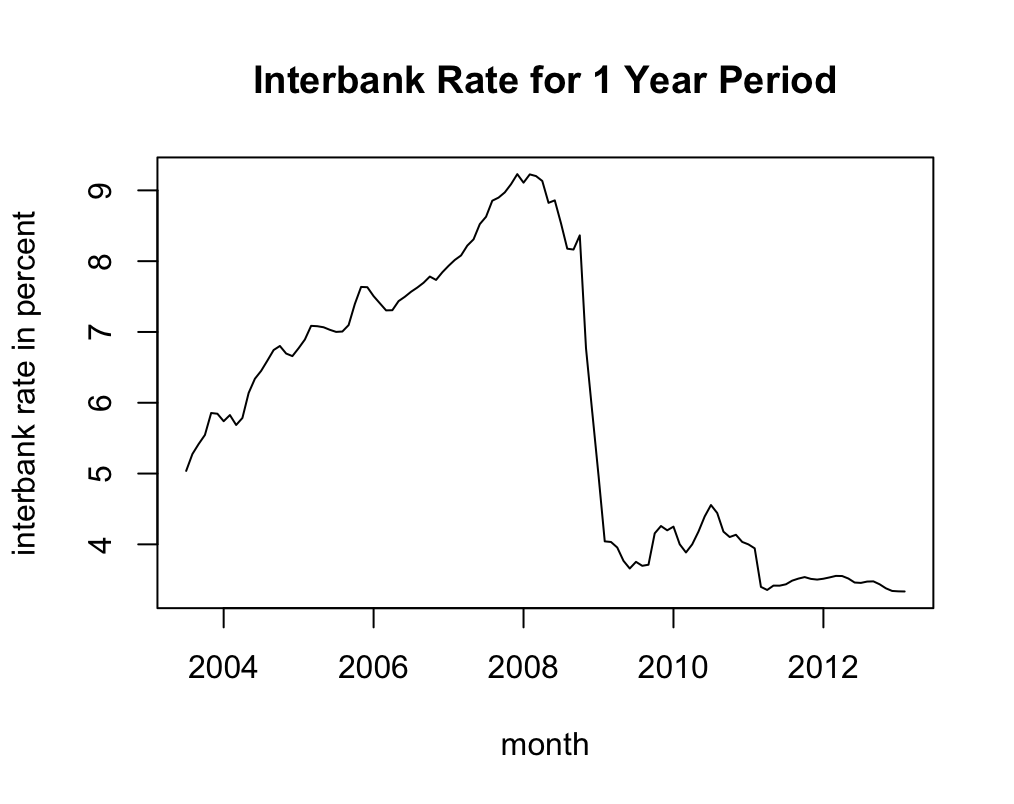
\includegraphics[scale =0.45]{picture/in.png}

\begin{figure}[H]
    \centering
        \begin{tikzpicture}[global scale = 1]
            \node[anchor=south west,inner sep=0] at (0,0) {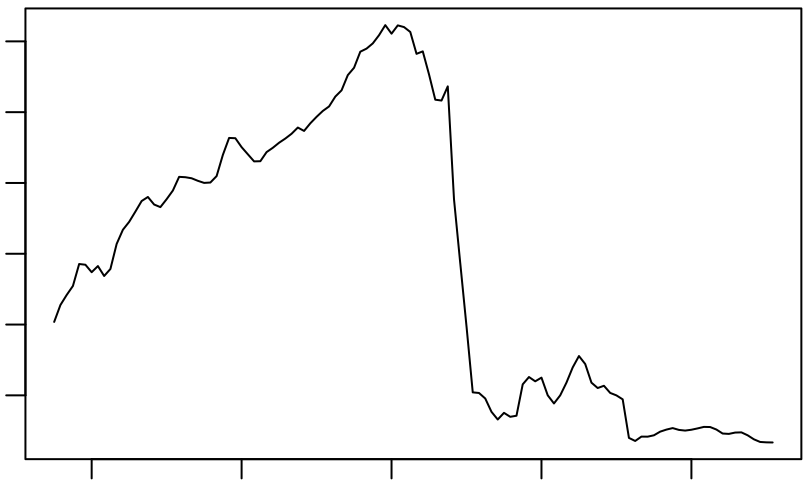
\includegraphics[width=0.8\textwidth]{picture/in_.png}};
    \node at(11.3,-0.3){\small 2012};     
    \node at(8.9,-0.3){\small 2010}; 
    \node at(6.4,-0.3){\small 2008}; 
    \node at(4,-0.3){\small 2006}; 
    \node at(1.5,-0.3){\small 2004}; 
    \node at(6.4,-1){\small month};   
 
    \node at(-0.3,1.5)[rotate=90]{\small 4};   
    \node at(-0.3,2.6)[rotate=90]{\small 5};    
    \node at(-0.3,3.8)[rotate=90]{\small 6};   
    \node at(-0.3,4.9)[rotate=90]{\small 7};    
    \node at(-0.3,6)[rotate=90]{\small 8};  
    \node at(-0.3,7.3)[rotate=90]{\small 9}; 
    \node at(-1,4)[rotate=90]{\small Interbank Rate in Percent};   
    
        \end{tikzpicture}
    \caption{Interbank Rate for 1 Year Period}
    \label{Interbankrate}
\end{figure}


% 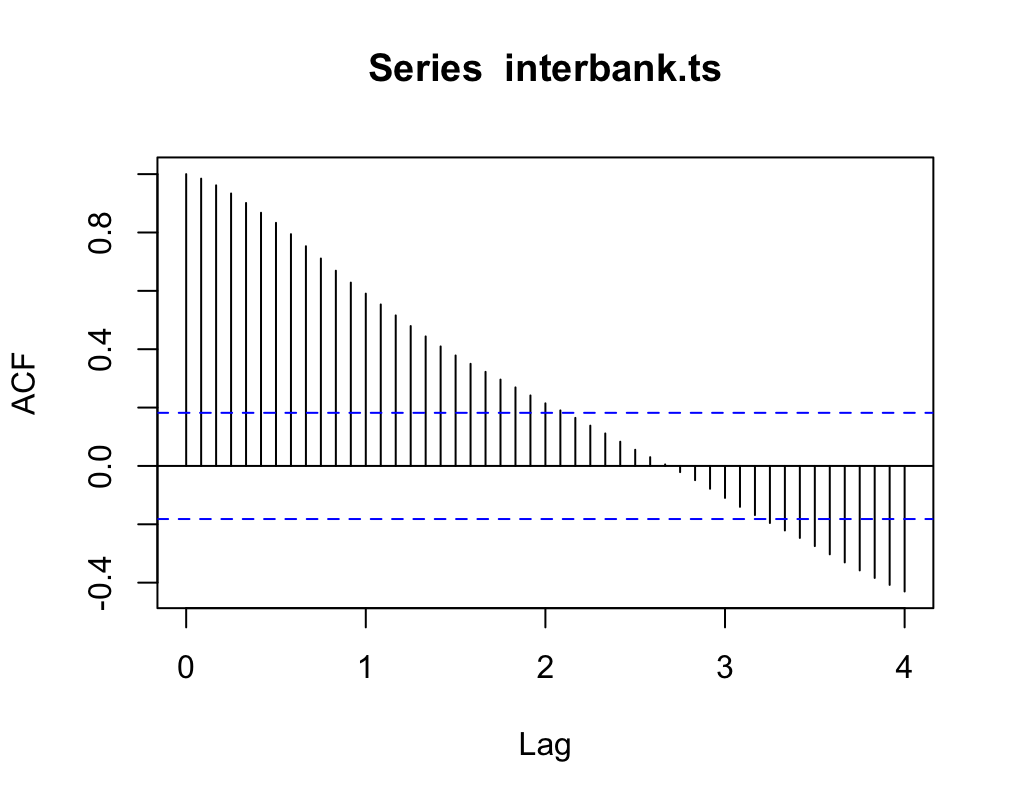
\includegraphics[scale =0.225]{picture/in1.png}
% 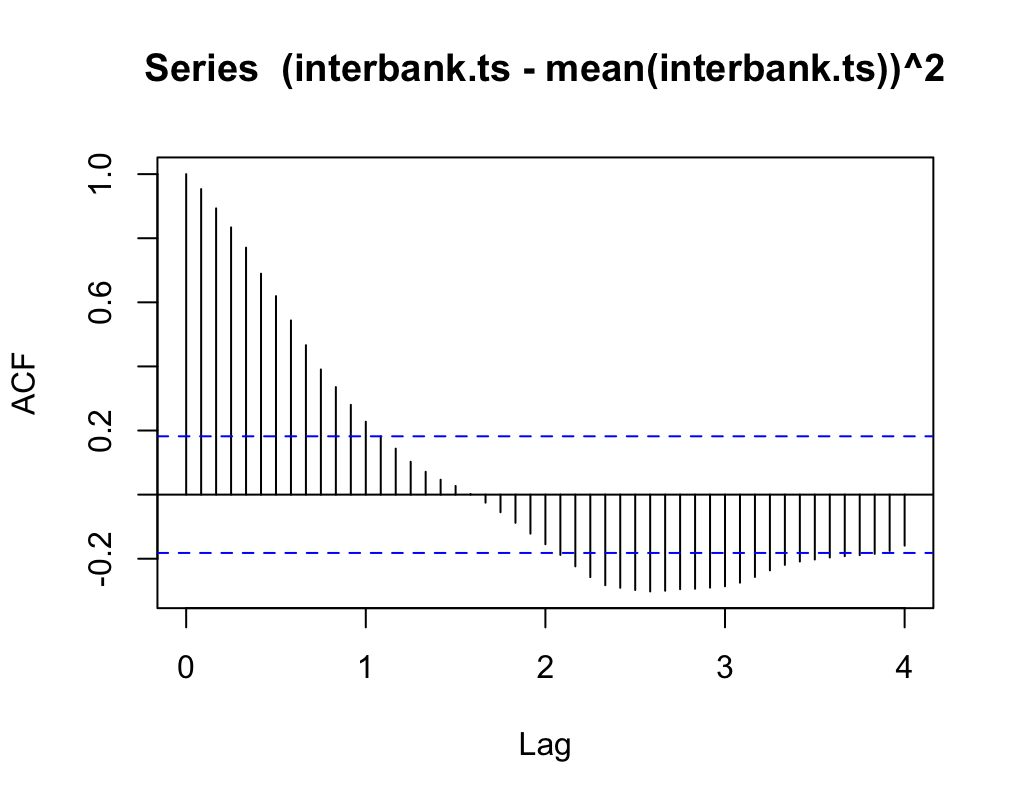
\includegraphics[scale =0.225]{picture/in2.png}

\begin{figure}[H]
    \centering
        \begin{tikzpicture}[global scale = 1]
            \node[anchor=south west,inner sep=0] at (0,0) {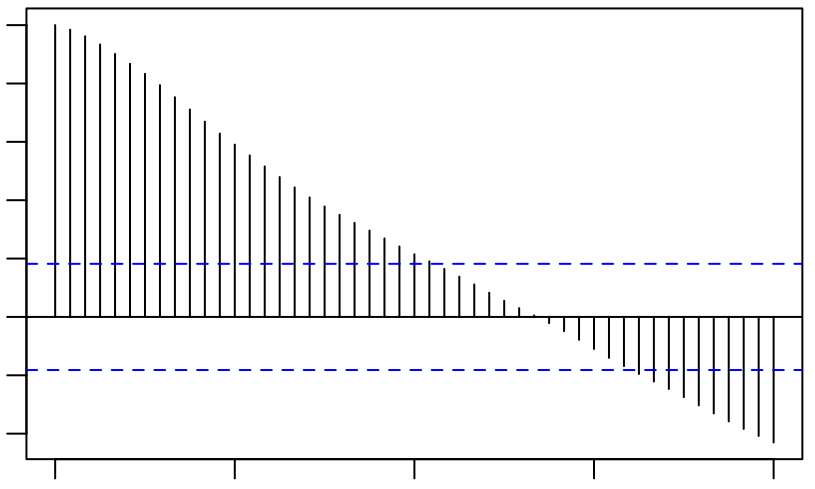
\includegraphics[width=0.3\textwidth]{picture/in1_.png}};
    \node at(0.35,-0.15){\small 0};
    \node at(1.423,-0.15){\small 1};     
    \node at(2.52,-0.15){\small 2};
    \node at(3.603,-0.15){\small 3};   
    \node at(4.7,-0.15){\small 4};
    \node at(2.63,-0.8){\small Lag};
    \node at(2.63,3.5){\small \textbf{Series Interbank.ts}};

    \node at(-0.2,0.3)[rotate=90]{\small -0.4};        
    \node at(-0.2,1.05)[rotate=90]{\small 0.0};  
    \node at(-0.2,1.8)[rotate=90]{\small 0.4};  
    \node at(-0.2,2.5)[rotate=90]{\small 0.8};  
    \node at(-1,1.2)[rotate=90]{\small ACF};        

    
            \node[anchor=south west,inner sep=0] at (7,0) {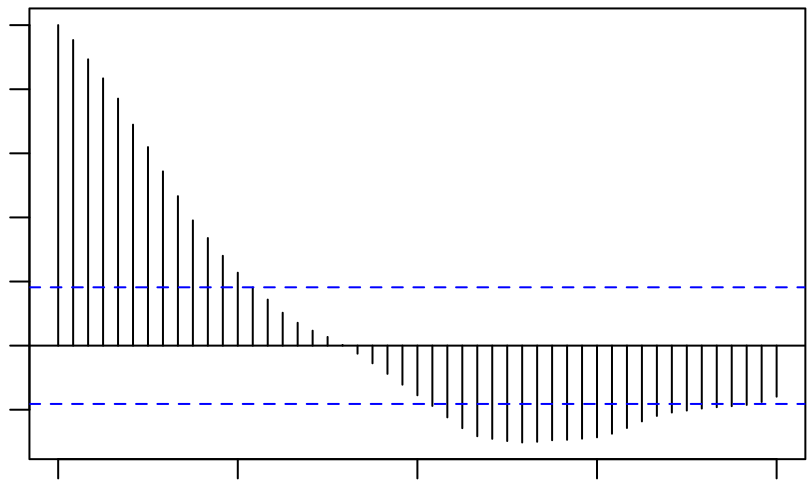
\includegraphics[width=0.3\textwidth]{picture/in2_.png}};
            \node at(9.5,3.5){\small \textbf{ Series (Interbank.ts-mean(Interbank.ts))$^2$}};

    \node at(7.05+0.35,-0.15){\small 0};
    \node at(7.05+1.423,-0.15){\small 1};     
    \node at(7.05+2.52,-0.15){\small 2};
    \node at(7.05+3.603,-0.15){\small 3};   
    \node at(7.05+4.7,-0.15){\small 4};
    \node at(7.05+2.63,-0.8){\small Lag};

    \node at(7+-0.2,0.4)[rotate=90]{\small -0.2};        
    \node at(7+-0.2,1.2)[rotate=90]{\small 0.2};  
    \node at(7+-0.2,2)[rotate=90]{\small 0.6};  
    \node at(7+-0.2,2.7)[rotate=90]{\small 1.0};  
    \node at(7+-1,1.2)[rotate=90]{\small ACF};   
        \end{tikzpicture}
    \caption{}
   \label{I7}
\end{figure}





%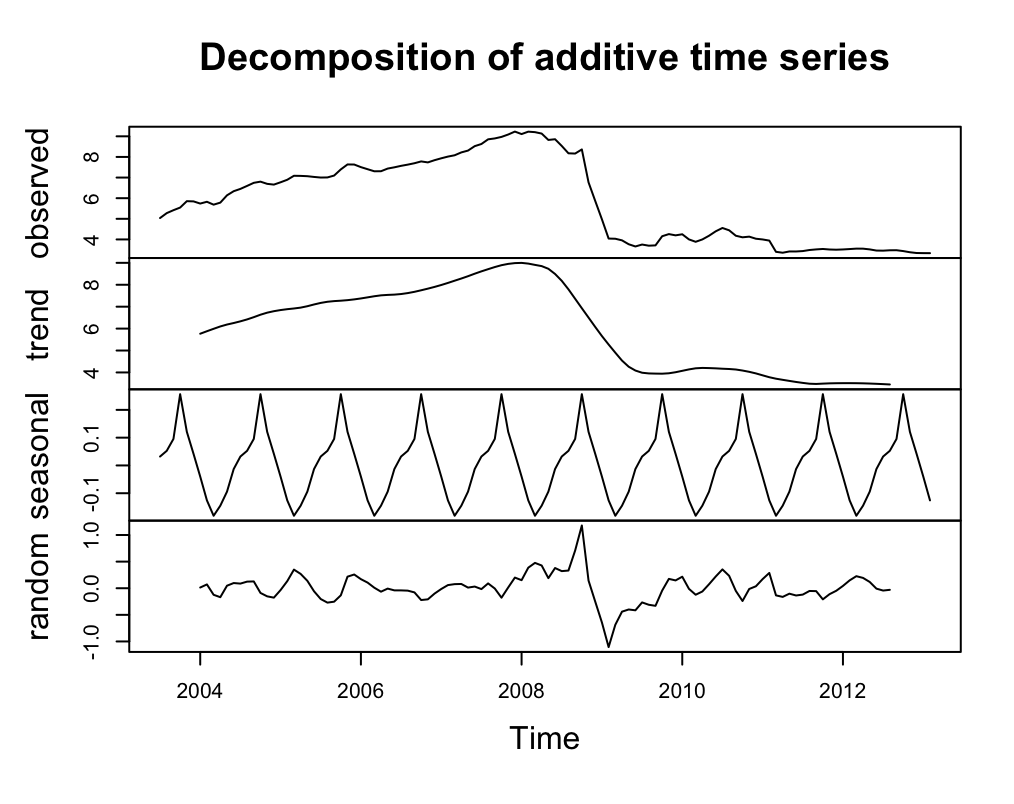
\includegraphics[scale =0.45]{picture/in3.png}
\tikzset{global scale/.style={
    scale=#1,
    every node/.append style={scale=#1}
  }
}
\begin{figure}[H]
    \centering
        \begin{tikzpicture}[global scale = 1]
            \node[anchor=south west,inner sep=0] at (0,0) {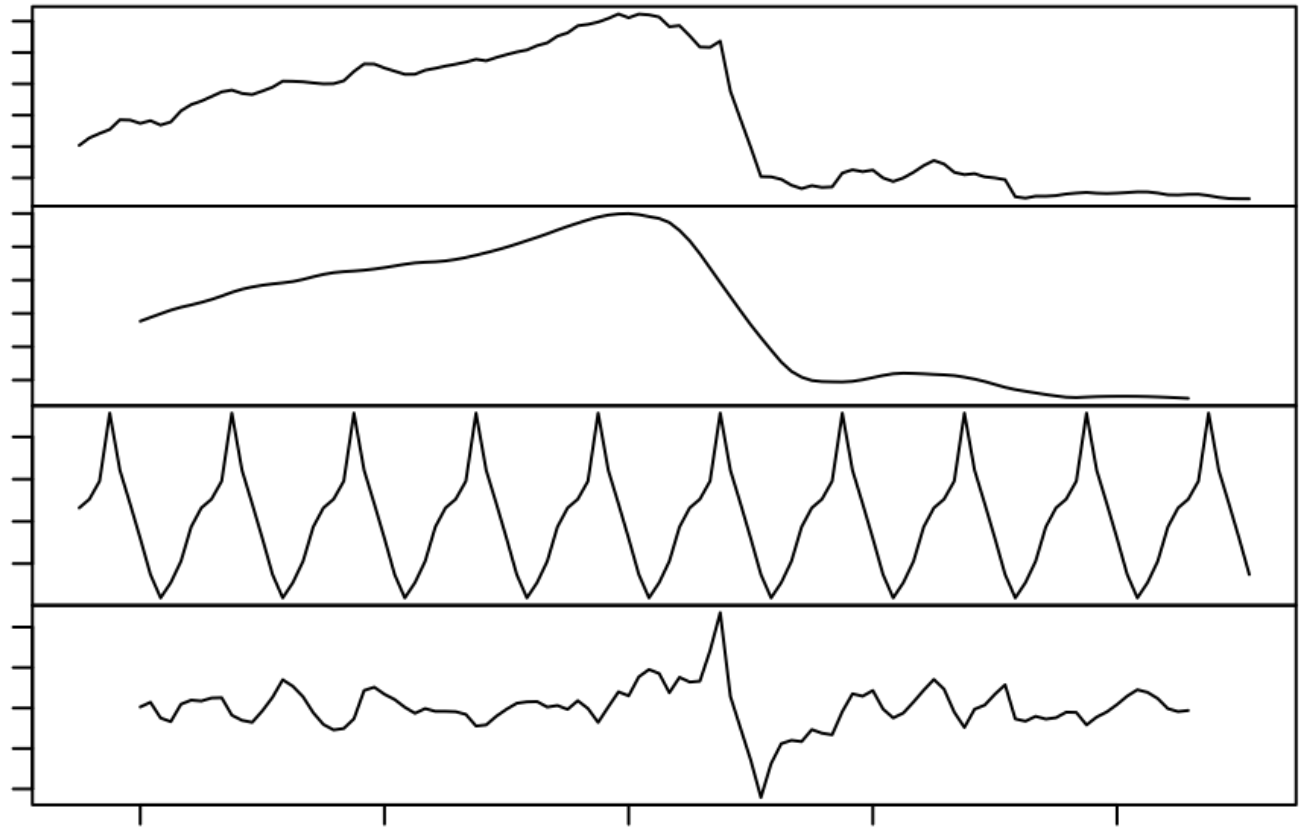
\includegraphics[width=0.8\textwidth]{picture/in3_.png}};
            \node at (1.45,-0.3){\small 2004};
            \node at (3.9,-0.3){\small 2006};
            \node at (6.3,-0.3){\small 2008};
            \node at (8.8,-0.3){\small 2010};
            \node at (11.2,-0.3){\small 2012};

            \node at (6.4,-1){\textbf{Time}};

            \node at(-0.2,0.42)[rotate=90]{\small -1.0}; 
            \node at(-0.2,1.2)[rotate=90]{\small 0.0}; 
            \node at(-0.2,2)[rotate=90]{\small 1.0}; 
            \node at(-0.2,2.7)[rotate=90]{\small -0.1}; 
            \node at(-0.2,3.5)[rotate=90]{\small 0.1}; 
            \node at(-0.2,4.55)[rotate=90]{\small 4}; 
            \node at(-0.2,5.2)[rotate=90]{\small 6};
            \node at(-0.2,5.85)[rotate=90]{\small 8};
             \node at(-0.2,6.55)[rotate=90]{\small 4};
             \node at(-0.2,7.2)[rotate=90]{\small 6};
              \node at(-0.2,7.845)[rotate=90]{\small 8};
           \node at(-1,4)[rotate=90]{\textbf{Random Seasonal Trend Observed}};
        \end{tikzpicture}
    \caption{Decomposition of additive time series}
    \label{in3}
\end{figure}


The one-year period interbank rates data also has a similar result to the one-year swap rate data and two-year swap rate data. From Figure 8, the time series will obtain a random, volatile component. Furthermore, Figure 7 shows that the data hinting at seasonality and the ADF test shows that the p-value surpasses the significance level of 0.05 and the ADF statistic is greater than any of the established critical values; we have no compelling reason to reject the null hypothesis and the time series is nonstationary. 





\subsection{Predicting Yield Rates Using Swap Rates}


\begin{figure}[H]
    \centering
        \begin{tikzpicture}[global scale = 1]
            \node[anchor=south west,inner sep=0] at (0,0) {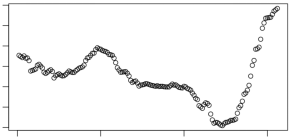
\includegraphics[width=0.3\textwidth]{picture/Swap2_1.png}};
    \node at(0.35,-0.15){\small 0};
    \node at(1.74,-0.15){\small 50};     
    \node at(3.2,-0.15){\small 100};
    \node at(4.65,-0.15){\small 150};   
    \node at(2.7,-0.8){\small month};
    \node at(2.63,2.8){\textbf{\footnotesize Swap Rate for 1 Year Period}};

    \node at(-0.2,0.2)[rotate=90]{\small 0};    
       \node at(-0.2,0.55)[rotate=90]{\small 1}; 
    \node at(-0.2,0.9)[rotate=90]{\small 2};  
    \node at(-0.2,1.25)[rotate=90]{\small 3};
    \node at(-0.2,1.6)[rotate=90]{\small 4};  
    \node at(-0.2,1.95)[rotate=90]{\small 5};
    \node at(-0.2,2.3)[rotate=90]{\small 6};  
    \node at(-1,1.2)[rotate=90]{\small Swap Rate in Percent};        

    
            \node[anchor=south west,inner sep=0] at (7,0) {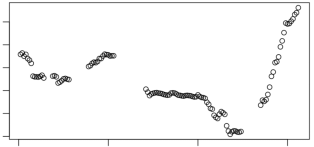
\includegraphics[width=0.3\textwidth]{picture/Yields.png}};
            \node at(9.5,2.8){\textbf{\footnotesize Yields Rate for 1 Year Period}};

    \node at(7+0.35,-0.15){\small 0};
    \node at(7+1.74,-0.15){\small 50};     
    \node at(7+3.2,-0.15){\small 100};
    \node at(7+4.65,-0.15){\small 150};   
    \node at(7+2.7,-0.8){\small Month};


     \node at(7-0.2,0.2)[rotate=90]{\small 0};    
       \node at(7+-0.2,0.55)[rotate=90]{\small 1}; 
    \node at(7+-0.2,0.9)[rotate=90]{\small 2};  
    \node at(7+-0.2,1.25)[rotate=90]{\small 3};
    \node at(7+-0.2,1.6)[rotate=90]{\small 4};  
    \node at(7+-0.2,1.95)[rotate=90]{\small 5};

     \node at(6,1.2)[rotate=90]{\small Yields Rate in Percent};   
        \end{tikzpicture}
    \caption{}
   \label{Swap21}
\end{figure}

\subsubsection{Correlation Between Swap and Yield Rates}

We initiated our analysis by graphing the trends between the swap and yield rates. A visual inspection suggests a potential correlation. This observation led us to employ regression using data from both the yield and swap rates. The following regression model was proposed:
\[Yield\_1year_{i}=c+\beta \cdot Swap\_rate\_1year_{i}+\epsilon_{i}\]

\begin{lstlisting}
Call:
 lm(formula  =  data$bond_closing_yields_1year ~data$Swap_rates_1year)

Residuals:
     Min      1 Q    Median       3Q      Max  
-0.34417  -0.06211 -0.02351  0.05513  0.42781


Coefficients:
                        Estimate Std. Error t value Pr(>|t|)
(Intercept)            -0.047444   0.027415  -1.731   0.0863 .
data$Swap_rates_1year   0.936676   0.009457  99.050   <2 e-16 *** 
---
Signif. codes: 0 '* * *', 0.001 '* *', 0.01 '*', 0.05 '.', 0.1  '' 1
Residual standard error: 0.1328 on 113 degrees of freedom 
  (41 observations deleted due to missingness)
Multiple R-squared: 0.9886,  Adjusted R-squared: 0.9885
F-statistic: 9811 on 1 and 113 DF, p-value: < 2.2e-16    
\end{lstlisting}

\subsubsection{Omitted Variable Bias}
Though the model appeared to be significant, closer scrutiny of the one-year yield rate revealed gaps in the data for specific years. Relying solely on simple linear regression for prediction in such cases can lead to omitted variable bias. This necessitates the exploration of alternative, more reliable methods. The issue of missing data persisted when considering the two-year period.


\begin{lstlisting}
Call:
lm(formula  =  data$bond_closing_yields_2year ~ data$Swap_rates_2year)

Residuals:
      Min        1Q    Median       3Q      Max  
 -0.42686  -0.10933  -0.01985  0.06238  0.54959
 
Coefficients:
                        Estimate Std. Error t value Pr(>|t|)
(Intercept)             -0.13826    0.03648   -3.79 0.000229 *** 
data$Swap_rates_2year    0.96271    0.01245   77.33 <2 e-16 *** 

Residual standard error: 0.1628 on 130 degrees of freedom
(24 observations deleted due to missingness)
Multiple R-squared: 0.9787,  Adjusted R-squared: 0.9786
F-statistic: 5980 on 1 and 130 DF, p-value: < 2.2e-16    
\end{lstlisting}





\begin{figure}[H]
    \centering
        \begin{tikzpicture}[global scale = 1]
            \node[anchor=south west,inner sep=0] at (0,0) {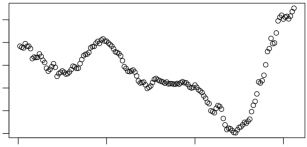
\includegraphics[width=0.3\textwidth]{picture/Swap3_1.png}};
    \node at(0.35,-0.15){\small 0};
    \node at(1.74,-0.15){\small 50};     
    \node at(3.2,-0.15){\small 100};
    \node at(4.65,-0.15){\small 150};   
    \node at(2.7,-0.8){\small month};
    \node at(2.6,2.8){\textbf{\footnotesize Swap Rate for 2 Year Period}};

    \node at(-0.2,0.2)[rotate=90]{\small 0};    
       \node at(-0.2,0.6)[rotate=90]{\small 1}; 
    \node at(-0.2,0.95)[rotate=90]{\small 2};  
    \node at(-0.2,1.35)[rotate=90]{\small 3};
    \node at(-0.2,1.72)[rotate=90]{\small 4};  
    \node at(-0.2,2.1)[rotate=90]{\small 5};
    \node at(-1,1.2)[rotate=90]{\small Swap Rate in Percent};        

    
            \node[anchor=south west,inner sep=0] at (7,0) {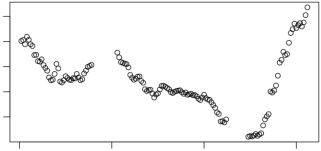
\includegraphics[width=0.3\textwidth]{picture/Yield3_2.png}};
            \node at(9.5,2.8){\textbf{\footnotesize Yields Rate for 2 Year Period}};

    \node at(7+0.35,-0.15){\small 0};
    \node at(7+1.74,-0.15){\small 50};     
    \node at(7+3.2,-0.15){\small 100};
    \node at(7+4.65,-0.15){\small 150};   
    \node at(7+2.7,-0.8){\small month};


     \node at(7-0.2,0.2+0.35)[rotate=90]{\small 1};    
       \node at(7+-0.2,0.55+0.36)[rotate=90]{\small 2}; 
    \node at(7+-0.2,0.9+0.41)[rotate=90]{\small 3};  
    \node at(7+-0.2,1.25+0.43)[rotate=90]{\small 4};
    \node at(7+-0.2,1.6+0.49)[rotate=90]{\small 5};  


     \node at(6,1.2)[rotate=90]{\small Yields Rate in Percent};   
        \end{tikzpicture}
    \caption{}
    \label{Swap31}
\end{figure}


\subsection{Machine Learning – The Random Forest Model}
Random Forest is an ensemble learning technique widely used for both classification and regression tasks.\footnote{\cite{Boehmke_Greenwell_2020}} It operates by constructing numerous decision trees during the training phase and then produces the mode of the classes (for classification) or the mean prediction (for regression) of the individual trees when provided with an input.\footnote{\cite{breiman2001random}}  In our study, we trained the model using swap rate data to predict yield data.

One of the principal advantages of the Random Forest model is its foundation on multiple decision trees. Every tree is trained on a unique, randomly chosen subset of the data and offers its predictions. The model then compiles these predictions to yield a final outcome. This method leverages bagging (bootstrap aggregation) to bolster the model's robustness. When each decision tree is trained, a random data sample is chosen with replacement. Furthermore, Random Forest introduces an element of randomness during node splitting. Instead of selecting the best feature from all available ones during this process, it chooses from a random subset, leading to a diverse tree ensemble. This design helps in mitigating overfitting and maintains data accuracy even in the presence of missing values.\footnote{\cite{hastie2001elements}}

After the data training:
\begin{figure}[H]
    \centering
        \begin{tikzpicture}[global scale = 1]
            \node[anchor=south west,inner sep=0] at (0,0) {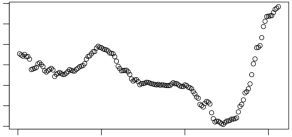
\includegraphics[width=0.3\textwidth]{picture/a_Swap1_1.png}};
    \node at(0.35,-0.15){\small 0};
    \node at(1.74,-0.15){\small 50};     
    \node at(3.2,-0.15){\small 100};
    \node at(4.65,-0.15){\small 150};   
    \node at(2.7,-0.8){\small month};
    \node at(2.63,2.8){\textbf{\footnotesize Swap Rate for 1 Year Period}};

    \node at(-0.2,0.2)[rotate=90]{\small 0};    
       \node at(-0.2,0.55)[rotate=90]{\small 1}; 
    \node at(-0.2,0.9)[rotate=90]{\small 2};  
    \node at(-0.2,1.25)[rotate=90]{\small 3};
    \node at(-0.2,1.6)[rotate=90]{\small 4};  
    \node at(-0.2,1.95)[rotate=90]{\small 5};
    \node at(-0.2,2.3)[rotate=90]{\small 6};  
    \node at(-1,1.2)[rotate=90]{\small Swap Rate in Percent};        

    
            \node[anchor=south west,inner sep=0] at (7,0) {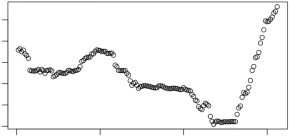
\includegraphics[width=0.3\textwidth]{picture/a_Yields.png}};
            \node at(9.5,2.8){\textbf{\footnotesize Yields Rate for 1 Year Period}};

    \node at(7+0.35,-0.15){\small 0};
    \node at(7+1.74,-0.15){\small 50};     
    \node at(7+3.2,-0.15){\small 100};
    \node at(7+4.65,-0.15){\small 150};   
    \node at(7+2.7,-0.8){\small Month};


     \node at(7-0.2,0.2)[rotate=90]{\small 0};    
       \node at(7+-0.2,0.55)[rotate=90]{\small 1}; 
    \node at(7+-0.2,0.9)[rotate=90]{\small 2};  
    \node at(7+-0.2,1.25)[rotate=90]{\small 3};
    \node at(7+-0.2,1.6)[rotate=90]{\small 4};  
    \node at(7+-0.2,1.95)[rotate=90]{\small 5};

     \node at(6,1.2)[rotate=90]{\small Yields Rate in Percent};   
        \end{tikzpicture}
    \caption{}
   \label{Swap41}
\end{figure}



\begin{figure}[H]
    \centering
        \begin{tikzpicture}[global scale = 1]
            \node[anchor=south west,inner sep=0] at (0,0) {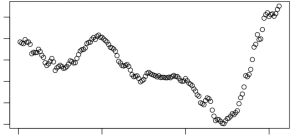
\includegraphics[width=0.3\textwidth]{picture/a_Swap2_1.png}};
    \node at(0.35,-0.15){\small 0};
    \node at(1.74,-0.15){\small 50};     
    \node at(3.2,-0.15){\small 100};
    \node at(4.65,-0.15){\small 150};   
    \node at(2.7,-0.8){\small month};
    \node at(2.63,2.8){\hyperref[Swap51]{\textbf{\footnotesize Swap Rate for 2 Year Period}}};

    \node at(-0.2,0.2)[rotate=90]{\small 0};    
       \node at(-0.2,0.6)[rotate=90]{\small 1}; 
    \node at(-0.2,0.95)[rotate=90]{\small 2};  
    \node at(-0.2,1.35)[rotate=90]{\small 3};
    \node at(-0.2,1.72)[rotate=90]{\small 4};  
    \node at(-0.2,2.1)[rotate=90]{\small 5};
    \node at(-1,1.2)[rotate=90]{\small Swap Rate in Percent};        

    
            \node[anchor=south west,inner sep=0] at (7,0) {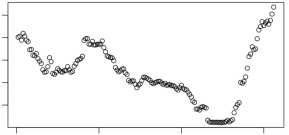
\includegraphics[width=0.3\textwidth]{picture/a_Yields2_2.png}};
            \node at(9.5,2.8){ \hyperref[Yields52]{\textbf{\footnotesize Yields Rate for 2 Year Period}}};

    \node at(7+0.35,-0.15){\small 0};
    \node at(7+1.74,-0.15){\small 50};     
    \node at(7+3.2,-0.15){\small 100};
    \node at(7+4.65,-0.15){\small 150};   
    \node at(7+2.7,-0.8){\small month};


     \node at(7-0.2,0.2+0.35)[rotate=90]{\small 1};    
       \node at(7+-0.2,0.55+0.36)[rotate=90]{\small 2}; 
    \node at(7+-0.2,0.9+0.41)[rotate=90]{\small 3};  
    \node at(7+-0.2,1.25+0.43)[rotate=90]{\small 4};
    \node at(7+-0.2,1.6+0.49)[rotate=90]{\small 5};  


     \node at(6,1.2)[rotate=90]{\small Yields Rate in Percent};   
        \end{tikzpicture}
    \caption{}
  %  \label{Series2}
\end{figure}


\subsection{Test of filled variable}
After we found the missing data, we now examine the completed data to ensure that they have the same data characteristics

\subsubsection{1 year yield rate}

\begin{lstlisting}
        Augmented Dickey-Fuller Test
        
data: Yield.ts
Dickey-Fuller = -0.14344, Lag order = 5, p -value = 0.99 
alternative hypothesis: stationary    
\end{lstlisting}


\begin{figure}[H]
    \centering
        \begin{tikzpicture}[global scale = 1]
            \node[anchor=south west,inner sep=0] at (0,0) {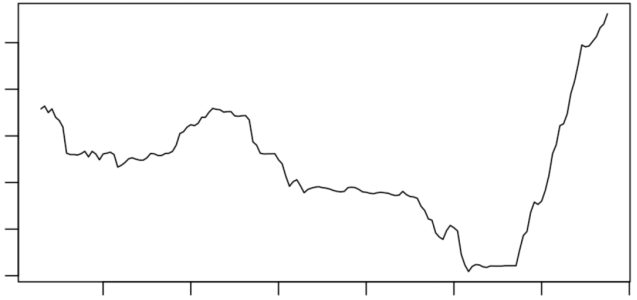
\includegraphics[width=0.8\textwidth]{picture/Yield_4.png}};
    \node at(13.15,-0.3){\small 2024};
    \node at(11.3,-0.3){\small 2022};     
    \node at(9.5,-0.3){\small 2020}; 
    \node at(7.6,-0.3){\small 2018}; 
    \node at(5.83,-0.3){\small 2016}; 
    \node at(4.0,-0.3){\small 2014}; 
    \node at(2.2,-0.3){\small 2012};    
    \node at(6.7,-1){\small month};   

    \node at(-0.3,0.5)[rotate=90]{\small 0};    
    \node at(-0.3,1.5)[rotate=90]{\small 1};   
    \node at(-0.3,2.5)[rotate=90]{\small 2};    
    \node at(-0.3,3.4)[rotate=90]{\small 3};   
    \node at(-0.3,4.3)[rotate=90]{\small 4};    
    \node at(-0.3,5.36)[rotate=90]{\small 5};   
    \node at(-1,3)[rotate=90]{\small Yield Rate in Percent};   
    
     \end{tikzpicture}
    \caption{{Yield Rate for 1 Year Period}}
   \label{Yields6}
\end{figure}




\begin{figure}[H]
    \centering
        \begin{tikzpicture}[global scale = 1]
            \node[anchor=south west,inner sep=0] at (0,0) {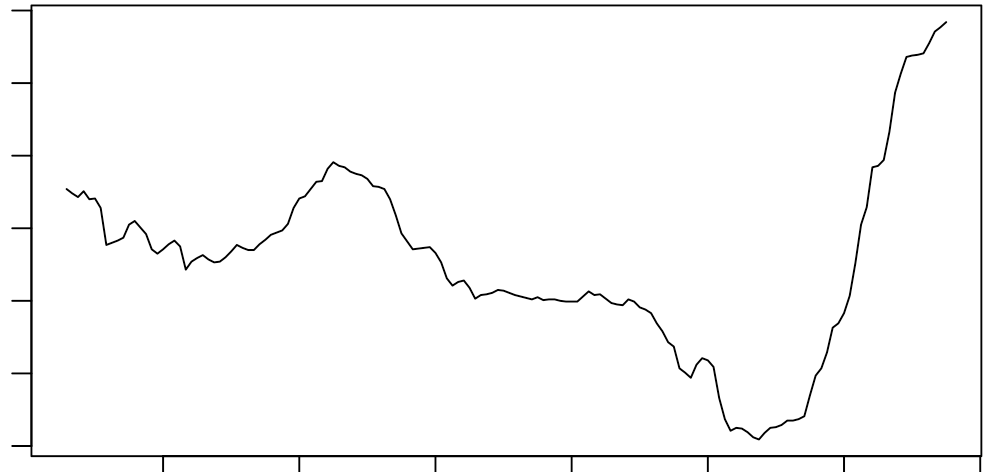
\includegraphics[width=0.8\textwidth]{picture/1231.png}};
    \node at(13,-0.3){\small 2024};
    \node at(11.15,-0.3){\small 2022};     
    \node at(9.4,-0.3){\small 2020}; 
    \node at(7.58,-0.3){\small 2018}; 
    \node at(5.8,-0.3){\small 2016}; 
    \node at(3.98,-0.3){\small 2014}; 
    \node at(2.2,-0.3){\small 2012};    
    \node at(6.7,-1){\small month};   


    

    \node at(-0.3,0.5)[rotate=90]{\small 0};    
    \node at(-0.3,1.5)[rotate=90]{\small 1};   
    \node at(-0.3,2.5)[rotate=90]{\small 2};    
    \node at(-0.3,3.4)[rotate=90]{\small 3};   
    \node at(-0.3,4.34)[rotate=90]{\small 4};    
    \node at(-0.3,5.36)[rotate=90]{\small 5}; 
    \node at(-1,3)[rotate=90]{\small Swap Rate in Percent};   
    
        \end{tikzpicture}
    \caption{Swap Rate for 1 Year Period}
   \label{Swap6}
\end{figure}

\begin{figure}[H]
    \centering
        \begin{tikzpicture}[global scale = 1]
            \node[anchor=south west,inner sep=0] at (0,0) {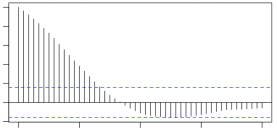
\includegraphics[width=0.3\textwidth]{picture/Series4_1.png}};
    \node at(0.35,-0.15){\small 0};
    \node at(1.46,-0.15){\small 1};     
    \node at(2.55,-0.15){\small 2};
    \node at(3.65,-0.15){\small 3};   
    \node at(4.7,-0.15){\small 4};
    \node at(2.63,-0.8){\small Lag};
    \node at(2.63,2.8){\textbf{\footnotesize Series Yield.ts}};

    \node at(-0.2,0.2)[rotate=90]{\small -0.2};        
    \node at(-0.2,0.9)[rotate=90]{\small 0.2};  
    \node at(-0.2,1.6)[rotate=90]{\small 0.6};  
    \node at(-0.2,2.3)[rotate=90]{\small 1.0};  
    \node at(-1,1.2)[rotate=90]{\small ACF};        

    
            \node[anchor=south west,inner sep=0] at (7,0) {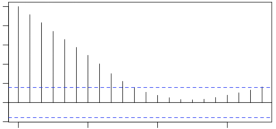
\includegraphics[width=0.3\textwidth]{picture/Series4_2.png}};
            \node at(9.5,2.8){\textbf{\footnotesize Series (Yield.ts-mean(Yield.ts))$^2$}};

    \node at(7+0.4,-0.15){\small 0.0};     
    \node at(7+1.65,-0.15){\small 0.5};
    \node at(7+2.82,-0.15){\small 1.0};   
    \node at(7+4.15,-0.15){\small 1.5};
    \node at(7+2.63,-0.8){\small Lag};

    \node at(7+-0.2,0.2)[rotate=90]{\small -0.0};        
    \node at(7+-0.2,0.9)[rotate=90]{\small 0.2};  
    \node at(7+-0.2,1.6)[rotate=90]{\small 0.6};  
    \node at(7+-0.2,2.3)[rotate=90]{\small 1.0};  
    \node at(7+-1,1.2)[rotate=90]{\small ACF};   
        \end{tikzpicture}
    \caption{}
    \label{Series71}
\end{figure}


\tikzset{global scale/.style={
    scale=#1,
    every node/.append style={scale=#1}
  }
}
\begin{figure}[H]
    \centering
        \begin{tikzpicture}[global scale = 1]
            \node[anchor=south west,inner sep=0] at (0,0) {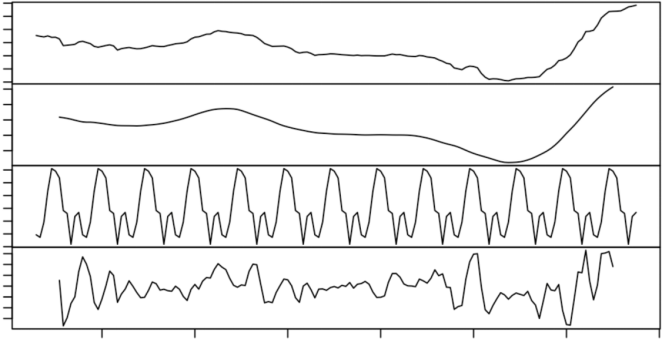
\includegraphics[width=0.8\textwidth]{picture/Decomposition.png}};
            \node at (2.1,-0.3){\small 2012};
            \node at (3.92,-0.3){\small 2014};
            \node at (5.9,-0.3){\small 2016};
            \node at (7.68,-0.3){\small 2018};
            \node at (9.5,-0.3){\small 2020};
            \node at (11.3,-0.3){\small 2022};
            \node at (13.2,-0.3){\small 2024};
            \node at (6.4,-1){\textbf{Time}};

            \node at(-0.2,0.35)[rotate=90]{\small -0.3}; 
            \node at(-0.2,1.25)[rotate=90]{\small 0.1}; 
            \node at(-0.2,1.8)[rotate=90]{\small -0.06}; 
            \node at(-0.2,2.9)[rotate=90]{\small 0.02}; 
            \node at(-0.2,3.75)[rotate=90]{\small 1}; 
            \node at(-0.2,4.35)[rotate=90]{\small 3}; 
            \node at(-0.2,4.95)[rotate=90]{\small 5};
             \node at(-0.2,5.1)[rotate=90]{\small 0};
             \node at(-0.2,5.62)[rotate=90]{\small 2};
              \node at(-0.2,6.15)[rotate=90]{\small 4};
               \node at(-0.2,6.75)[rotate=90]{\small 6};
        \end{tikzpicture}
    \caption{Decomposition of additive time series}
   \label{De2}
\end{figure}

Overall, the 1 year yield data after filling in the missing data and the 1 year swap data have similar trends and seasonality. 1 year yield data is also a non-stationary time series.

Therefore, we have sufficient evidence to believe that the 1 year yield data is reliable.






\subsubsection{For 2 year period}
\begin{lstlisting}
        Augmented Dickey-Fuller Test
        
data: Yield.ts1
Dickey-Fuller = -0.29267, Lag order = 5, -value = 0.9899 
alternative hypothesis: stationary    
\end{lstlisting}




\begin{figure}[H]
    \centering
        \begin{tikzpicture}[global scale = 1]
            \node[anchor=south west,inner sep=0] at (0,0) {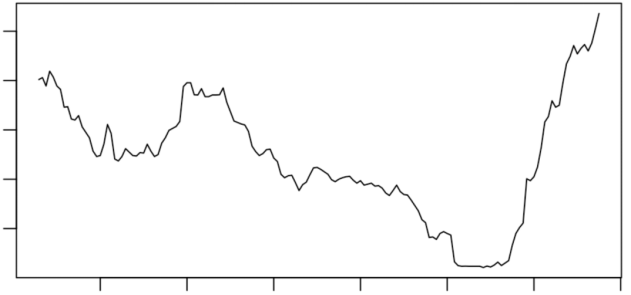
\includegraphics[width=0.8\textwidth]{picture/Yields5.png}};
    \node at(13.1,-0.3){\small 2024};
    \node at(11.3,-0.3){\small 2022};     
    \node at(9.45,-0.3){\small 2020}; 
    \node at(7.6,-0.3){\small 2018}; 
    \node at(5.85,-0.3){\small 2016}; 
    \node at(4,-0.3){\small 2014}; 
    \node at(2.2,-0.3){\small 2012};    
    \node at(6.7,-1){\small month};   

 
    \node at(-0.3,1.4)[rotate=90]{\small 1};   
    \node at(-0.3,2.5)[rotate=90]{\small 2};    
    \node at(-0.3,3.6)[rotate=90]{\small 3};   
    \node at(-0.3,4.7)[rotate=90]{\small 4};    
    \node at(-0.3,5.8)[rotate=90]{\small 5};   
    \node at(-1,3)[rotate=90]{\small Swap Rate in Percent};   
    
        \end{tikzpicture}
    \caption{{Yield rate for 2 Year Period}}
    \label{Yield12}
\end{figure}


\begin{figure}[H]
    \centering
        \begin{tikzpicture}[global scale = 1]
            \node[anchor=south west,inner sep=0] at (0,0) {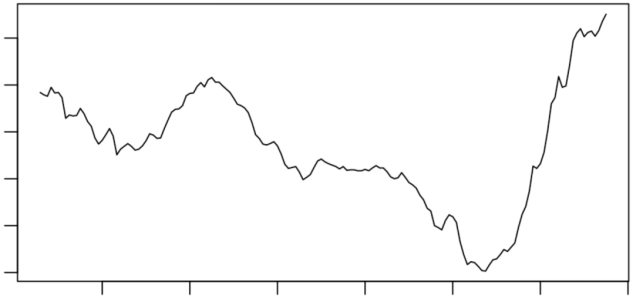
\includegraphics[width=0.8\textwidth]{picture/Swap.png}};
    \node at(13,-0.3){\small 2024};
    \node at(11.2,-0.3){\small 2022};     
    \node at(9.4,-0.3){\small 2020}; 
    \node at(7.6,-0.3){\small 2018}; 
    \node at(5.76,-0.3){\small 2016}; 
    \node at(4,-0.3){\small 2014}; 
    \node at(2.2,-0.3){\small 2012};    
    \node at(6.7,-1){\small Month};   


    

    \node at(-0.3,0.5)[rotate=90]{\small 0};    
    \node at(-0.3,1.5)[rotate=90]{\small 1};   
    \node at(-0.3,2.5)[rotate=90]{\small 2};    
    \node at(-0.3,3.5)[rotate=90]{\small 3};   
    \node at(-0.3,4.5)[rotate=90]{\small 4};    
    \node at(-0.3,5.5)[rotate=90]{\small 5};   
    \node at(-1,3)[rotate=90]{\small Swap Rate in Percent};   
    
        \end{tikzpicture}
    \caption{{Swap Rate for 2 Year Period}}
    \label{Yield_n}
\end{figure}


\begin{figure}[H]
    \centering
        \begin{tikzpicture}[global scale = 1]
            \node[anchor=south west,inner sep=0] at (0,0) {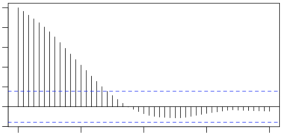
\includegraphics[width=0.3\textwidth]{picture/Series5_1.png}};
    \node at(0.35,-0.15){\small 0};
    \node at(1.43,-0.15){\small 1};     
    \node at(2.54,-0.15){\small 2};
    \node at(3.6,-0.15){\small 3};   
    \node at(4.68,-0.15){\small 4};
    \node at(2.63,-0.8){\small Lag};
    \node at(2.63,2.8){\textbf{Series Yield.ts1}};

    \node at(-0.2,0.2)[rotate=90]{\small -0.2};        
    \node at(-0.2,0.9)[rotate=90]{\small 0.2};  
    \node at(-0.2,1.6)[rotate=90]{\small 0.6};  
    \node at(-0.2,2.3)[rotate=90]{\small 1.0};  
    \node at(-1,1.2)[rotate=90]{\small ACF};        

    
            \node[anchor=south west,inner sep=0] at (7,0) {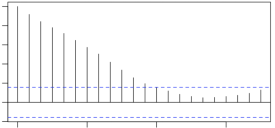
\includegraphics[width=0.3\textwidth]{picture/Series5_2.png}};
            \node at(9.5,2.8){\textbf{Series (Yield.ts1-mean(Yield.ts1))$^2$}};

    \node at(7+0.4,-0.15){\small 0.0};     
    \node at(7+1.6,-0.15){\small 0.5};
    \node at(7+2.85,-0.15){\small 1.0};   
    \node at(7+4.15,-0.15){\small 1.5};
    \node at(7+2.63,-0.8){\small Lag};

    \node at(7+-0.2,0.2)[rotate=90]{\small -0.0};        
    \node at(7+-0.2,0.9)[rotate=90]{\small 0.2};  
    \node at(7+-0.2,1.6)[rotate=90]{\small 0.6};  
    \node at(7+-0.2,2.3)[rotate=90]{\small 1.0};  
    \node at(7+-1,1.2)[rotate=90]{\small ACF};   
        \end{tikzpicture}
    \caption{}
    \label{Series13}
\end{figure}


% \begin{figure}[H]
%     \centering
%     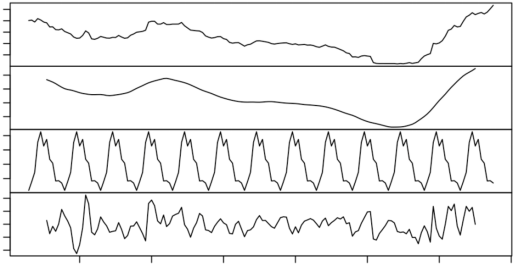
\includegraphics[width=0.8\textwidth]{picture/Decomposition4.png}
%   \vspace{20pt}\caption{\hyperref[Decomposition4]{Decomposition of Additive Time Series}}
%  %   \label{Decomposition}

%     \begin{picture}(0,0)
%         \put(0.365\textwidth,0.097\textwidth){\makebox(0,0)[lt]{\small{{2024}}}}
%         \put(0.25\textwidth,0.097\textwidth){\makebox(0,0)[lt]{\small{{2022}}}}
%         \put(0.145\textwidth,0.097\textwidth){\makebox(0,0)[lt]{\small{{2020}}}}
%         \put(0.03\textwidth,0.097\textwidth){\makebox(0,0)[lt]{\small{{2018}}}}
%         \put(-0.08\textwidth,0.097\textwidth){\makebox(0,0)[lt]{\small{{2016}}}}
%         \put(-0.19\textwidth,0.097\textwidth){\makebox(0,0)[lt]{\small{{2014}}}}
%         \put(-0.3\textwidth,0.097\textwidth){\makebox(0,0)[lt]{\small{{2012}}}}

%         \put(-0.43\textwidth,0.15\textwidth){\makebox(0,0)[lt]{\rotatebox{90}{\small{-0.4}}}}
%         \put(-0.43\textwidth,0.205\textwidth){\makebox(0,0)[lt]{\rotatebox{90}{\small{0.2}}}}
%         \put(-0.43\textwidth,0.25\textwidth){\makebox(0,0)[lt]{\rotatebox{90}{\small{-0.05}}}}
%         \put(-0.43\textwidth,0.33\textwidth){\makebox(0,0)[lt]{\rotatebox{90}{\small{0.10}}}}
%         \put(-0.43\textwidth,0.345\textwidth){\makebox(0,0)[lt]{\rotatebox{90}{\small{1}}}}
%         \put(-0.43\textwidth,0.39\textwidth){\makebox(0,0)[lt]{\rotatebox{90}{\small{3}}}}
%         \put(-0.43\textwidth,0.44\textwidth){\makebox(0,0)[lt]{\rotatebox{90}{\small{1}}}}
%         \put(-0.43\textwidth,0.47\textwidth){\makebox(0,0)[lt]{\rotatebox{90}{\small{3}}}}
%         \put(-0.43\textwidth,0.51\textwidth){\makebox(0,0)[lt]{\rotatebox{90}{\small{5}}}}

%         \put(-0.02\textwidth,0.07\textwidth){\makebox(0,0)[lt]{\textbf{Time}}}
%         \put(-0.47\textwidth,0.47\textwidth){\makebox(0,0)[lt]{\rotatebox{90}{\textbf{Random Seasonal Trend Observed}}}}

%     \end{picture}
% \end{figure}
\tikzset{global scale/.style={
    scale=#1,
    every node/.append style={scale=#1}
  }
}
\begin{figure}[H]
    \centering
        \begin{tikzpicture}[global scale = 1]
            \node[anchor=south west,inner sep=0] at (0,0) {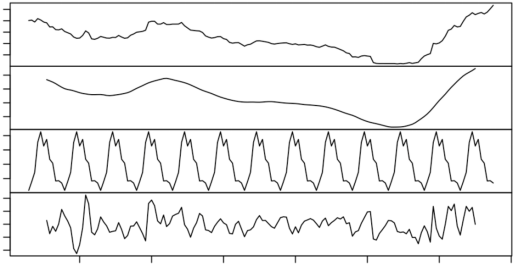
\includegraphics[width=0.8\textwidth]{picture/Decomposition4.png}};
            \node at (2.05,-0.3){\small 2012};
            \node at (3.85,-0.3){\small 2014};
            \node at (5.68,-0.3){\small 2016};
            \node at (7.48,-0.3){\small 2018};
            \node at (9.3,-0.3){\small 2020};
            \node at (11.15,-0.3){\small 2022};
            \node at (12.9,-0.3){\small 2024};
            \node at (6.4,-1){\textbf{Time}};

            \node at(-0.2,0.35)[rotate=90]{\small -0.4}; 
            \node at(-0.2,1.4)[rotate=90]{\small 0.2}; 
            \node at(-0.2,2.1)[rotate=90]{\small -0.05}; 
            \node at(-0.2,3.2)[rotate=90]{\small 0.10}; 
            \node at(-0.2,3.8)[rotate=90]{\small 1}; 
            \node at(-0.2,4.45)[rotate=90]{\small 3}; 
             \node at(-0.2,5.32)[rotate=90]{\small 1};
             \node at(-0.2,5.9)[rotate=90]{\small 3};
              \node at(-0.2,6.5)[rotate=90]{\small 5};
               \node at(-1,3.45)[rotate=90]{ \textbf{random seasonal trend observed}};
        \end{tikzpicture}
    \caption{Decomposition of additive time series}
   \label{De_n}
\end{figure}

Overall, the 2 year yield data after filling in the missing data and the 2 year swap data have similar trends and seasonality. 2 year yield data is also a non-stationary time series.

Therefore, we have sufficient evidence to believe that the 2 year yield data is reliable.




\subsubsection{The 1 year interbank rate}

For the absent data preceding August 2010, we leveraged the interbank rate for predictions. The method resembled our previous predictions. Given the continuous data absence in 2009 – a tumultuous year post the financial crisis – a straightforward linear regression based on the interbank rate was deemed unsuitable and the Random forests are still reliable.

\begin{figure}[H]
    \centering
        \begin{tikzpicture}[global scale = 1]
            \node[anchor=south west,inner sep=0] at (0,0) {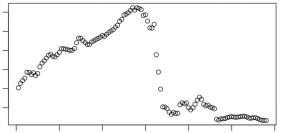
\includegraphics[width=0.3\textwidth]{picture/Interbank1.png}};
    \node at(0.3,-0.15){\small 0};
    \node at(1.075,-0.15){\small 20};
    \node at(1.85,-0.15){\small 40}; 
    \node at(2.625,-0.15){\small 60};
    \node at(3.4,-0.15){\small 80};
    \node at(4.175,-0.15){\small 100};
    \node at(4.95,-0.15){\small 120};   
    \node at(2.7,-0.8){\small month};
    \node at(2.63,2.8){{\textbf{\footnotesize Interbank Rate for 1 Year Period}}};

    \node at(-0.2,0.4)[rotate=90]{\small 4};    
       \node at(-0.2,0.76)[rotate=90]{\small 5}; 
    \node at(-0.2,1.1)[rotate=90]{\small 6};  
    \node at(-0.2,1.47)[rotate=90]{\small 7};
    \node at(-0.2,1.82)[rotate=90]{\small 8};  
    \node at(-0.2,2.2)[rotate=90]{\small 9};
    \node at(-1,1.2)[rotate=90]{\small Swap Rate in Percent};        

    
            \node[anchor=south west,inner sep=0] at (7,0) {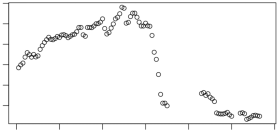
\includegraphics[width=0.3\textwidth]{picture/Yields5_2.png}};
            \node at(9.5,2.8){{\textbf{\footnotesize Yields Rate for 1 Year Period}}};

    \node at(7+0.3,-0.15){\small 0};
    \node at(7+1.075,-0.15){\small 20};
    \node at(7+1.85,-0.15){\small 40}; 
    \node at(7+2.625,-0.15){\small 60};
    \node at(7+3.4,-0.15){\small 80};
    \node at(7+4.175,-0.15){\small 100};
    \node at(7+4.95,-0.15){\small 120};   
    \node at(7+2.7,-0.8){\small month};



     \node at(7-0.2,0.2+0.32)[rotate=90]{\small 3};    
       \node at(7+-0.2,0.55+0.34)[rotate=90]{\small 4}; 
    \node at(7+-0.2,0.9+0.38)[rotate=90]{\small 5};  
    \node at(7+-0.2,1.25+0.39)[rotate=90]{\small 6};
    \node at(7+-0.2,1.6+0.43)[rotate=90]{\small 7};  
  \node at(7+-0.2,1.6+0.72)[rotate=90]{\small 8}; 

     \node at(6,1.2)[rotate=90]{\small Yields Rate in Percent};   
        \end{tikzpicture}
    \caption{}
    \label{Interbank1}
\end{figure}


After filled


\begin{figure}[H]
    \centering
        \begin{tikzpicture}[global scale = 1]
            \node[anchor=south west,inner sep=0] at (0,0) {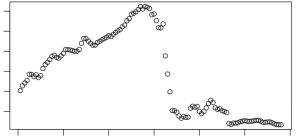
\includegraphics[width=0.3\textwidth]{picture/Interbank2.png}};
    \node at(0.3,-0.15){\small 0};
    \node at(1.075,-0.15){\small 20};
    \node at(1.85,-0.15){\small 40}; 
    \node at(2.625,-0.15){\small 60};
    \node at(3.4,-0.15){\small 80};
    \node at(4.175,-0.15){\small 100};
    \node at(4.95,-0.15){\small 120};   
    \node at(2.7,-0.8){\small month};
    \node at(2.63,2.8){{\textbf{\footnotesize Interbank Rate for 1 Year Period}}};

    \node at(-0.2,0.4)[rotate=90]{\small 4};    
       \node at(-0.2,0.76)[rotate=90]{\small 5}; 
    \node at(-0.2,1.1)[rotate=90]{\small 6};  
    \node at(-0.2,1.47)[rotate=90]{\small 7};
    \node at(-0.2,1.82)[rotate=90]{\small 8};  
    \node at(-0.2,2.2)[rotate=90]{\small 9};
    \node at(-1,1.2)[rotate=90]{\small swap rate in percent};        

    
            \node[anchor=south west,inner sep=0] at (7,0) {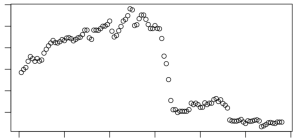
\includegraphics[width=0.3\textwidth]{picture/Yields6_2.png}};
            \node at(9.5,2.8){{\textbf{\footnotesize Yields Rate for 1 Year Period}}};

    \node at(7+0.3,-0.15){\small 0};
    \node at(7+1.075,-0.15){\small 20};
    \node at(7+1.85,-0.15){\small 40}; 
    \node at(7+2.625,-0.15){\small 60};
    \node at(7+3.4,-0.15){\small 80};
    \node at(7+4.175,-0.15){\small 100};
    \node at(7+4.95,-0.15){\small 120};   
    \node at(7+2.7,-0.8){\small Month};



     \node at(7-0.2,0.2+0.32)[rotate=90]{\small 3};    
       \node at(7+-0.2,0.55+0.34)[rotate=90]{\small 4}; 
    \node at(7+-0.2,0.9+0.38)[rotate=90]{\small 5};  
    \node at(7+-0.2,1.25+0.39)[rotate=90]{\small 6};
    \node at(7+-0.2,1.6+0.43)[rotate=90]{\small 7};  
  \node at(7+-0.2,1.6+0.72)[rotate=90]{\small 8}; 

     \node at(6,1.2)[rotate=90]{\small Yields Rate in Percent};   
        \end{tikzpicture}
    \caption{}
    \label{Interbank2}
\end{figure}



\begin{figure}[H]
    \centering
        \begin{tikzpicture}[global scale = 1]
            \node[anchor=south west,inner sep=0] at (0,0) {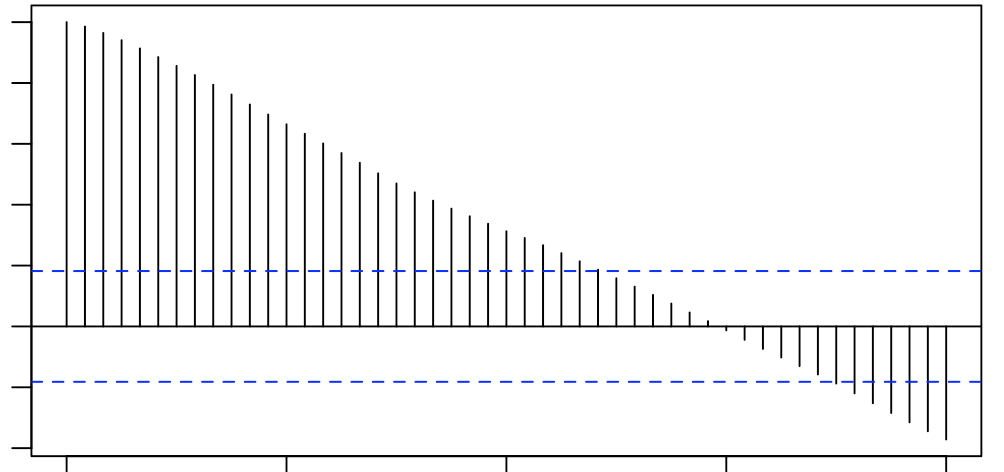
\includegraphics[width=0.3\textwidth]{picture/1.png}};
    \node at(0.35,-0.15){\small 0};
    \node at(1.43,-0.15){\small 1};     
    \node at(2.54,-0.15){\small 2};
    \node at(3.6,-0.15){\small 3};   
    \node at(4.68,-0.15){\small 4};
    \node at(2.63,-0.8){\small Lag};
    \node at(2.63,2.8){\textbf{\footnotesize Series Yield.ts1}};

    \node at(-0.2,0.2)[rotate=90]{\small -0.2};        
    \node at(-0.2,0.9)[rotate=90]{\small 0.2};  
    \node at(-0.2,1.6)[rotate=90]{\small 0.6};  
    \node at(-0.2,2.3)[rotate=90]{\small 1.0};  
    \node at(-1,1.2)[rotate=90]{\small ACF};        

    
            \node[anchor=south west,inner sep=0] at (7,0) {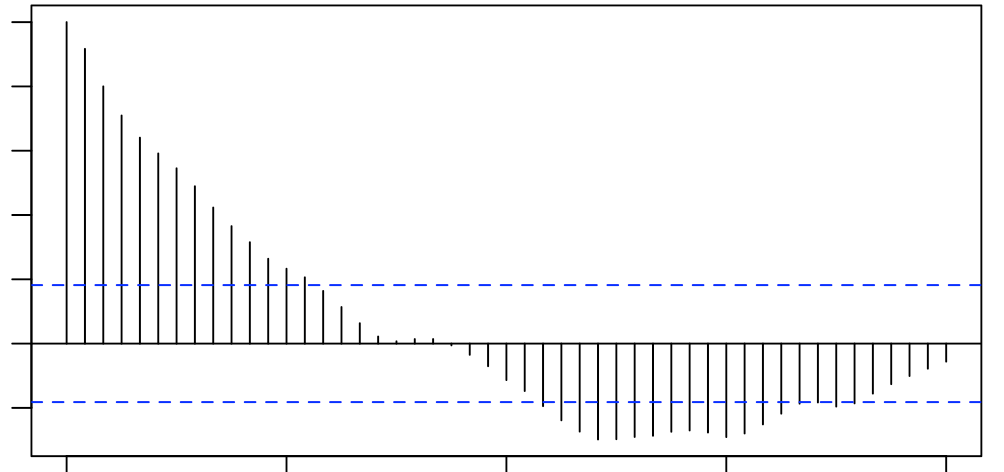
\includegraphics[width=0.3\textwidth]{picture/2.png}};
            \node at(9.5,2.8){\textbf{\footnotesize Series (Yield.ts1-mean(Yield.ts1))$^2$}};

    \node at(7+0.4,-0.15){\small 0.0};     
    \node at(7+1.4,-0.15){\small 0.5};
    \node at(7+2.55,-0.15){\small 1.0};   
    \node at(7+3.65,-0.15){\small 1.5};
    \node at(7+2.63,-0.8){\small Lag};

    \node at(7+-0.2,0.2)[rotate=90]{\small -0.0};        
    \node at(7+-0.2,0.9)[rotate=90]{\small 0.2};  
    \node at(7+-0.2,1.6)[rotate=90]{\small 0.6};  
    \node at(7+-0.2,2.3)[rotate=90]{\small 1.0};  
    \node at(7+-1,1.2)[rotate=90]{\small ACF};   
        \end{tikzpicture}
    \caption{}
    \label{Series15}
\end{figure}


% \begin{figure}[H]
%     \centering
%     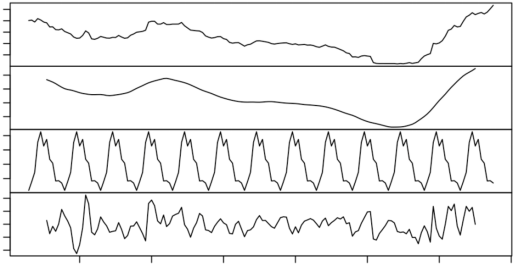
\includegraphics[width=0.8\textwidth]{picture/Decomposition4.png}
%   \vspace{20pt}\caption{\hyperref[Decomposition4]{Decomposition of Additive Time Series}}
%  %   \label{Decomposition}

%     \begin{picture}(0,0)
%         \put(0.365\textwidth,0.097\textwidth){\makebox(0,0)[lt]{\small{{2024}}}}
%         \put(0.25\textwidth,0.097\textwidth){\makebox(0,0)[lt]{\small{{2022}}}}
%         \put(0.145\textwidth,0.097\textwidth){\makebox(0,0)[lt]{\small{{2020}}}}
%         \put(0.03\textwidth,0.097\textwidth){\makebox(0,0)[lt]{\small{{2018}}}}
%         \put(-0.08\textwidth,0.097\textwidth){\makebox(0,0)[lt]{\small{{2016}}}}
%         \put(-0.19\textwidth,0.097\textwidth){\makebox(0,0)[lt]{\small{{2014}}}}
%         \put(-0.3\textwidth,0.097\textwidth){\makebox(0,0)[lt]{\small{{2012}}}}

%         \put(-0.43\textwidth,0.15\textwidth){\makebox(0,0)[lt]{\rotatebox{90}{\small{-0.4}}}}
%         \put(-0.43\textwidth,0.205\textwidth){\makebox(0,0)[lt]{\rotatebox{90}{\small{0.2}}}}
%         \put(-0.43\textwidth,0.25\textwidth){\makebox(0,0)[lt]{\rotatebox{90}{\small{-0.05}}}}
%         \put(-0.43\textwidth,0.33\textwidth){\makebox(0,0)[lt]{\rotatebox{90}{\small{0.10}}}}
%         \put(-0.43\textwidth,0.345\textwidth){\makebox(0,0)[lt]{\rotatebox{90}{\small{1}}}}
%         \put(-0.43\textwidth,0.39\textwidth){\makebox(0,0)[lt]{\rotatebox{90}{\small{3}}}}
%         \put(-0.43\textwidth,0.44\textwidth){\makebox(0,0)[lt]{\rotatebox{90}{\small{1}}}}
%         \put(-0.43\textwidth,0.47\textwidth){\makebox(0,0)[lt]{\rotatebox{90}{\small{3}}}}
%         \put(-0.43\textwidth,0.51\textwidth){\makebox(0,0)[lt]{\rotatebox{90}{\small{5}}}}

%         \put(-0.02\textwidth,0.07\textwidth){\makebox(0,0)[lt]{\textbf{Time}}}
%         \put(-0.47\textwidth,0.47\textwidth){\makebox(0,0)[lt]{\rotatebox{90}{\textbf{Random Seasonal Trend Observed}}}}

%     \end{picture}
% \end{figure}
\tikzset{global scale/.style={
    scale=#1,
    every node/.append style={scale=#1}
  }
}
\begin{figure}[H]
    \centering
        \begin{tikzpicture}[global scale = 1]
            \node[anchor=south west,inner sep=0] at (0,0) {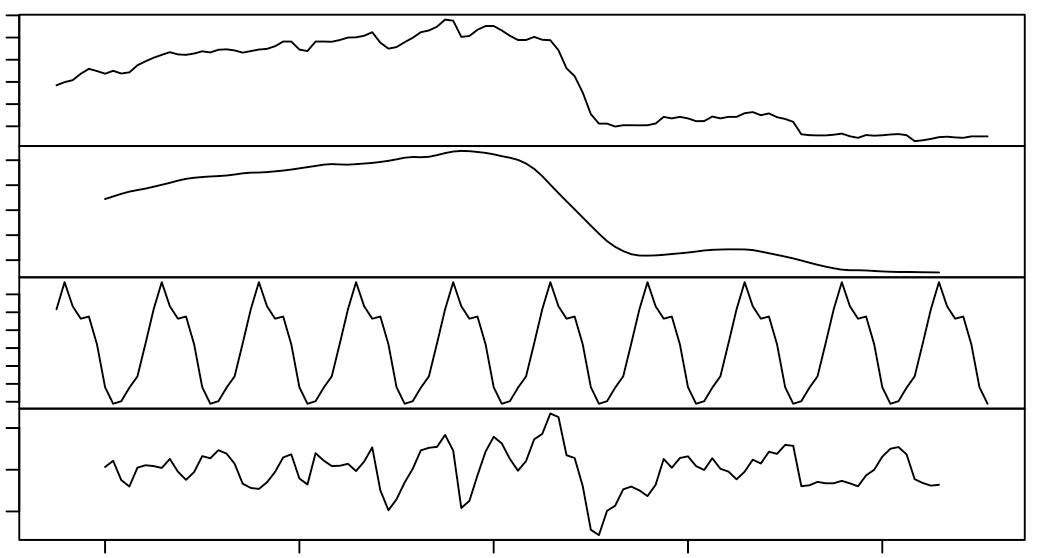
\includegraphics[width=0.8\textwidth]{picture/3.png}};
            \node at (2.05,-0.3){\small 2012};
            \node at (3.85,-0.3){\small 2014};
            \node at (5.68,-0.3){\small 2016};
            \node at (7.48,-0.3){\small 2018};
            \node at (9.3,-0.3){\small 2020};
            \node at (11.15,-0.3){\small 2022};
            \node at (12.9,-0.3){\small 2024};
            \node at (6.4,-1){\textbf{Time}};

            \node at(-0.2,0.35)[rotate=90]{\small -0.4}; 
            \node at(-0.2,1.4)[rotate=90]{\small 0.2}; 
            \node at(-0.2,2.1)[rotate=90]{\small -0.05}; 
            \node at(-0.2,3.2)[rotate=90]{\small 0.10}; 
            \node at(-0.2,3.8)[rotate=90]{\small 1}; 
            \node at(-0.2,4.45)[rotate=90]{\small 3}; 
             \node at(-0.2,5.32)[rotate=90]{\small 1};
             \node at(-0.2,5.9)[rotate=90]{\small 3};
              \node at(-0.2,6.5)[rotate=90]{\small 5};
               \node at(-1,3.45)[rotate=90]{ \textbf{random seasonal trend observed}};
        \end{tikzpicture}
    \caption{Decomposition of additive time series}
   \label{De4}
\end{figure}

Overall, the 1 year yield data after filling in the missing data and the 1 year interbank data have similar trends and seasonality. 1 year yield data is also a non-stationary time series.

Therefore, we have sufficient evidence to believe that the 1 year yield data is reliable.




\subsection{Final Data for 1 year and 2 year period yield}

\begin{figure}[H]
    \centering
        \begin{tikzpicture}[global scale = 1]
            \node[anchor=south west,inner sep=0] at (0,0) {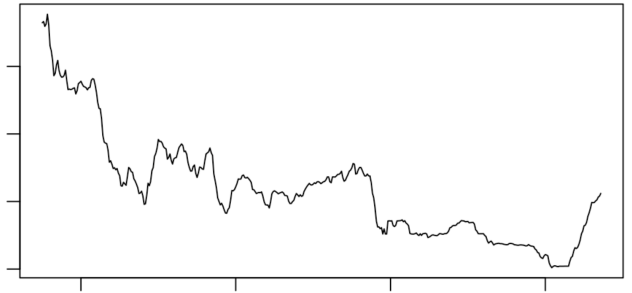
\includegraphics[width=0.8\textwidth]{picture/Yields7.png}};

    \node at(11.45,-0.3){\small 2020};  
    \node at(8.2,-0.3){\small 2010}; 
    \node at(4.95,-0.3){\small 2000}; 
    \node at(1.7,-0.3){\small 1990};    
    \node at(6.7,-1){\small Year};   


    \node at(-0.3,0.5)[rotate=90]{\small 0};    
    \node at(-0.3,1.93)[rotate=90]{\small 5};   
    \node at(-0.3,3.37)[rotate=90]{\small 10};    
    \node at(-0.3,4.75)[rotate=90]{\small 15};   

    \node at(-1,3)[rotate=90]{\small Yield Rate in Percent};   
    
        \end{tikzpicture}
    \caption{{Yields Rate for 1 Year Period}}
   \label{Yields19}
\end{figure}






\begin{figure}[H]
    \centering
        \begin{tikzpicture}[global scale = 1]
            \node[anchor=south west,inner sep=0] at (0,0) {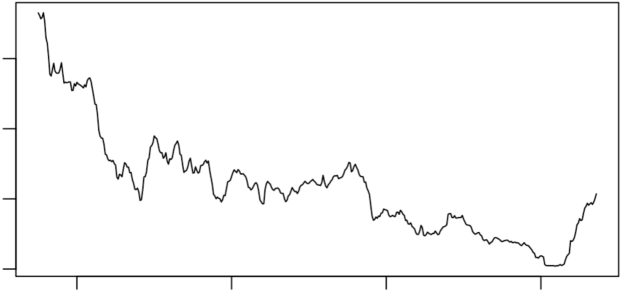
\includegraphics[width=0.8\textwidth]{picture/Yields8.png}};

    \node at(11.45,-0.3){\small 2020};  
    \node at(8.25,-0.3){\small 2010}; 
    \node at(4.95,-0.3){\small 2000}; 
    \node at(1.7,-0.3){\small 1990};    
    \node at(6.7,-1){\small Year};    


    \node at(-0.3,0.5)[rotate=90]{\small 0};    
    \node at(-0.3,2)[rotate=90]{\small 5};   
    \node at(-0.3,3.5)[rotate=90]{\small 10};    
    \node at(-0.3,4.9)[rotate=90]{\small 15};   

    \node at(-1,3)[rotate=90]{\small Yield rate in percent};   
    
        \end{tikzpicture}
    \caption{{Yields rate for 2 Year Period}}
    \label{Yields20}
\end{figure}

\subsection{Conversion of Daily Data to Monthly Data:}

Certain datasets, such as the US yield data, were provided on a daily basis. To standardize this with our monthly datasets, I utilized Pivot Tables and the average function to transform these daily figures into monthly averages.

\section{Economics Model}
The model used is similar to that used by Lloyd and Marin (2019)\footnote{as above \hyperref[lloyd2020exchange]{n1}} as the regression equations are the same, while the regression itself is run as a Newey-West regression. 

\begin{equation}
e_{j,t+k}\ -e_{j,t})\ =\ \beta_0+\beta_1(r_{j,t,k}\ -\ r_{i,t,k})\ +\ u_{i,t+k}
\end{equation}

In our first regression, looking at UIP and the conditions for it to hold true, we calculate the effects of the difference in nations continuously compounded returns, with the difference in exchange rates over a set of horizons, in our case 6 months, 12 months, 60 months and 120 months. In our model we are focussing on the United States and New Zealand, with the United States acting as our base country. This regression is used to examine whether UIP holds, as a coefficient of 1 would indicate that UIP does hold, as the exchange rate would then be determined such that returns would be similar between investing in either nation, either base or foreign. For this first regression no other variables were used as control variables, so the regression only included the dependent and explanatory variables. This regression is run as a Newey-West regression instead of a standard OLS due to the time series nature of the data, minimising the errors that may arise from autocorrelation or heteroskedasticity. In addition this brought another consideration, namely the optimal number lags. To determine this we utilised the rule laid out in \cite{lazarus2018har} to determine the truncation parameter, the rule being that the truncation parameter equals $1.3T^{1/3}$, with T representing the number of observations. Utilising this we were able to run a standard Newey-west regression to determine our output.

\begin{equation}
(e_{j,t+k}\ -e_{j,t})\ =\ \beta_0+\beta_1(r_{j,t,k}\ -\ r_{i,t,k})\ +\beta_1(S_{j,t}\ -S_{i,t})+\ u_{i,t+k}
\end{equation}

Similar methods were used in the second regression, a Newey-West with the truncation rule being similarly applied, except in this regression we introduced a new variable, the difference in yield curve slopes. Calculated by each nation's difference in the 3 month and 10 year yield, the difference in the results from each nation was added to the regression to expound it. In this case we analysed the slope variable as an explanatory variable that may affect the change in the exchange rate over time. All outputs were taken from a standard Newey-West regression, be it the coefficient results, or the adjusted R-squared’s calculated, with the only difference between regressions being the difference in horizons, and the inclusion of a new explanatory variable in a new regression.


\section{Model Analysis}


%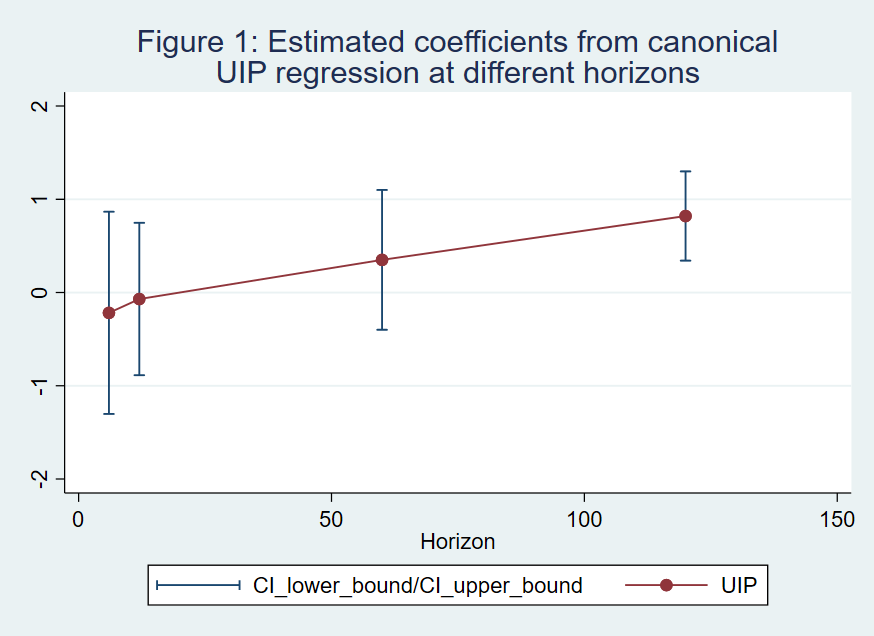
\includegraphics[scale=0.45]{picture/First_regression_graph.png}

\begin{figure}[H]
    \centering
        \begin{tikzpicture}[global scale = 1]
            \node[anchor=south west,inner sep=0] at (0,0) {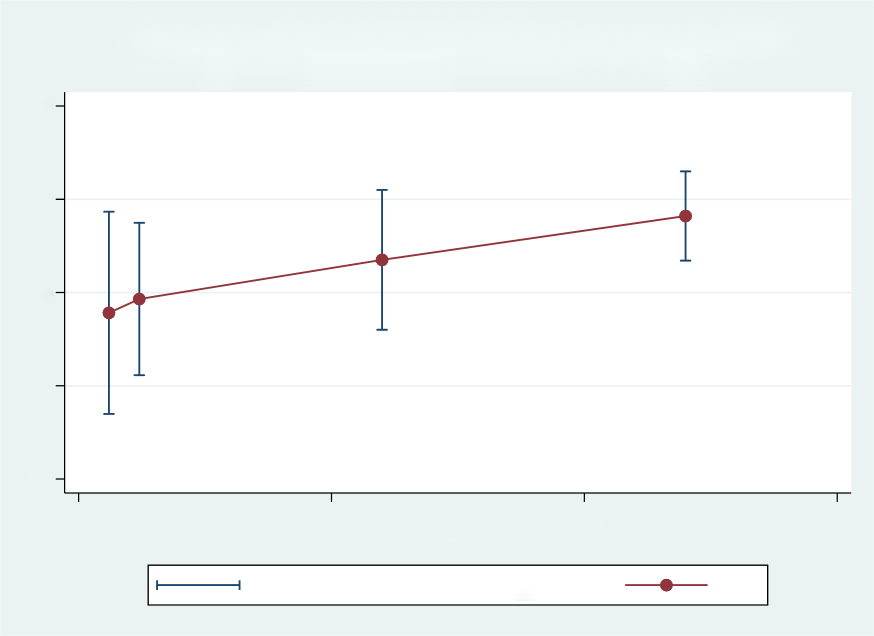
\includegraphics[width=0.8\textwidth]{picture/First_regression_graph_.png}};
        \node at(1.2,1.7){0};
        \node at(5.05,1.7){50};
        \node at(8.76,1.7){100};
        \node at(12.6,1.7){150};
        \node at(6.45,0.75){CI\_lower\_bound/CI\_upper\_bound};
        \node at(11.1,0.77){UIP};
        \node at(7,1.4){Horizon};

        \node at(0.5,2.25)[rotate=90]{-2};
        \node at(0.5,3.75)[rotate=90]{-1};
        \node at(0.5,5.2)[rotate=90]{0};
        \node at(0.5,6.6)[rotate=90]{1};
         \node at(0.5,8)[rotate=90]{2};
        
        \end{tikzpicture}
    \caption{Estimated coefficients from canonical UIP regression at different horizons}
    \label{E1}
\end{figure}

%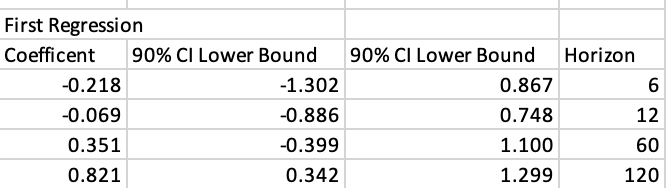
\includegraphics[scale=1]{picture/t1.png}

\begin{table}[H]
    \centering
    \caption{First Regression}
    \begin{tabular}{cccc}
    \hline
     Coefficent    &  90\% CI Lower Bound   &  90\% CI Lower Bound & Horizon  \\\hline
         -0.218   &  -1.302   & 0.867  &  6 \\
          -0.069      & -0.886    & 0.748  & 12  \\
                 0.351   &   -0.399  &  1.100 & 60  \\
               0.821   & 0.342    &  1.299 & 120  \\\hline
    \end{tabular}
    \label{t1}
\end{table}

The results of the first regression can be seen in figure 27 above and indicates similar results to those found in \cite{lloyd2020exchange}. The regressions shows that the null hypothesis for UIP set forward in section 2.1 of Lloyd and Marim (2020)\footnote{as above \hyperref[lloyd2020exchange]{n1}}, that $\beta_1 = 1$ for all k (horizon in our case) greater than 0, can not hold true for half of our horizons analysed. Looking at the individual coefficient outputs, we found that a 1 percentage point increase in the interest rate differential leads to a 0.218 depreciation in the USD for the 6 month horizon, a 0.691 depreciation for the 12 month horizon, a 0.351 appreciation for the 60 month horizon, and a 0.821 appreciation for the 120 month horizon. Further analysis shows that when looking at the outputs from this regression, we cannot establish statistical significance at the 10\% level for the coefficient for the regressions where the horizon variable is less than or equal to 60 months. In addition to this, for regressions with the length for 12 or 24 months, the 90\% confidence interval fails to overlap with the critical 1 value needed to fail to reject the null hypothesis established by the UIP, and as such it is rejected. This agrees with other empirical rejections noted in Lloyd and Marin (2020)\footnote{as above \hyperref[lloyd2020exchange]{n1}} establishing that the null hypothesis can be dismissed when the horizon analysed is small. The result gets more complex with the months set to 60, as we note a coefficient that is both not statistically significant, having a p-value of 0.441 and a 90\% confidence interval that overlaps with 0, but in addition has a confidence interval that overlap with the vital 1 value that would hold with UIP and the null hypothesis. As such this result can be viewed with scepticism, but we cannot reject the null hypothesis given the intervals overlapping with the 1 value (additional scepticism can be laid with a coefficient value of 0.35). The final regression, where the horizon is 120 months, does appear to result in a unique conclusion, in that in addition to a statistically significant coefficient (p-value = 0.005) the confidence interval also overlaps with the 1 value, in addition to a coefficient value that itself results in 0.82, the closest value to 1 from all regressions. This not only leads us to fail to reject the null hypothesis, indicating that UIP holds true, but in addition further enforces the statement referenced earlier, that for small values of time, the UIP will not hold. The evidence of the UIP holding (or stronger evidence that it does) as time increases indicates that the horizon used does alter the applicability of UIP. This can be seen in the data, as for all regressions, as the horizon increased, the coefficient increased $(-.218 < -0.691 < 0.351 < 0.821)$. The findings from regressions utilising only the singular variable to establish UIP indicate results reflective of those in Lloyd \& Narin, UIP holds only for values of t that are large.

\begin{figure}[H]
    \centering
        \begin{tikzpicture}[global scale = 1]
            \node[anchor=south west,inner sep=0] at (0,0) {\includegraphics[width=0.8\textwidth]{picture/Altered_regression_graph_.png}};
        \node at(1.2,1.7){0};
        \node at(5.05,1.7){50};
        \node at(8.9,1.7){100};
        \node at(12.6,1.7){150};
        \node at(6.45,0.75){CI\_lower\_bound/CI\_upper\_bound};
        \node at(11.1,0.77){Slope};
        \node at(7,1.4){Horizon};

        \node at(0.5,2.25)[rotate=90]{-10};
        \node at(0.5,4.18)[rotate=90]{-5};
        \node at(0.5,5.85)[rotate=90]{0};
        \node at(0.5,7.7)[rotate=90]{5};
    
        
        \end{tikzpicture}
    \caption{Estimated relative slope coefficients from augmented UIP regression}
    \label{E2}
\end{figure}


%\includegraphics[scale=1]{picture/t2.png}

\begin{table}[H]
    \centering
    \caption{Slope Regression}
    \begin{tabular}{cccc}
    \hline
     Coefficent    &  90\% CI Lower Bound   &  90\% CI Lower Bound & Horizon  \\\hline
         0.067   &  -2.638   & 2.773  &  6 \\
          1.167      & -2.696    & 5.030  & 12  \\
                 -2.151   &   -7.605  &  3.304 & 60  \\
                     1.375   & -3.223    &  5.972 & 120  \\\hline
    \end{tabular}
    \label{t2}
\end{table}

The results from the second regression (seen above Figure 28) indicate different findings as to the impact of the slope variable as an explanatory variable. Firstly, the results from the regression indicate that a 1 percentage point increase in the slope differential leads to a 0.067 appreciation in the USD for the 6 month horizon, a 1.167 appreciation for the 12 month horizon, a -2.151 depreciation for the 60 month horizon, and a 1.375 appreciation for the 120 month horizon.The first aspect of note is the large confidence intervals that come with all values. Every one of the regressions results in an overlapping of the slope coefficient’s confidence interval with 0, indicating a lack of statistical significance. This finding is enhanced by the p-values, all of which sit above 0.516. This puts into question the importance of the slope variable in determining the different horizon exchange rate dynamic.  Further analysis of the results indicate that the relationship is not linear, as while the coefficient increases from 12 months to 24 months, it decreases to the smallest value at 60 months before increasing again to the highest value from the 120 month horizon. This shape also works as an almost perfect inverse of the shape found in Lloyd and Marin (2020)\footnote{as above \hyperref[lloyd2020exchange]{n1}}, as their tent shape is found in reverse in figure 2. Another aspect is worth noting, and that is that none of the coefficients are statistically different from any other. The confidence intervals for all coefficients overlap with all other variable coefficients. Analysing what the coefficients tell us about the empirical impact of the slope variable, one interpretation of the slope variable could be as a risk indicator, as noted in the introduction of Lloyd and Marin (2020)\footnote{as above \hyperref[lloyd2020exchange]{n1}}. This can be worked to analyse our findings. In this case any coefficients of a significant value or pattern would indicate that business cycle risk both has an effect on exchange rates and in addition is reflected by the relative yield curve slope. If we assume that the reflective property holds we can see that the risk mentioned does not appear to have a significant effect on the exchange rate in this data given the lack of statistical significance for any horizon. This again works against the findings in Lloyd and Marin (2020)\footnote{as above \hyperref[lloyd2020exchange]{n1}}, as their establishment of the slope coefficient significance and the implication of risk inside the model is not substantiated in our findings. Their assertion that the slope differential between nations works largest in any given timeframe also does not hold, as all are seen with the same insignificance and none are statistically different from any other. Overall the results from these regressions indicate that the slope variable may not be of large importance to the exchange rate measured here, and the risk it may reflect also appears absent in influencing the exchange rate.

\begin{figure}[H]
    \centering
        \begin{tikzpicture}[global scale = 1]
            \node[anchor=south west,inner sep=0] at (0,0) {\includegraphics[width=0.8\textwidth]{picture/Adjusted-R2_.png}};
        \node at(1.2,1.7){0};
        \node at(5.05,1.7){50};
        \node at(8.9,1.7){100};
        \node at(12.6,1.7){150};
        \node at(4.8,0.75){adjusted\_r2};
        \node at(9.5,0.75){adjusted\_r2\_with\_Slope};
        \node at(7,1.4){Horizon};

        \node at(0.5,2.36)[rotate=90]{0};
        \node at(0.5,3.85)[rotate=90]{.05};
        \node at(0.5,5.4)[rotate=90]{.1};
        \node at(0.5,6.5)[rotate=90]{.15};
        \node at(0.5,7.85)[rotate=90]{.2};
        \node at(-0.5,5)[rotate=90]{Adjusted-R-squared};
        
        \end{tikzpicture}
    \caption{Explantary power of UIP regression augmented with relative yield curve slope at different horizons}
    \label{E3}
\end{figure}


%\includegraphics[scale=1]{picture/t3.png}
\begin{table}[H]
    \centering
    \caption{Adjusted R-Squares}
    \begin{tabular}{ccc}
    \hline
     First Regression    & Slope Regression   &  Horizon   \\\hline
         -0.0009  & -0.0032  &  6 \\
          -0.0021      & 0.0001    &  12  \\
                 0.0080   &   0.0155 & 60  \\
               0.1659   & 0.1688 & 120  \\\hline 
    \end{tabular}
    \label{t3}
\end{table}

The final lot of results (shown above Figure 30) found revolves around the adjusted r-squareds found from each of the regressions, both those with the slope and without. What was found is intuitive from the findings discussed previously, notable that the larger the horizon the larger the adjusted r-squared, from extremely minor negative values (-0.001 and -0.003) with the smallest horizon the values of 0.17 (rounded) with a 120 month horizon for both regressions. This further goes to reinforce the idea that was referenced early on, UIP does not hold for smaller horizons, as looking at the adjusted R-squared (particularly for the first regression) it becomes clear that the coefficient utilised to examine UIP holds more importance in the regression as the horizon increases. Another aspect worth investigating is the difference between the two adjusted R-squared flows between the two different loads of regressions, those with and those without the slope variable. While the smaller horizon shows the simpler regression having a slightly higher adjusted R-squared than the more complex regression, the relationship flips for all other horizons, and is larger for two of those three horizons. This would indicate that the addition of the slope variable is beneficial to the regression, indicating that the relative slope of yield curves acts as an additional component of ERRP (exchange rate risk premia).

\section{Conclusion}
Based on the empirical exercises from our report, we identified how UIP fails to hold for short horizons, collaborating with the findings discovered in the \cite{lloyd2020exchange} paper that our work is based on. This is supplemented by the evidence showing more support for the UIP condition as the horizon increases, demonstrating that the UIP condition between the US and New Zealand behaves similarly to those researched beyond this paper in how its applicability differs over varying horizons. In addition we identified the differences in yield curve slopes as a possible additional variable in analysing the exchange rate fluctuations over time and its benefit to the overall regression run. Our findings differ from Lloyd and Marin\footnote{as above \hyperref[lloyd2020exchange]{n1}} here with the yield curves relative impact on exchange rate fluctuations in themselves, as our empirical findings worked to indicate that the risk that may be displayed in this variable was not significant in the determination of exchange rate fluctuations. This finding is additionally interesting when compared to later findings indicating the variables benefit to the overall regression run. Our findings suggest that common outside findings, such as the exclusively long term presence of UIP, hold, while other conclusions may not be applicable to the exchange rate we analysed. The results of this detail how the consideration of the UIP condition by actors such as governments or investors may be dismissed in short term horizons while the impact of decisions such as monetary policy should be considered by its possible effect on the longer term exchange rate fluctuations. It should be noted that our findings are limited, as UIP is only analysed with a singular variable in the regression model, and further analysis including that of the yield slope was additionally only done with a bare bones regression analysis, including only the regressor from the previous regression as another variable in the regression. Based on this there may be concerns around omitted variable bias. In addition, while our analysis was performed with the latest formations of the truncation parameter, it may be beneficial to perform similar analysis with varying models before definitive conclusions are drawn. In addition the data used comes with limitations, primarily the discontinuities within the one-year yield rate data could introduce omitted variable biases, potentially skewing the outcomes of our linear regression. Our heavy reliance on the ADF test, though academically sound, could pose risks, given that singular dependence might overlook subtleties in complex datasets. Additionally, the use of simple linear regression in the face of such data gaps might be less than ideal, possibly leading to misleading results. Furthermore, to find the missing variables, we only use swap rate and interbank rate to predict yield rate. This may be inaccurate, if we use more variables and more models for prediction, this will have closer to the actual data. Furthermore, ask RBNZ to get a not missing variable data will be also improve the model accuracy. It is also apply to the daily data. Overall our findings are both supportive and distinct from the paper that our research was based on, implying the existence of different conditions in the exchange rate fluctuations between the United States and New Zealand from those studied in \cite{lloyd2020exchange}.










\printbibliography

\newpage

\pagenumbering{arabic}
\appendix

\section{Appendix A - Figure}
\begin{lstlisting}[language=R]

\end{lstlisting}


\setcounter{figure}{0}
\begin{figure}[H]
    \centering
        \begin{tikzpicture}[global scale = 1.1]
            \node[anchor=south west,inner sep=0] at (0,0) {\includegraphics[width=0.8\textwidth]{picture/Decomposition.png}};
            \node at (2.1,-0.3){\small 2012};
            \node at (3.9,-0.3){\small 2014};
            \node at (5.7,-0.3){\small 2016};
            \node at (7.6,-0.3){\small 2018};
            \node at (9.5,-0.3){\small 2020};
            \node at (11.4,-0.3){\small 2022};
            \node at (13.2,-0.3){\small 2024};
            \node at (6.4,-1){\textbf{Time}};

            \node at(-0.2,0.35)[rotate=90]{\small -0.3}; 
            \node at(-0.2,1.25)[rotate=90]{\small 0.1}; 
            \node at(-0.2,1.8)[rotate=90]{\small -0.06}; 
            \node at(-0.2,2.9)[rotate=90]{\small 0.02}; 
            \node at(-0.2,3.75)[rotate=90]{\small 1}; 
            \node at(-0.2,4.35)[rotate=90]{\small 3}; 
            \node at(-0.2,4.95)[rotate=90]{\small 5};
             \node at(-0.2,5.1)[rotate=90]{\small 0};
             \node at(-0.2,5.62)[rotate=90]{\small 2};
              \node at(-0.2,6.15)[rotate=90]{\small 4};
               \node at(-0.2,6.75)[rotate=90]{\small 6};
               \node at(-1,3.5)[rotate=90]{ \textbf{random seasonal trend observed}};
        \end{tikzpicture}
    \caption{\hyperref[Decomposition1]{\textcolor{black}{Decomposition of additive time series}}}
 %   \label{Series1}
\end{figure}



\begin{figure}[H]
    \centering
        \begin{tikzpicture}[global scale = 2.5]
            \node[anchor=south west,inner sep=0] at (0,0) {\includegraphics[width=0.3\textwidth]{picture/Series1.png}};
    \node at(0.35,-0.15){\small 0};
    \node at(1.42,-0.15){\small 1};     
    \node at(2.56,-0.15){\small 2};
    \node at(3.67,-0.15){\small 3};   
    \node at(4.78,-0.15){\small 4};
    \node at(2.63,-0.8){\small Lag};
    \node at(2.63,2.8){{\textbf{\footnotesize Series swap.ts}}};

    \node at(-0.2,0.2)[rotate=90]{\small -0.2};        
    \node at(-0.2,0.9)[rotate=90]{\small 0.2};  
    \node at(-0.2,1.6)[rotate=90]{\small 0.6};  
    \node at(-0.2,2.3)[rotate=90]{\small 1.0};  
    \node at(-1,1.2)[rotate=90]{\small ACF};        
        \end{tikzpicture}
    \caption{\hyperref[Series1]{{\textcolor{black}{Series swap.ts}}}}
  %  \label{Series1}
\end{figure}

% \setcounter{figure}{1}
    
\addtocounter{figure}{-1}   

 \begin{figure}[H]
    \centering
        \begin{tikzpicture}[global scale = 2.5]   
            \node[anchor=south west,inner sep=0] at (7,0) {\includegraphics[width=0.3\textwidth]{picture/Series2.png}};
            \node at(9.5,2.8){ \textbf{\footnotesize Series (swap.ts-mean(swap.ts))$^2$}};
     \node at(7+0.35,-0.15){\small 0};
    \node at(7+1.42,-0.15){\small 1};     
    \node at(7+2.56,-0.15){\small 2};
    \node at(7+3.67,-0.15){\small 3};   
    \node at(7+4.78,-0.15){\small 4};
    \node at(7+2.63,-0.8){\small Lag};

    \node at(7+-0.2,0.2)[rotate=90]{\small -0.2};        
    \node at(7+-0.2,0.9)[rotate=90]{\small 0.2};  
    \node at(7+-0.2,1.6)[rotate=90]{\small 0.6};  
    \node at(7+-0.2,2.3)[rotate=90]{\small 1.0};  
    \node at(7+-1,1.2)[rotate=90]{\small ACF};   
        \end{tikzpicture}
    \caption{\hyperref[Series1]{{\textcolor{black}{Series (swap.ts-mean(swap.ts))$^2$}}}}
   % \label{Series2}
\end{figure}



\begin{figure}[H]
    \centering
        \begin{tikzpicture}[global scale = 1.1]
            \node[anchor=south west,inner sep=0] at (0,0) {\includegraphics[width=0.8\textwidth]{picture/Swap.png}};
    \node at(12.95,-0.3){\small 2024};
    \node at(11.1,-0.3){\small 2022};     
    \node at(9.4,-0.3){\small 2020}; 
    \node at(7.5,-0.3){\small 2018}; 
    \node at(5.7,-0.3){\small 2016}; 
    \node at(3.9,-0.3){\small 2014}; 
    \node at(2.2,-0.3){\small 2012};      
    \node at(6.7,-1){\small Month};   


    

    \node at(-0.3,0.5)[rotate=90]{\small 0};    
    \node at(-0.3,1.5)[rotate=90]{\small 1};   
    \node at(-0.3,2.5)[rotate=90]{\small 2};    
    \node at(-0.3,3.5)[rotate=90]{\small 3};   
    \node at(-0.3,4.5)[rotate=90]{\small 4};    
    \node at(-0.3,5.5)[rotate=90]{\small 5};   
    \node at(-1,3)[rotate=90]{\small Swap Rate in Percent};   
    
        \end{tikzpicture}
     \caption{\hyperref[Swap]{\textcolor{black}{Swap Rate for 2 Year Period}}}
  %  \label{Swap}
\end{figure}





\begin{figure}[H]
    \centering
        \begin{tikzpicture}[global scale = 2.5]
            \node[anchor=south west,inner sep=0] at (0,0) {\includegraphics[width=0.3\textwidth]{picture/Series2_1.png}};
   \node at(0.35,-0.15){\small 0};
    \node at(1.46,-0.15){\small 1};     
    \node at(2.55,-0.15){\small 2};
    \node at(3.65,-0.15){\small 3};   
    \node at(4.75,-0.15){\small 4};
    \node at(2.63,-0.8){\small Lag};
    \node at(2.63,2.8){\textbf{\footnotesize{Series swap.ts1}}};

    \node at(-0.2,0.2)[rotate=90]{\small -0.2};        
    \node at(-0.2,0.9)[rotate=90]{\small 0.2};  
    \node at(-0.2,1.6)[rotate=90]{\small 0.6};  
    \node at(-0.2,2.3)[rotate=90]{\small 1.0};  
    \node at(-1,1.2)[rotate=90]{\small ACF};        
        \end{tikzpicture}
    \caption{\hyperref[Series21]{{\textcolor{black}{Series swap.ts1}}}}
  %  \label{Series21}
\end{figure}

\addtocounter{figure}{-1}  

\begin{figure}[H]
    \centering
        \begin{tikzpicture}[global scale = 2.5]    
            \node[anchor=south west,inner sep=0] at (7,0) {\includegraphics[width=0.3\textwidth]{picture/Series2_2.png}};
            \node at(9.5,2.8){\textbf{\fontsize{6pt}{6pt}\selectfont Series (swap.ts1-mean(swap.ts1))$^2$}};

    \node at(7+0.4,-0.15){\small 0.0};     
    \node at(7+1.6,-0.15){\small 0.5};
    \node at(7+2.8,-0.15){\small 1.0};   
    \node at(7+4.1,-0.15){\small 1.5};
    \node at(7+2.63,-0.8){\small Lag};

    \node at(7+-0.2,0.2)[rotate=90]{\small -0.0};        
    \node at(7+-0.2,0.9)[rotate=90]{\small 0.2};  
    \node at(7+-0.2,1.6)[rotate=90]{\small 0.6};  
    \node at(7+-0.2,2.3)[rotate=90]{\small 1.0};  
    \node at(7+-1,1.2)[rotate=90]{\small ACF};   
        \end{tikzpicture}
    \caption{\hyperref[Series21]{{\textcolor{black}{Series (swap.ts1-mean(swap.ts1))$^2$}}}}
  %  \label{Series22}
\end{figure}


\tikzset{global scale/.style={
    scale=#1,
    every node/.append style={scale=#1}
  }
}
\begin{figure}[H]
    \centering
        \begin{tikzpicture}[global scale = 1.1]
            \node[anchor=south west,inner sep=0] at (0,0) {\includegraphics[width=0.8\textwidth]{picture/Decomposition2.png}};
            \node at (2.1,-0.3){\small 2012};
            \node at (3.9,-0.3){\small 2014};
            \node at (5.7,-0.3){\small 2016};
            \node at (7.5,-0.3){\small 2018};
            \node at (9.35,-0.3){\small 2020};
            \node at (11.3,-0.3){\small 2022};
            \node at (13.2,-0.3){\small 2024};
            \node at (6.4,-1){\textbf{\footnotesize Time}};

            \node at(-0.2,0.6)[rotate=90]{\small -0.2}; 
            \node at(-0.2,1.4)[rotate=90]{\small 0.2}; 
            \node at(-0.2,2)[rotate=90]{\small -0.06}; 
            \node at(-0.2,2.95)[rotate=90]{\small 0.02}; 
            \node at(-0.2,3.78)[rotate=90]{\small 1}; 
            \node at(-0.2,4.4)[rotate=90]{\small 3}; 
            \node at(-0.2,5)[rotate=90]{\small 5};
             \node at(-0.2,5.15)[rotate=90]{\small 0};
             \node at(-0.2,5.65)[rotate=90]{\small 2};
              \node at(-0.2,6.22)[rotate=90]{\small 4};
           \node at(-1,3.5)[rotate=90]{\textbf{\footnotesize Random Seasonal Trend Observed}};
        \end{tikzpicture}
    \caption{\hyperref[D2]{\textcolor{black}{Decomposition of additive time series}}}
 %   \label{Series1}
\end{figure}




\begin{figure}[H]
    \centering
        \begin{tikzpicture}[global scale = 1.1]
            \node[anchor=south west,inner sep=0] at (0,0) {\includegraphics[width=0.8\textwidth]{picture/in_.png}};
    \node at(11.3,-0.3){\small 2012};     
    \node at(8.9,-0.3){\small 2010}; 
    \node at(6.4,-0.3){\small 2008}; 
    \node at(4,-0.3){\small 2006}; 
    \node at(1.5,-0.3){\small 2004}; 
    \node at(6.4,-1){\small month};   
 
    \node at(-0.3,1.5)[rotate=90]{\small 4};   
    \node at(-0.3,2.6)[rotate=90]{\small 5};    
    \node at(-0.3,3.8)[rotate=90]{\small 6};   
    \node at(-0.3,4.9)[rotate=90]{\small 7};    
    \node at(-0.3,6)[rotate=90]{\small 8};  
    \node at(-0.3,7.3)[rotate=90]{\small 9}; 
    \node at(-1,4)[rotate=90]{\small Interbank Rate in Percent};   
    
        \end{tikzpicture}
    \caption{\hyperref[Interbankrate]{\textcolor{black}{Interbank Rate for 1 Year Period}}}
    
\end{figure}


\begin{figure}[H]
    \centering
        \begin{tikzpicture}[global scale = 2.5]
            \node[anchor=south west,inner sep=0] at (0,0) {\includegraphics[width=0.3\textwidth]{picture/in1_.png}};
    \node at(0.35,-0.15){\small 0};
    \node at(1.423,-0.15){\small 1};     
    \node at(2.52,-0.15){\small 2};
    \node at(3.603,-0.15){\small 3};   
    \node at(4.7,-0.15){\small 4};
    \node at(2.63,-0.8){\small Lag};
    \node at(2.63,3.5){\small \textbf{\footnotesize Series Interbank.ts}};

    \node at(-0.2,0.3)[rotate=90]{\small -0.4};        
    \node at(-0.2,1.05)[rotate=90]{\small 0.0};  
    \node at(-0.2,1.8)[rotate=90]{\small 0.4};  
    \node at(-0.2,2.5)[rotate=90]{\small 0.8};  
    \node at(-1,1.2)[rotate=90]{\small ACF};        
        \end{tikzpicture}
    \caption{\hyperref[I7]{\textcolor{black}{Series Interbank.ts}}}
   %\label{I7}
\end{figure}
\addtocounter{figure}{-1}  
 
\begin{figure}[H]
    \centering
        \begin{tikzpicture}[global scale = 2.5]   
            \node[anchor=south west,inner sep=0] at (7,0) {\includegraphics[width=0.3\textwidth]{picture/in2_.png}};
            \node at(9.5,3.5){\small \textbf{\fontsize{4pt}{3pt}\selectfont  Series (Interbank.ts-mean(Interbank.ts))$^2$}};

    \node at(7.05+0.35,-0.15){\small 0};
    \node at(7.05+1.423,-0.15){\small 1};     
    \node at(7.05+2.52,-0.15){\small 2};
    \node at(7.05+3.603,-0.15){\small 3};   
    \node at(7.05+4.7,-0.15){\small 4};
    \node at(7.05+2.63,-0.8){\small Lag};

    \node at(7+-0.2,0.4)[rotate=90]{\small -0.2};        
    \node at(7+-0.2,1.2)[rotate=90]{\small 0.2};  
    \node at(7+-0.2,2)[rotate=90]{\small 0.6};  
    \node at(7+-0.2,2.7)[rotate=90]{\small 1.0};  
    \node at(7+-1,1.2)[rotate=90]{\small ACF};   
        \end{tikzpicture}
    \caption{\hyperref[I7]{\textcolor{black}{Series (Interbank.ts-mean(Interbank.ts))$^2$}}}
   %\label{I7}
\end{figure}


\begin{figure}[H]
    \centering
        \begin{tikzpicture}[global scale = 1.1]
            \node[anchor=south west,inner sep=0] at (0,0) {\includegraphics[width=0.8\textwidth]{picture/in3_.png}};
            \node at (1.45,-0.3){\small 2004};
            \node at (3.9,-0.3){\small 2006};
            \node at (6.3,-0.3){\small 2008};
            \node at (8.8,-0.3){\small 2010};
            \node at (11.2,-0.3){\small 2012};

            \node at (6.4,-1){\textbf{\footnotesize Time}};

            \node at(-0.2,0.42)[rotate=90]{\small -1.0}; 
            \node at(-0.2,1.2)[rotate=90]{\small 0.0}; 
            \node at(-0.2,2)[rotate=90]{\small 1.0}; 
            \node at(-0.2,2.7)[rotate=90]{\small -0.1}; 
            \node at(-0.2,3.5)[rotate=90]{\small 0.1}; 
            \node at(-0.2,4.55)[rotate=90]{\small 4}; 
            \node at(-0.2,5.2)[rotate=90]{\small 6};
            \node at(-0.2,5.85)[rotate=90]{\small 8};
             \node at(-0.2,6.55)[rotate=90]{\small 4};
             \node at(-0.2,7.2)[rotate=90]{\small 6};
              \node at(-0.2,7.845)[rotate=90]{\small 8};
           \node at(-1,4)[rotate=90]{\textbf{\footnotesize Random Seasonal Trend Observed}};
        \end{tikzpicture}
    \caption{\hyperref[in3]{\textcolor{black}{Decomposition of additive time series}}}
 %   \label{Series1}
\end{figure}


% \begin{figure}[H]
%     \centering
%     \includegraphics[width=0.8\textwidth]{picture/Decomposition2.png}
%   \vspace{20pt}\caption{Decomposition of Additive Time Series}
%     \label{Decomposition2}

%     \begin{picture}(0,0)
%         \put(0.37\textwidth,0.097\textwidth){\makebox(0,0)[lt]{\small{{2024}}}}
%         \put(0.26\textwidth,0.097\textwidth){\makebox(0,0)[lt]{\small{{2022}}}}
%         \put(0.15\textwidth,0.097\textwidth){\makebox(0,0)[lt]{\small{{2020}}}}
%         \put(0.04\textwidth,0.097\textwidth){\makebox(0,0)[lt]{\small{{2018}}}}
%         \put(-0.075\textwidth,0.097\textwidth){\makebox(0,0)[lt]{\small{{2016}}}}
%         \put(-0.19\textwidth,0.097\textwidth){\makebox(0,0)[lt]{\small{{2014}}}}
%         \put(-0.3\textwidth,0.097\textwidth){\makebox(0,0)[lt]{\small{{2012}}}}

%         \put(-0.43\textwidth,0.16\textwidth){\makebox(0,0)[lt]{\rotatebox{90}{\small{-0.2}}}}
%         \put(-0.43\textwidth,0.205\textwidth){\makebox(0,0)[lt]{\rotatebox{90}{\small{0.2}}}}
%         \put(-0.43\textwidth,0.25\textwidth){\makebox(0,0)[lt]{\rotatebox{90}{\small{-0.06}}}}
%         \put(-0.43\textwidth,0.306\textwidth){\makebox(0,0)[lt]{\rotatebox{90}{\small{0.02}}}}
%         \put(-0.43\textwidth,0.348\textwidth){\makebox(0,0)[lt]{\rotatebox{90}{\small{1}}}}
%         \put(-0.43\textwidth,0.383\textwidth){\makebox(0,0)[lt]{\rotatebox{90}{\small{3}}}}
%         \put(-0.43\textwidth,0.425\textwidth){\makebox(0,0)[lt]{\rotatebox{90}{\small{50}}}}
%         \put(-0.43\textwidth,0.46\textwidth){\makebox(0,0)[lt]{\rotatebox{90}{\small{2}}}}
%         \put(-0.43\textwidth,0.49\textwidth){\makebox(0,0)[lt]{\rotatebox{90}{\small{4}}}}

%         \put(-0.02\textwidth,0.07\textwidth){\makebox(0,0)[lt]{\textbf{Time}}}
%         \put(-0.47\textwidth,0.47\textwidth){\makebox(0,0)[lt]{\rotatebox{90}{\textbf{random seasonal trend observed}}}}

%     \end{picture}
% \end{figure}





\begin{figure}[H]
    \centering
        \begin{tikzpicture}[global scale = 2.5]
            \node[anchor=south west,inner sep=0] at (0,0) {\includegraphics[width=0.3\textwidth]{picture/Swap2_1.png}};
    \node at(0.35,-0.15){\small 0};
    \node at(1.74,-0.15){\small 50};     
    \node at(3.2,-0.15){\small 100};
    \node at(4.65,-0.15){\small 150};   
    \node at(2.7,-0.8){\small Month};
    \node at(2.63,2.8){\textbf{\footnotesize {Swap Rate for 1 Year Period}}};

    \node at(-0.2,0.2)[rotate=90]{\small 0};    
       \node at(-0.2,0.55)[rotate=90]{\small 1}; 
    \node at(-0.2,0.9)[rotate=90]{\small 2};  
    \node at(-0.2,1.25)[rotate=90]{\small 3};
    \node at(-0.2,1.6)[rotate=90]{\small 4};  
    \node at(-0.2,1.95)[rotate=90]{\small 5};
    \node at(-0.2,2.3)[rotate=90]{\small 6};  
    \node at(-1,1.2)[rotate=90]{\small Swap Rate in Percent};        
        \end{tikzpicture}
    \caption{\hyperref[Swap21]{{\textcolor{black}{Swap Rate for 1 Year Period}}}}
   % \label{Swap21}
\end{figure}
\addtocounter{figure}{-1}  
\begin{figure}[H]
    \centering
        \begin{tikzpicture}[global scale = 2.5]    
            \node[anchor=south west,inner sep=0] at (7,0) {\includegraphics[width=0.3\textwidth]{picture/Yields.png}};
            \node at(9.5,2.8){\textbf{\footnotesize Yields Rate for 1 Year Period}};

    \node at(7+0.35,-0.15){\small 0};
    \node at(7+1.74,-0.15){\small 50};     
    \node at(7+3.2,-0.15){\small 100};
    \node at(7+4.65,-0.15){\small 150};   
    \node at(7+2.7,-0.8){\small month};


     \node at(7-0.2,0.2)[rotate=90]{\small 0};    
       \node at(7+-0.2,0.55)[rotate=90]{\small 1}; 
    \node at(7+-0.2,0.9)[rotate=90]{\small 2};  
    \node at(7+-0.2,1.25)[rotate=90]{\small 3};
    \node at(7+-0.2,1.6)[rotate=90]{\small 4};  
    \node at(7+-0.2,1.95)[rotate=90]{\small 5};

     \node at(6,1.2)[rotate=90]{\small yields rate in percent};   
        \end{tikzpicture}
    \caption{\hyperref[Swap21]{\textcolor{black}{Yields Rate for 1 Year Period}}}
   % \label{Yields2}
\end{figure}



\begin{figure}[H]
    \centering
        \begin{tikzpicture}[global scale = 2.5]
            \node[anchor=south west,inner sep=0] at (0,0) {\includegraphics[width=0.3\textwidth]{picture/Swap3_1.png}};
    \node at(0.35,-0.15){\small 0};
    \node at(1.74,-0.15){\small 50};     
    \node at(3.2,-0.15){\small 100};
    \node at(4.65,-0.15){\small 150};   
    \node at(2.7,-0.8){\small month};
    \node at(2.63,2.8){ \textbf{\footnotesize Swap Rate for 2 Year Period}};

    \node at(-0.2,0.2)[rotate=90]{\small 0};    
       \node at(-0.2,0.6)[rotate=90]{\small 1}; 
    \node at(-0.2,0.95)[rotate=90]{\small 2};  
    \node at(-0.2,1.35)[rotate=90]{\small 3};
    \node at(-0.2,1.72)[rotate=90]{\small 4};  
    \node at(-0.2,2.1)[rotate=90]{\small 5};
    \node at(-1,1.2)[rotate=90]{\small swap rate in percent};        
        \end{tikzpicture}
    \caption{\hyperref[Swap31]{\textcolor{black}{Swap Rate for 2 Year Period}}}
    \label{Swap31}
\end{figure}
    \addtocounter{figure}{-1}  
 
\begin{figure}[H]
    \centering
        \begin{tikzpicture}[global scale = 2.5]
        \node[anchor=south west,inner sep=0] at (7,0) {\includegraphics[width=0.3\textwidth]{picture/Yield3_2.png}};
            \node at(9.5,2.8){\textbf{\footnotesize Yields Rate for 2 Year Period}};

    \node at(7+0.35,-0.15){\small 0};
    \node at(7+1.74,-0.15){\small 50};     
    \node at(7+3.2,-0.15){\small 100};
    \node at(7+4.65,-0.15){\small 150};   
    \node at(7+2.7,-0.8){\small month};


     \node at(7-0.2,0.2+0.35)[rotate=90]{\small 1};    
       \node at(7+-0.2,0.55+0.36)[rotate=90]{\small 2}; 
    \node at(7+-0.2,0.9+0.41)[rotate=90]{\small 3};  
    \node at(7+-0.2,1.25+0.43)[rotate=90]{\small 4};
    \node at(7+-0.2,1.6+0.49)[rotate=90]{\small 5};  


     \node at(6,1.2)[rotate=90]{\small yields rate in percent};   
        \end{tikzpicture}
    \caption{\hyperref[Swap31]{\textcolor{black}{Yields Rate for 2 Year Period}}}
    \label{Yields32}
\end{figure}




\begin{figure}[H]
    \centering
        \begin{tikzpicture}[global scale = 2.5]
            \node[anchor=south west,inner sep=0] at (0,0) {\includegraphics[width=0.3\textwidth]{picture/a_Swap1_1.png}};
    \node at(0.35,-0.15){\small 0};
    \node at(1.74,-0.15){\small 50};     
    \node at(3.2,-0.15){\small 100};
    \node at(4.65,-0.15){\small 150};   
    \node at(2.7,-0.8){\small month};
    \node at(2.63,2.8){ \textbf{\footnotesize Swap Rate for 1 Year Period}};

    \node at(-0.2,0.2)[rotate=90]{\small 0};    
       \node at(-0.2,0.55)[rotate=90]{\small 1}; 
    \node at(-0.2,0.9)[rotate=90]{\small 2};  
    \node at(-0.2,1.25)[rotate=90]{\small 3};
    \node at(-0.2,1.6)[rotate=90]{\small 4};  
    \node at(-0.2,1.95)[rotate=90]{\small 5};
    \node at(-0.2,2.3)[rotate=90]{\small 6};  
    \node at(-1,1.2)[rotate=90]{\small swap rate in percent};        
        \end{tikzpicture}
    \caption{\hyperref[Swap41]{\textcolor{black}{Swap Rate for 1 Year Period}}}
  %  \label{Swap41}
\end{figure}
\addtocounter{figure}{-1}  
\begin{figure}[H]
    \centering
        \begin{tikzpicture}[global scale = 2.5]    
            \node[anchor=south west,inner sep=0] at (7,0) {\includegraphics[width=0.3\textwidth]{picture/a_Yields.png}};
            \node at(9.5,2.8){ \textbf{\footnotesize Yields Rate for 1 Year Period}};

    \node at(7+0.35,-0.15){\small 0};
    \node at(7+1.74,-0.15){\small 50};     
    \node at(7+3.2,-0.15){\small 100};
    \node at(7+4.65,-0.15){\small 150};   
    \node at(7+2.7,-0.8){\small month};


     \node at(7-0.2,0.2)[rotate=90]{\small 0};    
       \node at(7+-0.2,0.55)[rotate=90]{\small 1}; 
    \node at(7+-0.2,0.9)[rotate=90]{\small 2};  
    \node at(7+-0.2,1.25)[rotate=90]{\small 3};
    \node at(7+-0.2,1.6)[rotate=90]{\small 4};  
    \node at(7+-0.2,1.95)[rotate=90]{\small 5};

     \node at(6,1.2)[rotate=90]{\small yields rate in percent};   
        \end{tikzpicture}
    \caption{\hyperref[Swap41]{\textcolor{black}{Yields Rate for 1 Year Period}}}
  %  \label{Yields42}
\end{figure}




\begin{figure}[H]
    \centering
        \begin{tikzpicture}[global scale = 2.5]
            \node[anchor=south west,inner sep=0] at (0,0) {\includegraphics[width=0.3\textwidth]{picture/a_Swap2_1.png}};
    \node at(0.35,-0.15){\small 0};
    \node at(1.74,-0.15){\small 50};     
    \node at(3.2,-0.15){\small 100};
    \node at(4.65,-0.15){\small 150};   
    \node at(2.7,-0.8){\small month};
    \node at(2.63,2.8){\textbf{\footnotesize Swap Rate for 2 Year Period}};

    \node at(-0.2,0.2)[rotate=90]{\small 0};    
       \node at(-0.2,0.6)[rotate=90]{\small 1}; 
    \node at(-0.2,0.95)[rotate=90]{\small 2};  
    \node at(-0.2,1.35)[rotate=90]{\small 3};
    \node at(-0.2,1.72)[rotate=90]{\small 4};  
    \node at(-0.2,2.1)[rotate=90]{\small 5};
    \node at(-1,1.2)[rotate=90]{\small swap rate in percent};        
        \end{tikzpicture}
    \caption{\hyperref[Swap41]{\textcolor{black}{Swap Rate for 2 Year Period}}}
  %  \label{Swap51}
\end{figure}
\addtocounter{figure}{-1}  
  \begin{figure}[H]
    \centering
        \begin{tikzpicture}[global scale = 2.5]  
            \node[anchor=south west,inner sep=0] at (7,0) {\includegraphics[width=0.3\textwidth]{picture/a_Yields2_2.png}};
            \node at(9.5,2.8){ \textbf{\footnotesize Yields Rate for 2 Year Period}};

    \node at(7+0.35,-0.15){\small 0};
    \node at(7+1.74,-0.15){\small 50};     
    \node at(7+3.2,-0.15){\small 100};
    \node at(7+4.65,-0.15){\small 150};   
    \node at(7+2.7,-0.8){\small month};


     \node at(7-0.2,0.2+0.35)[rotate=90]{\small 1};    
       \node at(7+-0.2,0.55+0.36)[rotate=90]{\small 2}; 
    \node at(7+-0.2,0.9+0.41)[rotate=90]{\small 3};  
    \node at(7+-0.2,1.25+0.43)[rotate=90]{\small 4};
    \node at(7+-0.2,1.6+0.49)[rotate=90]{\small 5};  


     \node at(6,1.2)[rotate=90]{\small yields rate in percent};   
        \end{tikzpicture}
  \caption{\hyperref[Swap41]{\textcolor{black}{Yields Rate for 2 Year Period}}}
  %  \label{Yields52}
\end{figure}





\begin{figure}[H]
    \centering
        \begin{tikzpicture}[global scale = 1.1]
            \node[anchor=south west,inner sep=0] at (0,0) {\includegraphics[width=0.8\textwidth]{picture/Yield_4.png}};
    \node at(13.3,-0.3){\small 2024};
    \node at(11.45,-0.3){\small 2022};     
    \node at(9.6,-0.3){\small 2020}; 
    \node at(7.75,-0.3){\small 2018}; 
    \node at(5.9,-0.3){\small 2016}; 
    \node at(4.05,-0.3){\small 2014}; 
    \node at(2.2,-0.3){\small 2012};    
    \node at(6.7,-1){\small month};   


    \node at(-0.3,0.5)[rotate=90]{\small 0};    
    \node at(-0.3,1.5)[rotate=90]{\small 1};   
    \node at(-0.3,2.5)[rotate=90]{\small 2};    
    \node at(-0.3,3.5)[rotate=90]{\small 3};   
    \node at(-0.3,4.5)[rotate=90]{\small 4};    
    \node at(-0.3,5.5)[rotate=90]{\small 5};   
    \node at(-1,3)[rotate=90]{\small yield rate in percent};   
    
        \end{tikzpicture}
    \caption{\hyperref[Yields6]{\textcolor{black}{Yield rate for 1 Year Period}}}
   % \label{Yields6}
\end{figure}



\begin{figure}[H]
    \centering
        \begin{tikzpicture}[global scale = 1.1]
            \node[anchor=south west,inner sep=0] at (0,0) {\includegraphics[width=0.8\textwidth]{picture/1231.png}};
    \node at(13.3,-0.3){\small 2024};
    \node at(11.45,-0.3){\small 2022};     
    \node at(9.6,-0.3){\small 2020}; 
    \node at(7.75,-0.3){\small 2018}; 
    \node at(5.9,-0.3){\small 2016}; 
    \node at(4.05,-0.3){\small 2014}; 
    \node at(2.2,-0.3){\small 2012};    
    \node at(6.7,-1){\small month};   


    

    \node at(-0.3,0.5)[rotate=90]{\small 0};    
    \node at(-0.3,1.5)[rotate=90]{\small 1};   
    \node at(-0.3,2.5)[rotate=90]{\small 2};    
    \node at(-0.3,3.5)[rotate=90]{\small 3};   
    \node at(-0.3,4.5)[rotate=90]{\small 4};    
    \node at(-0.3,5.5)[rotate=90]{\small 5};   
    \node at(-1,3)[rotate=90]{\small swap rate in percent};   
        \end{tikzpicture}
    \caption{\hyperref[Swap6]{\textcolor{black}{Swap Rate for 1 Year Period}}}
   % \label{Swap6}
\end{figure}



\begin{figure}[H]
    \centering
        \begin{tikzpicture}[global scale = 2.5]
            \node[anchor=south west,inner sep=0] at (0,0) {\includegraphics[width=0.3\textwidth]{picture/Series4_1.png}};
    \node at(0.35,-0.15){\small 0};
    \node at(1.49,-0.15){\small 1};     
    \node at(2.63,-0.15){\small 2};
    \node at(3.77,-0.15){\small 3};   
    \node at(4.92,-0.15){\small 4};
    \node at(2.63,-0.8){\small Lag};
    \node at(2.63,2.8){ \textbf{\footnotesize Series Yield.ts}};

    \node at(-0.2,0.2)[rotate=90]{\small -0.2};        
    \node at(-0.2,0.9)[rotate=90]{\small 0.2};  
    \node at(-0.2,1.6)[rotate=90]{\small 0.6};  
    \node at(-0.2,2.3)[rotate=90]{\small 1.0};  
    \node at(-1,1.2)[rotate=90]{\small ACF};        
        \end{tikzpicture}
    \caption{\hyperref[Series71]{\textcolor{black}{Series Yield.ts}}}
    \label{Series71}
\end{figure}
\addtocounter{figure}{-1}  
  \begin{figure}[H]
    \centering
        \begin{tikzpicture}[global scale = 2.5] 
            \node[anchor=south west,inner sep=0] at (7,0) {\includegraphics[width=0.3\textwidth]{picture/Series4_2.png}};
            \node at(9.5,2.8){ \textbf{\fontsize{6pt}{18pt}\selectfont Series (Yield.ts-mean(Yield.ts))$^2$}};

    \node at(7+0.4,-0.15){\small 0.0};     
    \node at(7+1.7,-0.15){\small 0.5};
    \node at(7+3,-0.15){\small 1.0};   
    \node at(7+4.3,-0.15){\small 1.5};
    \node at(7+2.63,-0.8){\small Lag};

    \node at(7+-0.2,0.2)[rotate=90]{\small -0.0};        
    \node at(7+-0.2,0.9)[rotate=90]{\small 0.2};  
    \node at(7+-0.2,1.6)[rotate=90]{\small 0.6};  
    \node at(7+-0.2,2.3)[rotate=90]{\small 1.0};  
    \node at(7+-1,1.2)[rotate=90]{\small ACF};   
        \end{tikzpicture}
    \caption{\hyperref[Series71]{\textcolor{black}{Series (Yield.ts-mean(Yield.ts))$^2$}}}
    \label{Series72}
\end{figure}


\begin{figure}[H]
    \centering
        \begin{tikzpicture}[global scale = 1.1]
            \node[anchor=south west,inner sep=0] at (0,0) {\includegraphics[width=0.8\textwidth]{picture/Decomposition.png}};
            \node at (2.1,-0.3){\small 2012};
            \node at (3.92,-0.3){\small 2014};
            \node at (5.9,-0.3){\small 2016};
            \node at (7.68,-0.3){\small 2018};
            \node at (9.5,-0.3){\small 2020};
            \node at (11.3,-0.3){\small 2022};
            \node at (13.2,-0.3){\small 2024};
            \node at (6.4,-1){\textbf{\footnotesize Time}};

            \node at(-0.2,0.35)[rotate=90]{\small -0.3}; 
            \node at(-0.2,1.25)[rotate=90]{\small 0.1}; 
            \node at(-0.2,1.8)[rotate=90]{\small -0.06}; 
            \node at(-0.2,2.9)[rotate=90]{\small 0.02}; 
            \node at(-0.2,3.75)[rotate=90]{\small 1}; 
            \node at(-0.2,4.35)[rotate=90]{\small 3}; 
            \node at(-0.2,4.95)[rotate=90]{\small 5};
             \node at(-0.2,5.1)[rotate=90]{\small 0};
             \node at(-0.2,5.62)[rotate=90]{\small 2};
              \node at(-0.2,6.15)[rotate=90]{\small 4};
               \node at(-0.2,6.75)[rotate=90]{\small 6};
        \end{tikzpicture}
    \caption{\hyperref[De2]{\textcolor{black}{decomposition of additive time series}}}
 %   \label{Series1}
\end{figure}



\begin{figure}[H]
    \centering
        \begin{tikzpicture}[global scale = 1.1]
            \node[anchor=south west,inner sep=0] at (0,0) {\includegraphics[width=0.8\textwidth]{picture/Yields5.png}};
    \node at(13.3,-0.3){\small 2024};
    \node at(11.45,-0.3){\small 2022};     
    \node at(9.6,-0.3){\small 2020}; 
    \node at(7.75,-0.3){\small 2018}; 
    \node at(5.9,-0.3){\small 2016}; 
    \node at(4.05,-0.3){\small 2014}; 
    \node at(2.2,-0.3){\small 2012};    
    \node at(6.7,-1){\small month};   

 
    \node at(-0.3,1.4)[rotate=90]{\small 1};   
    \node at(-0.3,2.5)[rotate=90]{\small 2};    
    \node at(-0.3,3.6)[rotate=90]{\small 3};   
    \node at(-0.3,4.7)[rotate=90]{\small 4};    
    \node at(-0.3,5.8)[rotate=90]{\small 5};   
    \node at(-1,3)[rotate=90]{\small swap rate in percent};   
        \end{tikzpicture}
   \caption{\hyperref[Yield12]{\textcolor{black}{Yield rate for 2 Year Period}}}
   % \label{Yield12}
\end{figure}

\begin{figure}[H]
    \centering
        \begin{tikzpicture}[global scale = 1.1]
            \node[anchor=south west,inner sep=0] at (0,0) {\includegraphics[width=0.8\textwidth]{picture/Swap.png}};
    \node at(13,-0.3){\small 2024};
    \node at(11.2,-0.3){\small 2022};     
    \node at(9.4,-0.3){\small 2020}; 
    \node at(7.6,-0.3){\small 2018}; 
    \node at(5.76,-0.3){\small 2016}; 
    \node at(4,-0.3){\small 2014}; 
    \node at(2.2,-0.3){\small 2012};    
    \node at(6.7,-1){\small Month};   


    

    \node at(-0.3,0.5)[rotate=90]{\small 0};    
    \node at(-0.3,1.5)[rotate=90]{\small 1};   
    \node at(-0.3,2.5)[rotate=90]{\small 2};    
    \node at(-0.3,3.5)[rotate=90]{\small 3};   
    \node at(-0.3,4.5)[rotate=90]{\small 4};    
    \node at(-0.3,5.5)[rotate=90]{\small 5};   
    \node at(-1,3)[rotate=90]{\small Swap Rate in Percent};   
    
        \end{tikzpicture}
    \caption{{\hyperref[Yield_n]{\textcolor{black}{Swap Rate for 2 Year Period}}}}
  %  \label{Yield_n}
\end{figure}





% \begin{figure}[H]
%     \centering
%         \begin{tikzpicture}[global scale = 2.5]
%             \node[anchor=south west,inner sep=0] at (0,0) {\includegraphics[width=0.3\textwidth]{picture/Series2_1.png}};
%     \node at(0.35,-0.15){\small 0};
%     \node at(1.49,-0.15){\small 1};     
%     \node at(2.63,-0.15){\small 2};
%     \node at(3.77,-0.15){\small 3};   
%     \node at(4.92,-0.15){\small 4};
%     \node at(2.63,-0.8){\small Lag};
%     \node at(2.63,2.8){ \textbf{\footnotesize Series swap.ts1}};

%     \node at(-0.2,0.2)[rotate=90]{\small -0.2};        
%     \node at(-0.2,0.9)[rotate=90]{\small 0.2};  
%     \node at(-0.2,1.6)[rotate=90]{\small 0.6};  
%     \node at(-0.2,2.3)[rotate=90]{\small 1.0};  
%     \node at(-1,1.2)[rotate=90]{\small ACF};        
%         \end{tikzpicture}
%     \caption{\hyperref[Series10]{\textcolor{black}{Series swap.ts1}}}
%     %\label{Series10}
% \end{figure}
% \addtocounter{figure}{-1}  

% \begin{figure}[H]
%     \centering
%         \begin{tikzpicture}[global scale = 2.5]    
%             \node[anchor=south west,inner sep=0] at (7,0) {\includegraphics[width=0.3\textwidth]{picture/Series2_2.png}};
%             \node at(9.5,2.8){ \textbf{\footnotesize Series (swap.ts1-mean(swap.ts1))$^2$}};

%     \node at(7+0.4,-0.15){\small 0.0};     
%     \node at(7+1.7,-0.15){\small 0.5};
%     \node at(7+3,-0.15){\small 1.0};   
%     \node at(7+4.3,-0.15){\small 1.5};
%     \node at(7+2.63,-0.8){\small Lag};

%     \node at(7+-0.2,0.2)[rotate=90]{\small -0.0};        
%     \node at(7+-0.2,0.9)[rotate=90]{\small 0.2};  
%     \node at(7+-0.2,1.6)[rotate=90]{\small 0.6};  
%     \node at(7+-0.2,2.3)[rotate=90]{\small 1.0};  
%     \node at(7+-1,1.2)[rotate=90]{\small ACF};   
%         \end{tikzpicture}
%     \caption{\hyperref[Series10]{\textcolor{black}{Series (swap.ts1-mean(swap.ts1))$^2$}}}
%     %\label{Series11}
% \end{figure}




% \begin{figure}[H]
%     \centering
%         \begin{tikzpicture}[global scale = 1.1]
%             \node[anchor=south west,inner sep=0] at (0,0) {\includegraphics[width=0.8\textwidth]{picture/Decomposition3.png}};
%             \node at (2.1,-0.3){\small 2012};
%             \node at (3.9,-0.3){\small 2014};
%             \node at (5.7,-0.3){\small 2016};
%             \node at (7.5,-0.3){\small 2018};
%             \node at (9.4,-0.3){\small 2020};
%             \node at (11.3,-0.3){\small 2022};
%             \node at (13.2,-0.3){\small 2024};
%             \node at (6.4,-1){\textbf{\footnotesize Time}};

%             \node at(-0.2,0.35)[rotate=90]{\small -0.3}; 
%             \node at(-0.2,1.25)[rotate=90]{\small 0.1}; 
%             \node at(-0.2,2.1)[rotate=90]{\small -0.05}; 
%             \node at(-0.2,3)[rotate=90]{\small 0.05}; 
%             \node at(-0.2,3.9)[rotate=90]{\small 1}; 
%             \node at(-0.2,4.56)[rotate=90]{\small 3}; 
%              \node at(-0.2,5.2)[rotate=90]{\small 0};
%              \node at(-0.2,5.75)[rotate=90]{\small 2};
%               \node at(-0.2,6.3)[rotate=90]{\small 4};
%                \node at(-1,3.45)[rotate=90]{ \textbf{\footnotesize random seasonal trend observed}};
%         \end{tikzpicture}
%     \caption{\hyperref[De3]{\textcolor{black}{Decomposition of additive time series}}}
%     %\label{De3}
% \end{figure}





\begin{figure}[H]
    \centering
        \begin{tikzpicture}[global scale = 2.5]
            \node[anchor=south west,inner sep=0] at (0,0) {\includegraphics[width=0.3\textwidth]{picture/Series5_1.png}};
    \node at(0.35,-0.15){\small 0};
    \node at(1.42,-0.15){\small 1};     
    \node at(2.53,-0.15){\small 2};
    \node at(3.58,-0.15){\small 3};   
    \node at(4.65,-0.15){\small 4};
    \node at(2.63,-0.8){\small Lag};
    \node at(2.63,2.8){ \textbf{\footnotesize Series Yield.ts1}};

    \node at(-0.2,0.2)[rotate=90]{\small -0.2};        
    \node at(-0.2,0.9)[rotate=90]{\small 0.2};  
    \node at(-0.2,1.6)[rotate=90]{\small 0.6};  
    \node at(-0.2,2.3)[rotate=90]{\small 1.0};  
    \node at(-1,1.2)[rotate=90]{\small ACF};        
        \end{tikzpicture}
    \caption{\hyperref[Series13]{\textcolor{black}{Series Yield.ts1}}}
   % \label{Series13}
\end{figure}

\addtocounter{figure}{-1}  
\begin{figure}[H]
    \centering
        \begin{tikzpicture}[global scale = 2.5]
    
            \node[anchor=south west,inner sep=0] at (7,0) {\includegraphics[width=0.3\textwidth]{picture/Series5_2.png}};
            \node at(9.5,2.8){ \textbf{\fontsize{6pt}{18pt}\selectfont Series (Yield.ts1-mean(Yield.ts1))$^2$}};

    \node at(7+0.4,-0.15){\small 0.0};     
    \node at(7+1.6,-0.15){\small 0.5};
    \node at(7+2.85,-0.15){\small 1.0};   
    \node at(7+4.1,-0.15){\small 1.5};
    \node at(7+2.63,-0.8){\small Lag};

    \node at(7+-0.2,0.2)[rotate=90]{\small -0.0};        
    \node at(7+-0.2,0.9)[rotate=90]{\small 0.2};  
    \node at(7+-0.2,1.6)[rotate=90]{\small 0.6};  
    \node at(7+-0.2,2.3)[rotate=90]{\small 1.0};  
    \node at(7+-1,1.2)[rotate=90]{\small ACF};   
        \end{tikzpicture}
     \caption{\hyperref[Series13]{\textcolor{black}{Series (Yield.ts1-mean(Yield.ts1))$^2$}}}
 %   \label{Series14}
\end{figure}



\begin{figure}[H]
    \centering
        \begin{tikzpicture}[global scale = 1.1]
            \node[anchor=south west,inner sep=0] at (0,0) {\includegraphics[width=0.8\textwidth]{picture/Decomposition4.png}};
            \node at (2.05,-0.3){\small 2012};
            \node at (3.85,-0.3){\small 2014};
            \node at (5.68,-0.3){\small 2016};
            \node at (7.48,-0.3){\small 2018};
            \node at (9.3,-0.3){\small 2020};
            \node at (11.15,-0.3){\small 2022};
            \node at (12.9,-0.3){\small 2024};
            \node at (6.4,-1){\textbf{Time}};

            \node at(-0.2,0.35)[rotate=90]{\small -0.4}; 
            \node at(-0.2,1.4)[rotate=90]{\small 0.2}; 
            \node at(-0.2,2.1)[rotate=90]{\small -0.05}; 
            \node at(-0.2,3.2)[rotate=90]{\small 0.10}; 
            \node at(-0.2,3.8)[rotate=90]{\small 1}; 
            \node at(-0.2,4.45)[rotate=90]{\small 3}; 
             \node at(-0.2,5.32)[rotate=90]{\small 1};
             \node at(-0.2,5.9)[rotate=90]{\small 3};
              \node at(-0.2,6.5)[rotate=90]{\small 5};
               \node at(-1,3.45)[rotate=90]{ \textbf{random seasonal trend observed}};
        \end{tikzpicture}
    \caption{\hyperref[De_n]{\textcolor{black}{Decomposition of additive time series}}}
  % \label{De_n}
\end{figure}



% \begin{figure}[H]
%     \centering
%         \begin{tikzpicture}[global scale = 2.5]
%             \node[anchor=south west,inner sep=0] at (0,0) {\includegraphics[width=0.3\textwidth]{picture/a_Swap1_1.png}};
%     \node at(0.35,-0.15){\small 0};
%     \node at(1.74,-0.15){\small 50};     
%     \node at(3.2,-0.15){\small 100};
%     \node at(4.65,-0.15){\small 150};   
%     \node at(2.7,-0.8){\small month};
%     \node at(2.63,2.8){ \textbf{\footnotesize Swap rate for 1 Year Period}};

%     \node at(-0.2,0.2)[rotate=90]{\small 0};    
%        \node at(-0.2,0.55)[rotate=90]{\small 1}; 
%     \node at(-0.2,0.9)[rotate=90]{\small 2};  
%     \node at(-0.2,1.25)[rotate=90]{\small 3};
%     \node at(-0.2,1.6)[rotate=90]{\small 4};  
%     \node at(-0.2,1.95)[rotate=90]{\small 5};
%     \node at(-0.2,2.3)[rotate=90]{\small 6};  
%     \node at(-1,1.2)[rotate=90]{\small swap rate in percent};        
%         \end{tikzpicture}
%     \caption{\hyperref[Swap15]{\textcolor{black}{Swap rate for 1 Year Period}}}
%   %  \label{Swap15}
% \end{figure}
% \addtocounter{figure}{-1}  
%     \begin{figure}[H]
%     \centering
%         \begin{tikzpicture}[global scale = 2.5]
%             \node[anchor=south west,inner sep=0] at (7,0) {\includegraphics[width=0.3\textwidth]{picture/a_Yields.png}};
%             \node at(9.5,2.8){ \textbf{\footnotesize Yields Rate for 1 Year Period}};

%     \node at(7+0.35,-0.15){\small 0};
%     \node at(7+1.74,-0.15){\small 50};     
%     \node at(7+3.2,-0.15){\small 100};
%     \node at(7+4.65,-0.15){\small 150};   
%     \node at(7+2.7,-0.8){\small month};


%      \node at(7-0.2,0.2)[rotate=90]{\small 0};    
%        \node at(7+-0.2,0.55)[rotate=90]{\small 1}; 
%     \node at(7+-0.2,0.9)[rotate=90]{\small 2};  
%     \node at(7+-0.2,1.25)[rotate=90]{\small 3};
%     \node at(7+-0.2,1.6)[rotate=90]{\small 4};  
%     \node at(7+-0.2,1.95)[rotate=90]{\small 5};

%      \node at(6,1.2)[rotate=90]{\small yields rate in percent};   
%         \end{tikzpicture}
%      \caption{\hyperref[Swap15]{\textcolor{black}{Yields Rate for 1 Year Period}}}
%    % \label{Yields15}
% \end{figure}


\begin{figure}[H]
    \centering
        \begin{tikzpicture}[global scale = 2.5]
            \node[anchor=south west,inner sep=0] at (0,0) {\includegraphics[width=0.3\textwidth]{picture/Interbank1.png}};
    \node at(0.3,-0.15){\small 0};
    \node at(1.075,-0.15){\small 20};
    \node at(1.85,-0.15){\small 40}; 
    \node at(2.625,-0.15){\small 60};
    \node at(3.4,-0.15){\small 80};
    \node at(4.175,-0.15){\small 100};
    \node at(4.95,-0.15){\small 120};   
    \node at(2.7,-0.8){\small month};
    \node at(2.63,2.8){ \textbf{\fontsize{6pt}{18pt}\selectfont Interbank rate for 1 Year Period}};

    \node at(-0.2,0.4)[rotate=90]{\small 4};    
       \node at(-0.2,0.76)[rotate=90]{\small 5}; 
    \node at(-0.2,1.1)[rotate=90]{\small 6};  
    \node at(-0.2,1.47)[rotate=90]{\small 7};
    \node at(-0.2,1.82)[rotate=90]{\small 8};  
    \node at(-0.2,2.2)[rotate=90]{\small 9};
    \node at(-1,1.2)[rotate=90]{\small swap rate in percent};        
        \end{tikzpicture}
    \caption{\hyperref[Interbank1]{\textcolor{black}{Interbank rate for 1 Year Period}}}
  %  \label{Interbank1}
\end{figure}

\addtocounter{figure}{-1}  
   \begin{figure}[H]
    \centering
        \begin{tikzpicture}[global scale = 2.5] 
            \node[anchor=south west,inner sep=0] at (7,0) {\includegraphics[width=0.3\textwidth]{picture/Yields5_2.png}};
            \node at(9.5,2.8){ \textbf{\footnotesize Yields Rate for 1 Year Period}};

    \node at(7+0.3,-0.15){\small 0};
    \node at(7+1.075,-0.15){\small 20};
    \node at(7+1.85,-0.15){\small 40}; 
    \node at(7+2.625,-0.15){\small 60};
    \node at(7+3.4,-0.15){\small 80};
    \node at(7+4.175,-0.15){\small 100};
    \node at(7+4.95,-0.15){\small 120};   
    \node at(7+2.7,-0.8){\small month};



     \node at(7-0.2,0.2+0.32)[rotate=90]{\small 3};    
       \node at(7+-0.2,0.55+0.34)[rotate=90]{\small 4}; 
    \node at(7+-0.2,0.9+0.38)[rotate=90]{\small 5};  
    \node at(7+-0.2,1.25+0.39)[rotate=90]{\small 6};
    \node at(7+-0.2,1.6+0.43)[rotate=90]{\small 7};  
  \node at(7+-0.2,1.6+0.72)[rotate=90]{\small 8}; 

     \node at(6,1.2)[rotate=90]{\small yields rate in percent};   
        \end{tikzpicture}
     \caption{\hyperref[Interbank1]{\textcolor{black}{Yields Rate for 1 Year Period}}}
  %  \label{Yields17}
\end{figure}







\begin{figure}[H]
    \centering
        \begin{tikzpicture}[global scale = 2.5]
            \node[anchor=south west,inner sep=0] at (0,0) {\includegraphics[width=0.3\textwidth]{picture/Interbank2.png}};
    \node at(0.3,-0.15){\small 0};
    \node at(1.075,-0.15){\small 20};
    \node at(1.85,-0.15){\small 40}; 
    \node at(2.625,-0.15){\small 60};
    \node at(3.4,-0.15){\small 80};
    \node at(4.17,-0.15){\small 100};
    \node at(4.945,-0.15){\small 120};   
    \node at(2.7,-0.8){\small month};
    \node at(2.63,2.8){ \textbf{\fontsize{6pt}{18pt}\selectfont Interbank rate for 1 Year Period}};

    \node at(-0.2,0.4)[rotate=90]{\small 4};    
       \node at(-0.2,0.76)[rotate=90]{\small 5}; 
    \node at(-0.2,1.1)[rotate=90]{\small 6};  
    \node at(-0.2,1.47)[rotate=90]{\small 7};
    \node at(-0.2,1.82)[rotate=90]{\small 8};  
    \node at(-0.2,2.2)[rotate=90]{\small 9};
    \node at(-1,1.2)[rotate=90]{\small swap rate in percent};        
       \end{tikzpicture}
    \caption{\hyperref[Interbank2]{\textcolor{black}{Interbank rate for 1 Year Period}}}
  %  \label{Interbank2}
\end{figure}
\addtocounter{figure}{-1}  
\begin{figure}[H]
    \centering
        \begin{tikzpicture}[global scale = 2.5]
    
            \node[anchor=south west,inner sep=0] at (7,0) {\includegraphics[width=0.3\textwidth]{picture/Yields6_2.png}};
            \node at(9.5,2.8){ \textbf{\footnotesize Yields Rate for 1 Year Period}};

    \node at(7+0.3,-0.15){\small 0};
    \node at(7+1.075,-0.15){\small 20};
    \node at(7+1.85,-0.15){\small 40}; 
    \node at(7+2.625,-0.15){\small 60};
    \node at(7+3.4,-0.15){\small 80};
    \node at(7+4.175,-0.15){\small 100};
    \node at(7+4.95,-0.15){\small 120};   
    \node at(7+2.7,-0.8){\small month};



     \node at(7-0.2,0.2+0.32)[rotate=90]{\small 3};    
       \node at(7+-0.2,0.55+0.34)[rotate=90]{\small 4}; 
    \node at(7+-0.2,0.9+0.38)[rotate=90]{\small 5};  
    \node at(7+-0.2,1.25+0.39)[rotate=90]{\small 6};
    \node at(7+-0.2,1.6+0.43)[rotate=90]{\small 7};  
  \node at(7+-0.2,1.6+0.72)[rotate=90]{\small 8}; 

     \node at(6,1.2)[rotate=90]{\small yields rate in percent};   
        \end{tikzpicture}
   \caption{\hyperref[Interbank2]{\textcolor{black}{Yields Rate for 1 Year Period}}}
  %  \label{Yields18}
\end{figure}


\begin{figure}[H]
    \centering
        \begin{tikzpicture}[global scale = 2.5]
            \node[anchor=south west,inner sep=0] at (0,0) {\includegraphics[width=0.3\textwidth]{picture/1.png}};
    \node at(0.35,-0.15){\small 0};
    \node at(1.43,-0.15){\small 1};     
    \node at(2.54,-0.15){\small 2};
    \node at(3.6,-0.15){\small 3};   
    \node at(4.68,-0.15){\small 4};
    \node at(2.63,-0.8){\small Lag};
    \node at(2.63,2.8){\textbf{\footnotesize Series Yield.ts1}};

    \node at(-0.2,0.2)[rotate=90]{\small -0.2};        
    \node at(-0.2,0.9)[rotate=90]{\small 0.2};  
    \node at(-0.2,1.6)[rotate=90]{\small 0.6};  
    \node at(-0.2,2.3)[rotate=90]{\small 1.0};  
    \node at(-1,1.2)[rotate=90]{\small ACF};        
        \end{tikzpicture}
    \caption{\hyperref[Series15]{\textcolor{black}{Series Yield.ts1}}}
   % \label{Series15}
\end{figure}
 \addtocounter{figure}{-1}  
\begin{figure}[H]
    \centering
        \begin{tikzpicture}[global scale = 2.5]   
            \node[anchor=south west,inner sep=0] at (7,0) {\includegraphics[width=0.3\textwidth]{picture/2.png}};
            \node at(9.5,2.8){\textbf{\fontsize{6pt}{18pt}\selectfont Series (Yield.ts1-mean(Yield.ts1))$^2$}};

    \node at(7+0.4,-0.15){\small 0.0};     
    \node at(7+1.4,-0.15){\small 0.5};
    \node at(7+2.55,-0.15){\small 1.0};   
    \node at(7+3.65,-0.15){\small 1.5};
    \node at(7+2.63,-0.8){\small Lag};

    \node at(7+-0.2,0.2)[rotate=90]{\small -0.0};        
    \node at(7+-0.2,0.9)[rotate=90]{\small 0.2};  
    \node at(7+-0.2,1.6)[rotate=90]{\small 0.6};  
    \node at(7+-0.2,2.3)[rotate=90]{\small 1.0};  
    \node at(7+-1,1.2)[rotate=90]{\small ACF};   
        \end{tikzpicture}
    \caption{\hyperref[Series15]{\textcolor{black}{Series (Yield.ts1-mean(Yield.ts1))$^2$}}}
   % \label{Series15}
\end{figure}


\begin{figure}[H]
    \centering
        \begin{tikzpicture}[global scale = 1.1]
            \node[anchor=south west,inner sep=0] at (0,0) {\includegraphics[width=0.8\textwidth]{picture/3.png}};
            \node at (2.05,-0.3){\small 2012};
            \node at (3.85,-0.3){\small 2014};
            \node at (5.68,-0.3){\small 2016};
            \node at (7.48,-0.3){\small 2018};
            \node at (9.3,-0.3){\small 2020};
            \node at (11.15,-0.3){\small 2022};
            \node at (12.9,-0.3){\small 2024};
            \node at (6.4,-1){\textbf{Time}};

            \node at(-0.2,0.35)[rotate=90]{\small -0.4}; 
            \node at(-0.2,1.4)[rotate=90]{\small 0.2}; 
            \node at(-0.2,2.1)[rotate=90]{\small -0.05}; 
            \node at(-0.2,3.2)[rotate=90]{\small 0.10}; 
            \node at(-0.2,3.8)[rotate=90]{\small 1}; 
            \node at(-0.2,4.45)[rotate=90]{\small 3}; 
             \node at(-0.2,5.32)[rotate=90]{\small 1};
             \node at(-0.2,5.9)[rotate=90]{\small 3};
              \node at(-0.2,6.5)[rotate=90]{\small 5};
               \node at(-1,3.45)[rotate=90]{ \textbf{random seasonal trend observed}};
        \end{tikzpicture}
    \caption{\hyperref[De4]{\textcolor{black}{Decomposition of additive time series}}}
 %  \label{De4}
\end{figure}


\begin{figure}[H]
    \centering
        \begin{tikzpicture}[global scale = 1.1]
            \node[anchor=south west,inner sep=0] at (0,0) {\includegraphics[width=0.8\textwidth]{picture/Yields7.png}};

    \node at(11.7,-0.3){\small 2020};  
    \node at(8.4,-0.3){\small 2010}; 
    \node at(5.1,-0.3){\small 2000}; 
    \node at(1.8,-0.3){\small 1990};    
    \node at(6.7,-1){\small year};   


    \node at(-0.3,0.5)[rotate=90]{\small 0};    
    \node at(-0.3,1.95)[rotate=90]{\small 5};   
    \node at(-0.3,3.4)[rotate=90]{\small 10};    
    \node at(-0.3,4.85)[rotate=90]{\small 15};   

    \node at(-1,3)[rotate=90]{\small yield rate in percent};   
    
        \end{tikzpicture}
    \caption{\hyperref[Yields19]{\textcolor{black}{Yields Rate for 1 Year Period}}}
 %   \label{Yields19}
\end{figure}






\begin{figure}[H]
    \centering
        \begin{tikzpicture}[global scale = 1.1]
            \node[anchor=south west,inner sep=0] at (0,0) {\includegraphics[width=0.8\textwidth]{picture/Yields8.png}};

    \node at(11.7,-0.3){\small 2020};  
    \node at(8.4,-0.3){\small 2010}; 
    \node at(5.1,-0.3){\small 2000}; 
    \node at(1.8,-0.3){\small 1990};    
    \node at(6.7,-1){\small year};   


    \node at(-0.3,0.5)[rotate=90]{\small 0};    
    \node at(-0.3,2.1)[rotate=90]{\small 5};   
    \node at(-0.3,3.7)[rotate=90]{\small 10};    
    \node at(-0.3,5.1)[rotate=90]{\small 15};   

    \node at(-1,3)[rotate=90]{\small yield rate in percent};   
    
        \end{tikzpicture}
    \caption{\hyperref[Yields20]{\textcolor{black}{Yields rate for 2 Year Period}}}
     \label{Yields20}
\end{figure}






\begin{figure}[H]
    \centering
        \begin{tikzpicture}[global scale = 1.1]
            \node[anchor=south west,inner sep=0] at (0,0) {\includegraphics[width=0.8\textwidth]{picture/First_regression_graph_.png}};
        \node at(1.2,1.7){0};
        \node at(5.05,1.7){50};
        \node at(8.76,1.7){100};
        \node at(12.6,1.7){150};
        \node at(6.45,0.75){CI\_lower\_bound/CI\_upper\_bound};
        \node at(11.1,0.77){UIP};
        \node at(7,1.4){Horizon};

        \node at(0.5,2.25)[rotate=90]{-2};
        \node at(0.5,3.75)[rotate=90]{-1};
        \node at(0.5,5.2)[rotate=90]{0};
        \node at(0.5,6.6)[rotate=90]{1};
         \node at(0.5,8)[rotate=90]{2};
        
        \end{tikzpicture}
    \caption{\hyperref[E1]{\textcolor{black}{Estimated coefficients from canonical UIP regression at different horizons}}}
   %\label{E1}
\end{figure}


\begin{figure}[H]
    \centering
        \begin{tikzpicture}[global scale = 1.1]
            \node[anchor=south west,inner sep=0] at (0,0) {\includegraphics[width=0.8\textwidth]{picture/Altered_regression_graph_.png}};
        \node at(1.2,1.7){0};
        \node at(5.05,1.7){50};
        \node at(8.9,1.7){100};
        \node at(12.6,1.7){150};
        \node at(6.45,0.75){CI\_lower\_bound/CI\_upper\_bound};
        \node at(11.1,0.77){Slope};
        \node at(7,1.4){Horizon};

        \node at(0.5,2.25)[rotate=90]{-10};
        \node at(0.5,4.18)[rotate=90]{-5};
        \node at(0.5,5.85)[rotate=90]{0};
        \node at(0.5,7.7)[rotate=90]{5};
    
        
        \end{tikzpicture}
    \caption{\hyperref[E2]{\textcolor{black}{Estimated relative slope coefficients from augmented UIP regression}}}
   % \label{E2}
\end{figure}



\begin{figure}[H]
    \centering
        \begin{tikzpicture}[global scale = 1.1]
            \node[anchor=south west,inner sep=0] at (0,0) {\includegraphics[width=0.8\textwidth]{picture/Adjusted-R2_.png}};
        \node at(1.2,1.7){0};
        \node at(5.05,1.7){50};
        \node at(8.9,1.7){100};
        \node at(12.6,1.7){150};
        \node at(4.8,0.75){adjusted\_r2};
        \node at(9.5,0.75){adjusted\_r2\_with\_Slope};
        \node at(7,1.4){Horizon};

        \node at(0.5,2.36)[rotate=90]{0};
        \node at(0.5,3.85)[rotate=90]{.05};
        \node at(0.5,5.4)[rotate=90]{.1};
        \node at(0.5,6.5)[rotate=90]{.15};
        \node at(0.5,7.85)[rotate=90]{.2};
        \node at(-0.5,5)[rotate=90]{Adjusted-R-squared};
        
        \end{tikzpicture}
    \caption{\hyperref[E3]{\textcolor{black}{Explantary power of UIP regression augmented with relative yield curve slope at different horizons}}}
  %  \label{E3}
\end{figure}


\newpage


\section{Appendix B - Code}

\subsection{R Code for Timer Series Data Test}
\begin{lstlisting}[language=R]
library("readxl")
library(tidyverse)
library(gghighlight)
library(tibbletime)
library(dplyr)
library(rlang)
library(furrr)
library(momentfit)
library(tseries)

data <- read_csv("/Users/jinkim/Library/CloudStorage/OneDrive-Personal/Aucklanduni/2023 S2/ECON 723/Group Project/data_nz_filled.csv")



swap.ts = ts(data$Swap_rates_1year,frequency=12,start = c(2010, 8))
swap.ts

plot(data$Swap_rates_1year,main="Swap Rate for 1 Year Period",xlab="month",ylab="swap rate in percent",frequency=12,start = c(2010, 8))
plot(data$bond_closing_yields_1year,main="Yields Rate for 1 Year Period",xlab="month",ylab="yields rate in percent",frequency=12,start = c(2010, 8))


plot(data$Swap_rates_2year,main="Swap Rate for 2 Year Period",xlab="month",ylab="swap rate in percent",frequency=12,start = c(2010, 8))
plot(data$bond_closing_yields_2year,main="Yields Rate for 2 Year Period",xlab="month",ylab="yields rate in percent",frequency=12,start = c(2010, 8))


fit <- lm(data$bond_closing_yields_1year~data$Swap_rates_1year)
summary(fit)

fit <- lm(data$bond_closing_yields_2year~data$Swap_rates_2year)
summary(fit)


plot(data$Swap_rates_5year)
plot(data$Swap_rates_10year)

plot(data$bond_closing_yields_1year)
plot(data$bond_closing_yields_2year)
plot(data$bond_closing_yields_5year)
plot(data$bond_closing_yields_10year)

plot.ts(swap.ts,main="Swap Rate for 1 Year Period",xlab="month",ylab="swap rate in percent",frequency=12,start = c(2010, 8))
acf(swap.ts,lag.max=48)  #autocorrelation
acf((swap.ts-mean(swap.ts))^2 ,lag.max=48) #Heteroscedasticity 
adf.test(swap.ts) #stationary test, Time series are stationary if they do not have trend or seasonal effects, p-value is obtained is greater than significance level of 0.05 and the ADF statistic is higher than any of the critical values. Clearly, there is no reason to reject the null hypothesis. So, the time series is in fact non-stationary.

decomp.swap = decompose(swap.ts)
plot(decomp.swap)

#decomp.swap = stl(swap.ts,s.window="periodic")
#decomp.swap
#plot(decomp.swap,main="swap rate")




swap.ts1 = ts(data$Swap_rates_2year,frequency=12,start = c(2010, 8))
swap.ts1
plot.ts(swap.ts1,main="Swap Rate for 2 Year Period",xlab="month",ylab="swap rate in percent",frequency=12,start = c(2010, 8))
acf(swap.ts1,lag.max=48)  #autocorrelation
acf((swap.ts1-mean(swap.ts1))^2) #Heteroscedasticity 
adf.test(swap.ts1) #stationary test, Time series are stationary if they do not have trend or seasonal effects, p-value is obtained is greater than significance level of 0.05 and the ADF statistic is higher than any of the critical values. Clearly, there is no reason to reject the null hypothesis. So, the time series is in fact non-stationary.

decomp.swap1 = decompose(swap.ts1)
plot(decomp.swap1)


Yield.ts = ts(data$bond_closing_yields_1year,frequency=12,start = c(2010, 8))
Yield.ts
plot.ts(Yield.ts,main="Yield Rate for 1 Year Period",xlab="month",ylab="yield rate in percent",frequency=12,start = c(2010, 8))
acf(Yield.ts,lag.max=48)  #autocorrelation
acf((Yield.ts-mean(Yield.ts))^2) #Heteroscedasticity 
adf.test(Yield.ts) #stationary test, Time series are stationary if they do not have trend or seasonal effects, p-value is obtained is greater than significance level of 0.05 and the ADF statistic is higher than any of the critical values. Clearly, there is no reason to reject the null hypothesis. So, the time series is in fact non-stationary.

decomp.yield = decompose(Yield.ts)
plot(decomp.yield)

Yield.ts1 = ts(data$bond_closing_yields_2year,frequency=12,start = c(2010, 8))
Yield.ts1
plot.ts(Yield.ts1,main="Yield Rate for 2 Year Period",xlab="month",ylab="yield rate in percent",frequency=12,start = c(2010, 8))
acf(Yield.ts1,lag.max=48)  #autocorrelation
acf((Yield.ts1-mean(Yield.ts1))^2) #Heteroscedasticity 
adf.test(Yield.ts1) #stationary test, Time series are stationary if they do not have trend or seasonal effects, p-value is obtained is greater than significance level of 0.05 and the ADF statistic is higher than any of the critical values. Clearly, there is no reason to reject the null hypothesis. So, the time series is in fact non-stationary.

decomp.yield1 = decompose(Yield.ts1)
plot(decomp.yield1)



data_inter <- read_csv("/Users/jinkim/Library/CloudStorage/OneDrive-Personal/Aucklanduni/2023 S2/ECON 723/Group Project/nz.csv")
interbank.ts = ts(data_inter$interbank,frequency=12,start = c(2003, 7))
interbank.ts
plot.ts(interbank.ts,main="Interbank Rate for 1 Year Period",xlab="month",ylab="interbank rate in percent",frequency=12,start = c(2003, 7))
acf(interbank.ts,lag.max=48)  #autocorrelation
acf((interbank.ts-mean(interbank.ts))^2 ,lag.max=48) #Heteroscedasticity 
adf.test(interbank.ts) #stationary test, Time series are stationary if they do not have trend or seasonal effects, p-value is obtained is greater than significance level of 0.05 and the ADF statistic is higher than any of the critical values. Clearly, there is no reason to reject the null hypothesis. So, the time series is in fact non-stationary.

decomp.interbank = decompose(interbank.ts)
plot(decomp.interbank)

plot(data_inter$interbank,main="Interbank Rate for 1 Year Period",xlab="month",ylab="swap rate in percent",frequency=12,start = c(2003, 7))
plot(data_inter$bond_closing_yields_1year,main="Yields Rate for 1 Year Period",xlab="month",ylab="yields rate in percent",frequency=12,start = c(2003, 7))







bond_closing_yields_1year.ts = ts(data_inter$bond_closing_yields_1year,frequency=12,start = c(2003, 7))
bond_closing_yields_1year.ts
plot.ts(bond_closing_yields_1year.ts,main="Yield Rate for 1 Year Period",xlab="month",ylab="yield rate in percent",frequency=12,start = c(2003, 7))
acf(bond_closing_yields_1year.ts,lag.max=48)  #autocorrelation
acf((bond_closing_yields_1year.ts-mean(bond_closing_yields_1year.ts))^2 ,lag.max=48) #Heteroscedasticity 
adf.test(bond_closing_yields_1year.ts) #stationary test, Time series are stationary if they do not have trend or seasonal effects, p-value is obtained is greater than significance level of 0.05 and the ADF statistic is higher than any of the critical values. Clearly, there is no reason to reject the null hypothesis. So, the time series is in fact non-stationary.

decomp.bond_closing_yields_1year = decompose(bond_closing_yields_1year.ts)
plot(decomp.bond_closing_yields_1year)


data_f <- read_csv("/Users/jinkim/Library/CloudStorage/OneDrive-Personal/Aucklanduni/2023 S2/ECON 723/Group Project/final data.csv")
y1.ts = ts(data_f$r1y_nz,frequency=12,start = c(1987, 7))
y1.ts
plot.ts(y1.ts,main="Yields Rate for 1 Year Period",xlab="Year",ylab="yield rate in percent",frequency=12,start = c(1987, 7))

y2.ts = ts(data_f$r2y_nz,frequency=12,start = c(1987, 7))
y2.ts
plot.ts(y2.ts,main="Yields Rate for 2 Year Period",xlab="Year",ylab="yield rate in percent",frequency=12,start = c(1987, 7))



plot(data_f$r1y_nz,main="Yields Rate for 1 Year Period",xlab="month",ylab="yield rate in percent",frequency=12,start = c(1987, 7))
plot(data_f$r2y_gb,main="Yields Rate for 2 Year Period",xlab="month",ylab="yield rate in percent",frequency=12,start = c(1987, 7))






\end{lstlisting}

\subsection{R Code for Data Cleaning}
\begin{lstlisting}[language=R]
library(randomForest)


data <- read.csv("/Users/jinkim/Library/CloudStorage/OneDrive-Personal/Aucklanduni/2023 S2/ECON 723/Group Project/data_nz.csv")

# find bond_closing_yields_1year missing data
missing_index <- which(is.na(data$bond_closing_yields_1year))

# check Swap_rates_1year data
data <- data[!is.na(data$Swap_rates_1year), ]

# use Swap_rates_1year predict bond_closing_yields_1year missing value
# separate as two part: bond_closing_yields_1year data and bond_closing_yields_1year missing data

data_with_values <- data[!is.na(data$bond_closing_yields_1year), ]
data_missing_values <- data[is.na(data$bond_closing_yields_1year), ]

# use randomForest
rf_model <- randomForest(bond_closing_yields_1year ~ Swap_rates_1year, data=data_with_values, ntree=10000)

# predict missing data
predicted_values <- predict(rf_model, data_missing_values)

# fill data
data$bond_closing_yields_1year[missing_index] <- predicted_values






# find bond_closing_yields_2year missing data
missing_index <- which(is.na(data$bond_closing_yields_2year))

# check Swap_rates_2year data
data <- data[!is.na(data$Swap_rates_2year), ]

# use Swap_rates_2year predict bond_closing_yields_2year missing value
# separate as two part: bond_closing_yields_2year data and bond_closing_yields_2year missing data

data_with_values <- data[!is.na(data$bond_closing_yields_2year), ]
data_missing_values <- data[is.na(data$bond_closing_yields_2year), ]

# use randomForest
rf_model1 <- randomForest(bond_closing_yields_2year ~ Swap_rates_2year, data=data_with_values, ntree=10000)

# predict missing data
predicted_values1 <- predict(rf_model1, data_missing_values)

# fill data
data$bond_closing_yields_2year[missing_index] <- predicted_values1



# save data
write.csv(data, "/Users/jinkim/Library/CloudStorage/OneDrive-Personal/Aucklanduni/2023 S2/ECON 723/Group Project/nz.csv", row.names=FALSE)

library(randomForest)


data <- read.csv("/Users/jinkim/Library/CloudStorage/OneDrive-Personal/Aucklanduni/2023 S2/ECON 723/Group Project/interbank.csv")

# find bond_closing_yields_1year missing data
missing_index <- which(is.na(data$bond_closing_yields_1year))

# check interbank1 data
data <- data[!is.na(data$interbank1), ]

# use interbank1 predict bond_closing_yields_1year missing value
# separate as two part: bond_closing_yields_1year data and bond_closing_yields_1year missing data

data_with_values <- data[!is.na(data$bond_closing_yields_1year), ]
data_missing_values <- data[is.na(data$bond_closing_yields_1year), ]

# use randomForest
rf_model <- randomForest(bond_closing_yields_1year ~ interbank1, data=data_with_values, ntree=10000)

# predict missing data
predicted_values <- predict(rf_model, data_missing_values)

# fill data
data$bond_closing_yields_1year[missing_index] <- predicted_values



# save data
write.csv(data, "/Users/jinkim/Library/CloudStorage/OneDrive-Personal/Aucklanduni/2023 S2/ECON 723/Group Project/nz.csv", row.names=FALSE)

\end{lstlisting}


\subsection{STATA Code for Estimation}
\begin{lstlisting}[language=STATA]
*****ECON UOA group assignment*****
clear
set more off

*****data set up*****

//global dir  "\\stf8\stf8\users\9\em17839\ECON UOA\"

//cd "${dir}GASS1\"

import excel "final data.xlsx", sheet("Input") firstrow clear
gen date=ym(year,month)
tsset date, monthly
//gen usd = 1/nzd				//generates a varaible equal to the cost of 1 nzd in usd

gen rj_minus_r_1 = 12*(r1y_nz - r1y_us)/1200
gen rj_minus_r_2 = 24*(r2y_nz - r2y_us)/1200
gen rj_minus_r_5 = 60*(r5y_nz - r5y_us)/1200
gen rj_minus_r_10 = 120*(r10y_nz - r10y_us	)/1200
*****Equation 1*****
gen e = ln(usd)		//generates the c varaible used in equation 1
foreach num of numlist 1, 2, 5, 10 {
	local n = (`num'*12)
	gen ek_minus_e_`num' =(f`n'.e-e)
}
capture matrix drop result
foreach num of numlist 1, 2, 5, 10 {

qui newey ek_minus_e_`num' rj_minus_r_`num', lag(2)
local obs=e(N)
local m=round(1.3*(`obs'^(1/2)))
 newey ek_minus_e_`num' rj_minus_r_`num', lag(`m') level(90)
mat a = r(table)
mat temp = (a[1,1],a[5,1],a[6,1])
//mat b = (1,b)	
//mat temp=temp,r(mean)
matrix result=nullmat(result)\temp
mat drop temp

}
	
mat l result
preserve
drop _all
svmat result
gen Horizon = .
replace Horizon = 6 in 1
replace Horizon = 12 in 2
replace Horizon = 60 in 3
replace Horizon = 120 in 4
rename result1 UIP
rename result2 CI_lower_bound
rename result3 CI_upper_bound
twoway rcap CI_lower_bound CI_upper_bound Horizon || connected UIP Horizon, ti("Figure 1: Estimated coefficients from canonical""UIP regression at different horizons")
graph export First_regression_graph.png, replace
export excel using "\\stf8\stf8\users\9\em17839\ECON UOA\GASS1\Regression.xls", replace
restore

gen sus = r10y_us-r3m_us
gen snz = r10y_nz-r3m_nz
gen sj_minus_s = (snz-sus	)/100	
	
	
capture matrix drop result2
foreach num of numlist 1, 2, 5, 10 {

qui newey ek_minus_e_`num' rj_minus_r_`num' sj_minus_s, lag(2)
local obs=e(N)
local m=round(1.3*(`obs'^(1/2)))
 newey ek_minus_e_`num' rj_minus_r_`num' sj_minus_s, lag(`m') level(90)
mat a = r(table)

mat temp = (a[1,2],a[5,2],a[6,2])
//mat b = (1,b)	
//mat temp=temp,r(mean)
matrix result2=nullmat(result2)\temp
mat drop temp

}
	
mat l result2
preserve
drop _all
svmat result2
gen Horizon = .
replace Horizon = 6 in 1
replace Horizon = 12 in 2
replace Horizon = 60 in 3
replace Horizon = 120 in 4
rename result21 Slope
rename result22 CI_lower_bound
rename result23 CI_upper_bound
twoway rcap CI_lower_bound CI_upper_bound Horizon || connected Slope Horizon, ti("Figure 2: Estimated relative slope" "coefficients from augmented UIP regression ")
graph export Altered_regression_graph.png, replace
export excel using  "\\stf8\stf8\users\9\em17839\ECON UOA\GASS1\Altered_regression.xls", replace
restore


preserve
newey ek_minus_e_1 rj_minus_r_1, lag(27) level(90)	//runs the regression
predict ek_minus_e_1p if e(sample) 
corr ek_minus_e_1 ek_minus_e_1p if e(sample)
local r2 = r(rho)^2 
local a_r2 = (1-((1-`r2')*((434-1)/(434-1-1))))
mat d = (`a_r2')
newey ek_minus_e_2 rj_minus_r_2, lag(27) level(90)	//runs the regression
predict ek_minus_e_2p if e(sample) 
corr ek_minus_e_2 ek_minus_e_2p if e(sample)
local r2 = r(rho)^2
local a_r2 = (1-((1-`r2')*((434-1)/(434-1-1))))
mat a = (`a_r2')
mat d = (d \ (a[1,1]))
newey ek_minus_e_5 rj_minus_r_5, lag(27) level(90)	//runs the regression
predict ek_minus_e_5p if e(sample) 
corr ek_minus_e_5 ek_minus_e_5p if e(sample)
local r2 = r(rho)^2 
local a_r2 = (1-((1-`r2')*((434-1)/(434-1-1))))
mat a = (`a_r2')
mat d = (d \ (a[1,1]))
newey ek_minus_e_10 rj_minus_r_10, lag(27) level(90)	//runs the regression
predict ek_minus_e_10p if e(sample) 
corr ek_minus_e_10 ek_minus_e_10p if e(sample)
local r2 = r(rho)^2 
local a_r2 = (1-((1-`r2')*((434-1)/(434-1-1))))
mat a = (`a_r2')
mat d = (d \ (a[1,1]))

restore
preserve

newey ek_minus_e_1 rj_minus_r_1 sj_minus_s, lag(27) level(90)	//runs the regression
predict ek_minus_e_1p if e(sample) 
corr ek_minus_e_1 ek_minus_e_1p if e(sample)
local r2 = r(rho)^2 
local a_r2 = (1-((1-`r2')*((434-1)/(434-2-1))))
mat e = (`a_r2')
newey ek_minus_e_2 rj_minus_r_2 sj_minus_s, lag(27) level(90)	//runs the regression
predict ek_minus_e_2p if e(sample) 
corr ek_minus_e_2 ek_minus_e_2p if e(sample)
local r2 = r(rho)^2 
local a_r2 = (1-((1-`r2')*((434-1)/(434-2-1))))
mat a = (`a_r2')
mat e = (e \ (a[1,1]))
newey ek_minus_e_5 rj_minus_r_5 sj_minus_s, lag(27) level(90)	//runs the regression
predict ek_minus_e_5p if e(sample) 
corr ek_minus_e_5 ek_minus_e_5p if e(sample)
local r2 = r(rho)^2 
local a_r2 = (1-((1-`r2')*((434-1)/(434-2-1))))
mat a = (`a_r2')
mat e = (e \ (a[1,1]))
newey ek_minus_e_10 rj_minus_r_10 sj_minus_s, lag(27) level(90)	//runs the regression
predict ek_minus_e_10p if e(sample) 
corr ek_minus_e_10 ek_minus_e_10p if e(sample)
local r2 = r(rho)^2 
local a_r2 = (1-((1-`r2')*((434-1)/(434-2-1))))
mat a = (`a_r2')
mat e = (e \ (a[1,1]))

clear 
svmat d
svmat e
gen Horizon = .
replace Horizon = 6 in 1
replace Horizon = 12 in 2
replace Horizon = 60 in 3
replace Horizon = 120 in 4
rename d1 adjusted_r2
rename e1 adjusted_r2_with_Slope
twoway connected adjusted_r2 Horizon || connected adjusted_r2_with_Slope Horizon, ti("Figure 3: Explanatory power of UIP regression augmented""with relative yield curve slope at different horizons")
graph export Adjusted-R2.png, replace
export excel using "\\stf8\stf8\users\9\em17839\ECON UOA\GASS1\Ajusted_r2.xls", replace
restore




\end{lstlisting}



\end{document}
